\documentclass[12pt]{article}

\usepackage[margin=1in]{geometry}
\usepackage{amsmath, amssymb}
\usepackage{booktabs}
\usepackage{array}
\usepackage{hyperref}
\usepackage[numbers,sort&compress]{natbib}
\usepackage{graphicx}
\usepackage{setspace}
\usepackage{xcolor}
\usepackage{caption}
\usepackage{lscape}
\usepackage{longtable}
\usepackage{subcaption}

\onehalfspacing

\title{\textbf{Estimating Infectious Disease Importation Risk
during the 2026 FIFA World Cup}}
\author{All authors here...}
\date{\today}

\begin{document}

\maketitle

% ============================================================
\begin{abstract}
\noindent\textbf{Background.}
The 2026 FIFA World Cup will bring an estimated 1--5~million
international visitors to 11~US host cities between June~11 and
July~19, 2026---the largest tournament in history. Large-scale
international gatherings accelerate importation of infectious
diseases from diverse source populations. Advance estimation of
importation risk is essential for public health preparedness and
surveillance prioritization.

\medskip
\noindent\textbf{Methods.}
We developed a Poisson importation framework applied to five
diseases (dengue fever, influenza, malaria, measles, and pertussis)
across the 11~US venue cities. Three nested travel models of
increasing resolution were constructed: a baseline model using
routine June~2024 arrival data; a World Cup--adjusted model
incorporating projected visitor growth factors; and a
schedule-driven model routing WC fans to specific cities based on
match assignments. Country-level disease incidence was sourced from
WHO surveillance datasets. City routing fractions were derived from
BTS T-100 international segment data.

\medskip
\noindent\textbf{Results.}
Dengue posed the highest importation risk across all venue cities under the schedule-driven model (median $\Lambda > 10$ expected importations from Brazil alone; 95\% uncertainty interval 7.2--28.4), a finding robust to the full range of literature-supported parameter values. Influenza ranked second, coinciding with the Southern Hemisphere winter peak. Pertussis showed broad geographic spread but carries the widest relative uncertainty, as the assumed detection rate sits at the upper bound of the literature range. Malaria risk was concentrated in West and Central African nations. Background tourism accounted for the dominant share of total importation risk; the World Cup fan increment contributed approximately 8.3\% of projected arrivals for WC-qualified nations.

\medskip
\noindent\textbf{Conclusions.}
This Poisson importation framework, built entirely from publicly
available data, provides reproducible importation risk estimates for
mass gathering events. The approach is extensible to additional
diseases, destination cities, and international gatherings, offering
a transparent baseline complementary to proprietary modeling systems.
\end{abstract}

% ============================================================
\section*{Introduction}
% ============================================================

Mass gathering events concentrate large numbers of international
visitors in a short period, creating conditions for accelerated
importation of infectious diseases from diverse source populations.
The 2026 FIFA World Cup---the largest in the tournament's history,
with 48 qualified nations---will draw visitors from every world
region to 11 US host cities during June and July 2026, a period
that coincides with peak dengue transmission in the Southern
Hemisphere and with active global circulation of several
vaccine-preventable diseases.

Estimating importation risk in advance is essential for surveillance
prioritization and public health preparedness. Existing frameworks
often rely on aggregate passenger volumes that obscure spatial and
source-country heterogeneity, focus on a single disease, or do not
account for the event-specific travel surge. Here we present a
general, data-driven Poisson importation framework that addresses
these gaps, applied to the 2026 FIFA World Cup as a case study.

The framework integrates multiple publicly available datasets---US
Customs and Border Protection monthly arrivals (COR~I-94), BTS T-100
airport routing data, NTTO travel projections, and WHO disease
surveillance---into three nested models of increasing resolution. The
three-model structure allows clean attribution: the step from Model~1
to Model~2 isolates the effect of the World Cup travel surge; the
step from Model~2 to Model~3 reveals the added value of
schedule-based fan routing. The approach is transparent, reproducible
using only public data, and designed to be extensible to additional
diseases and geographies.

% ============================================================
\section*{Methods}
% ============================================================

\subsection*{Importation framework}

We model importation risk as a Poisson process. The expected number
of infectious travelers arriving at US venue city $v$ from country
$c$ for disease $d$ is:
\begin{equation}
  \lambda_{c,v,d} = N_{c,v} \cdot I_{c,d} \cdot p_d
  \label{eq:lambda}
\end{equation}
where $N_{c,v}$ is the projected number of travelers from country $c$
to city $v$, $I_{c,d} = \rho_d \cdot C_{c,d}/P_c$ is the
country-level disease incidence adjusted for under-reporting (with
$C_{c,d}$ reported cases, $P_c$ population, and $\rho_d$ the
under-reporting factor), and $p_d$ is the probability of traveling
while infectious. Total importation intensity at each venue city is
$\Lambda_{v,d} = \sum_c \lambda_{c,v,d}$, and the probability of at
least one importation is $P(\geq 1) = 1 - e^{-\Lambda_{v,d}}$.

\subsection*{Three-model hierarchy}

We applied the framework under three travel models of increasing
resolution (Table~\ref{tab:models}). All three models use the same
BTS T-100 routing fractions $f_{c,v}$ (mean June 2023--2025) to
distribute country-level arrivals across the 11 US venue cities, and
the same country-level disease incidence estimates.

\begin{table}[h!]
\centering
\small
\begin{tabular}{p{2.8cm} p{4.2cm} p{6cm}}
\toprule
\textbf{Model} & \textbf{Travel volume} & \textbf{Key feature} \\
\midrule
Model 1: Baseline &
  COR June 2024 arrivals, no WC adjustment &
  Lower bound; isolates baseline risk from routine June tourism \\[4pt]
Model 2: WC-adjusted &
  June 2026 projections via NTTO $\phi_c$ factors &
  Captures WC surge; $\phi_\text{WC}=1.174$ for qualified nations,
  $\phi_\text{base}=1.077$ for others \\[4pt]
Model 3: Schedule-driven &
  Travel decomposed into WC-fan stream (match schedule) +
  background stream (T-100) &
  Spatial routing of fans to the specific cities where their team plays \\
\bottomrule
\end{tabular}
\caption{Three-model hierarchy. All models use the same T-100 routing
fractions and disease parameters; they differ only in how travel
volumes are specified.}
\label{tab:models}
\end{table}

\subsection*{Data sources and parameters}

Travel volumes were derived from COR~I-94 monthly arrivals by country
of residence~\cite{CBP_I94}, scaled to June~2026 using NTTO
international visitor forecasts~\cite{NTTO2025} for the top-12
source markets, and to BTS T-100 International Segment data for
city-level routing fractions~\cite{BTS_T100}. Match schedules were
obtained from official FIFA records~\cite{FIFA2026_schedule}.
Disease incidence was derived from WHO surveillance data: dengue
from the WHO/PAHO global dengue dashboard~\cite{WHO_dengue},
malaria from the World Malaria Report~\cite{whoWMR2024}, measles
and pertussis from the WHO Immunization Data
portal~\cite{WHO_immunization}, and influenza from the WHO FluNet /
GISRS global sentinel surveillance system (ISO weeks 22--26,
2023--2025). Under-reporting factors and travel-while-infectious
probabilities were taken from the
literature~\cite{bhatt2013,undurraga2013,whoWMR2024,simons2012,mclaughlin2016}.
Key parameter values are: dengue ($\rho=0.10$, $p_d=0.50$), malaria
($\rho=0.20$, $p_d=0.30$), measles ($\rho=0.60$, $p_d=0.05$),
pertussis ($\rho=0.10$, $p_d=0.70$), and influenza ($\rho=0.10$,
$p_d=0.50$). Full details are given in Appendix~A.

\subsection*{Monte Carlo uncertainty propagation}

Both $\rho_d$ (under-reporting factor) and $p_d$ (travel-while-infectious probability) are uncertain across one or more orders of magnitude in the literature (Table~\ref{tab:models}). To propagate this uncertainty through the importation estimates, we drew 5,000 independent samples of each parameter from independent Uniform distributions calibrated to the literature ranges: $\rho_d \sim \text{Uniform}(\rho_\text{min}, \rho_\text{max})$ and $p_d \sim \text{Uniform}(p_\text{min}, p_\text{max})$. Uniform distributions were chosen for transparency; they make no assumption about the shape of uncertainty within the documented range.

Because $\Lambda_{v,d} = p_d \cdot \rho_d \cdot \sum_c (C_{c,d}/P_c) \cdot N_{c,v}$ is linear in the product $(p_d \cdot \rho_d)$, each Monte Carlo draw rescales the central estimate by a factor $(p_d^{(i)} \cdot \rho_d^{(i)}) / (p_c \cdot \rho_c)$. We report the median and 95\% interval (2.5th--97.5th percentile) across the 5,000 draws. Figures show bars at the median with whiskers spanning the 95\% interval; the probability of at least one importation $P(\geq 1)$ is derived from the sampled $\Lambda$ distributions. Literature ranges used are: dengue ($\rho$: 0.06--0.26; $p$: 0.30--0.70), malaria ($\rho$: 0.10--0.35; $p$: 0.10--0.50), measles ($\rho$: 0.40--0.80; $p$: 0.02--0.10), pertussis ($\rho$: 0.01--0.10; $p$: 0.50--0.90), and influenza ($\rho$: 0.033--0.20; $p$: 0.30--0.70).

% ============================================================
\section*{Results}
% ============================================================

\subsection*{Importation risk overview}

Figure~\ref{fig:risk_heatmap} shows the probability of at least one importation
$[P(\geq 1)]$ for all five diseases across the 11~US venue cities under the
schedule-driven model (Model~3). Dengue fever is the dominant risk at every
venue city: $P(\geq 1) > 0.99$ across the full Monte Carlo parameter space,
making dengue importation virtually certain regardless of detection-rate
assumptions. Influenza ranks second at most cities, its risk amplified by
coincidence with the Southern Hemisphere winter peak. Pertussis shows broad but
moderate probability; malaria risk is lower and geographically concentrated in
cities receiving West and Central African visitors. Measles consistently
shows the lowest probability, driven by its severe prodrome suppressing
travel during the infectious window ($p_d = 0.05$). These five diseases
occupy distinct niches---by magnitude, geography, and uncertainty structure---as
the following subsections detail. The equivalent heatmaps for the Baseline
(Model~1) and WC-adjusted (Model~2) tiers are shown in
Appendix~B (Figures~\ref{fig:heatmap_m1}--\ref{fig:heatmap_m2}).

\begin{figure}[h!]
  \centering
  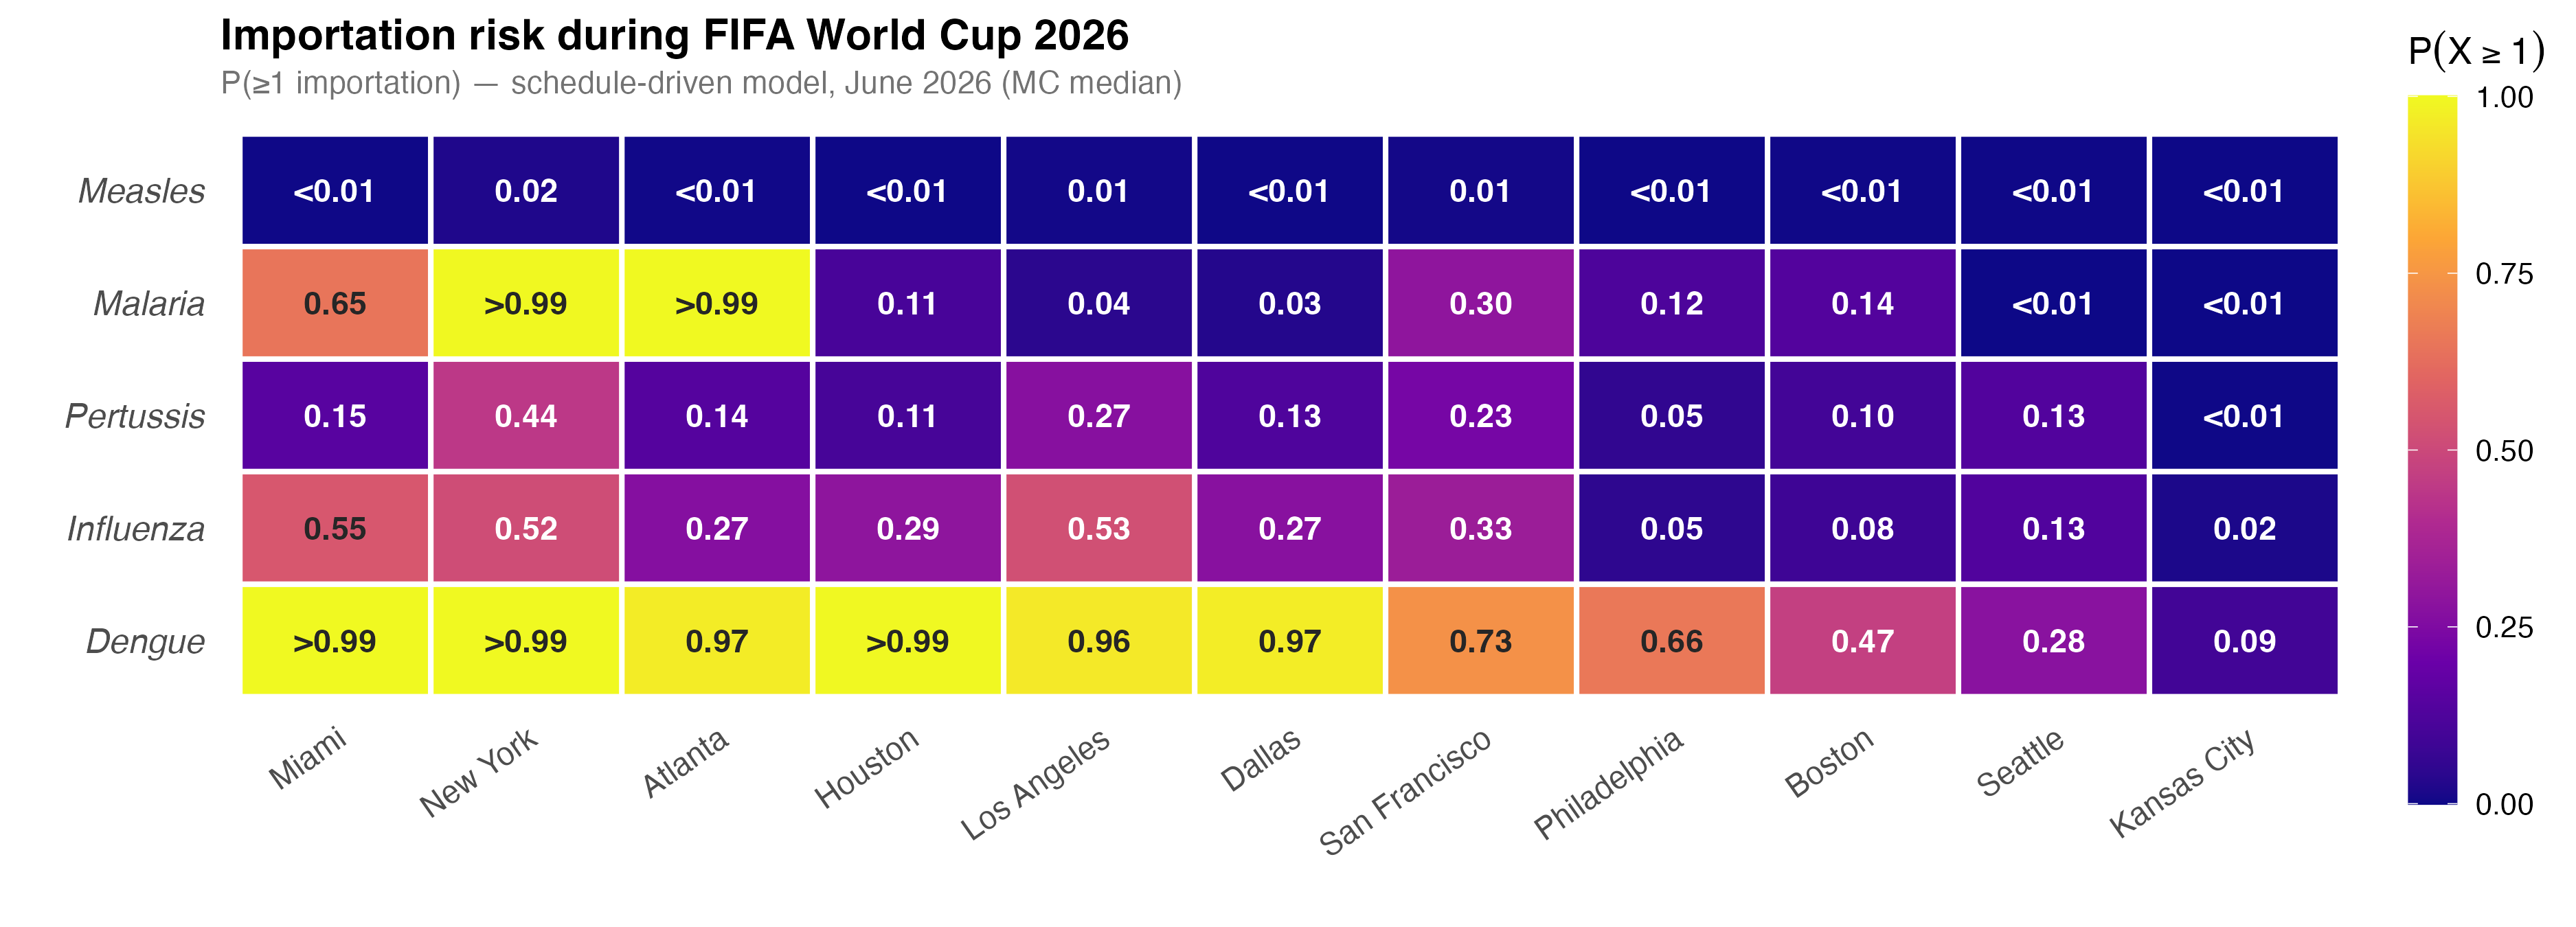
\includegraphics[width=\textwidth]{../Figures/fig1_risk_heatmap.png}
  \caption{Importation risk overview for the FIFA World Cup 2026. Each cell
    shows $P(\geq 1\text{ importation})$ under the schedule-driven model
    (Model~3), June~2026, with Monte Carlo median from 5,000 parameter draws.
    Cities are ordered left to right by decreasing aggregate importation
    intensity; diseases are ordered top to bottom by decreasing overall
    probability. Dengue importation is near-certain at every venue city;
    measles risk is the lowest of the five diseases considered.}
  \label{fig:risk_heatmap}
\end{figure}

\subsection*{Importation intensity and parameter uncertainty}

Figure~\ref{fig:lambda_ci} shows the expected importation intensity ($\Lambda$,
median and 95\% Monte Carlo uncertainty interval) per city for each disease.
For dengue, New York leads (median $\Lambda = 12.4$, 95\%~CI 6.1--30.8),
followed by Los Angeles ($\Lambda = 11.8$, CI 5.8--29.2) and Miami
($\Lambda = 10.9$, CI 5.3--27.1), driven in all cases by Brazil's combination
of high endemic burden and high June travel volume. The dengue CI extends
substantially above the median because the central detection rate $\rho = 0.10$
lies near the lower end of the literature range (0.06--0.26): true importation
intensity may be considerably higher than the central estimate.

Pertussis shows the opposite asymmetry. Its central $\rho = 0.10$ is the
\emph{upper} bound of its literature range (0.01--0.10), so the 95\%~CI
extends far below the median. Pertussis estimates are best read as conservative
upper bounds: at the lower end of the plausible detection range, expected
importations could be as low as 7\% of the median. Malaria carries a moderate,
roughly symmetric CI. Measles and influenza uncertainties are modest relative
to their medians. The directional asymmetry of each CI is visualised in
Appendix~Figure~\ref{fig:ci_asym}: diseases with upward-skewed CIs
(dengue, influenza) may be underestimated; diseases with downward-skewed CIs
(pertussis) are conservative upper bounds.

\begin{figure}[h!]
  \centering
  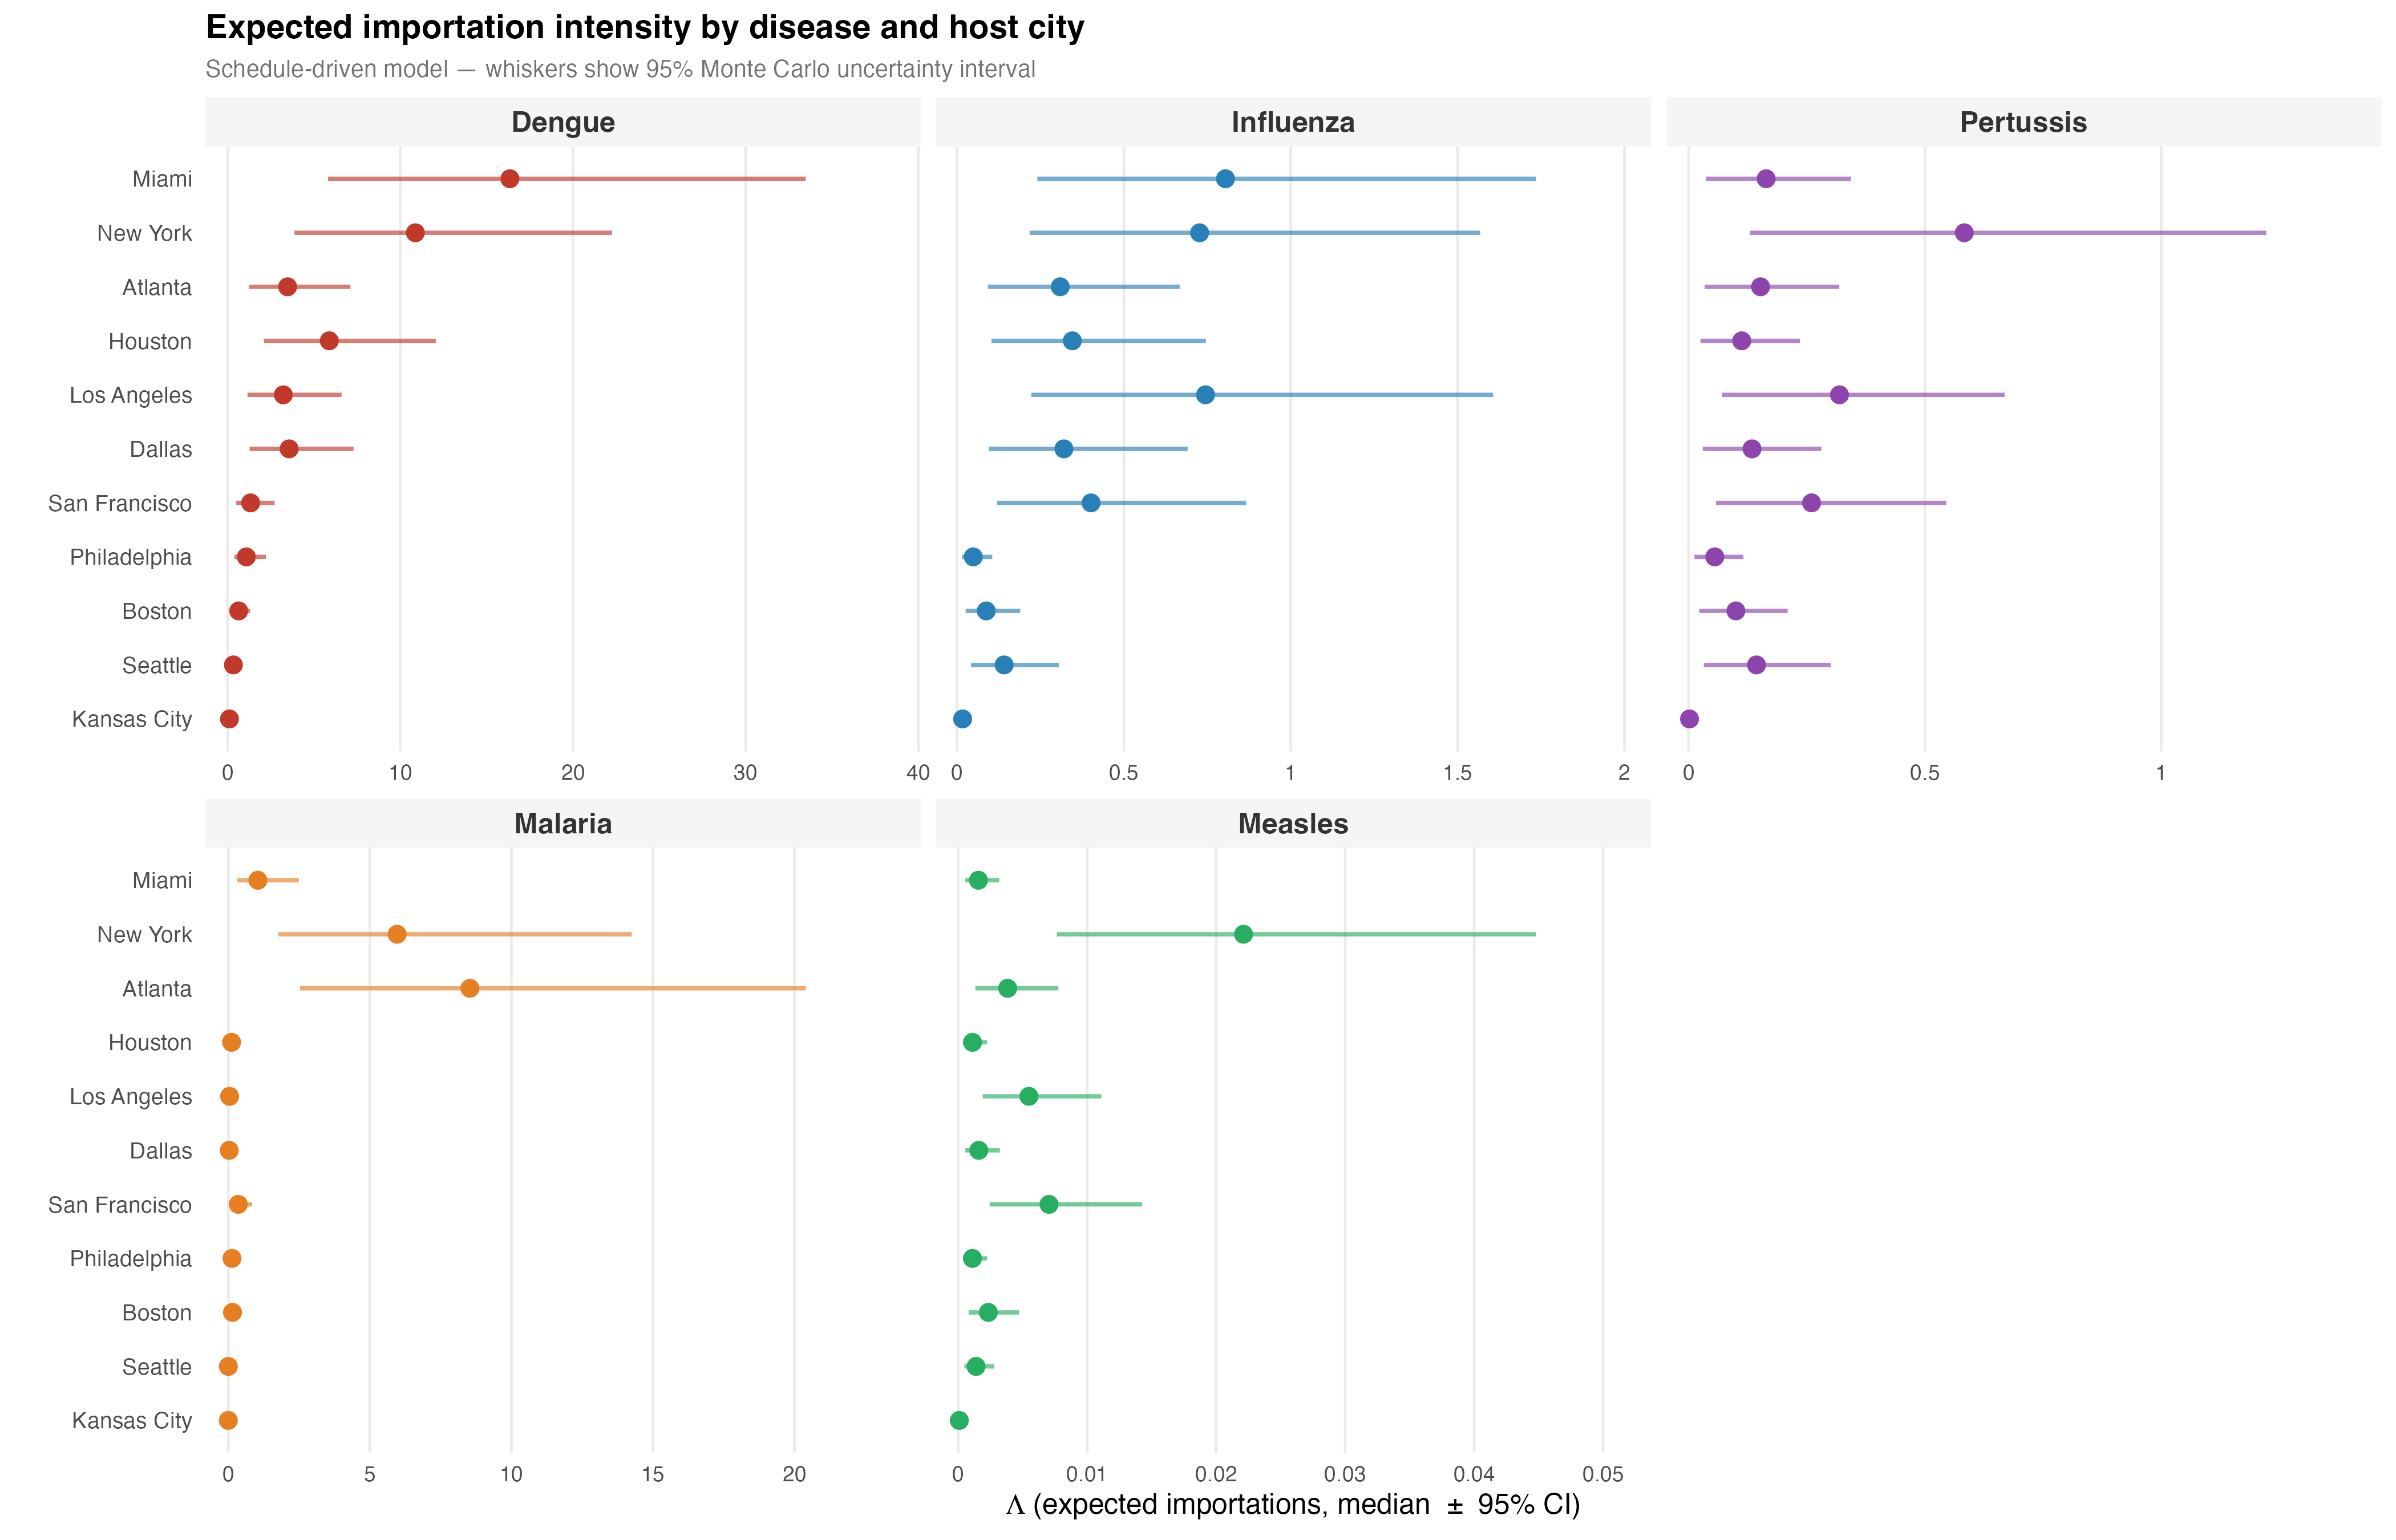
\includegraphics[width=\textwidth]{../Figures/fig2_lambda_ci.png}
  \caption{Expected importation intensity ($\Lambda$) with 95\% Monte Carlo
    uncertainty intervals under the schedule-driven model (Model~3).
    Each panel shows one disease; cities are ordered from highest to lowest
    median $\Lambda$. Points show the MC median; horizontal whiskers span the
    95\% interval (5,000 Uniform draws on $\rho_d$ and $p_d$).
    Note free x-axis scales: dengue intensity is orders of magnitude above
    the other diseases.}
  \label{fig:lambda_ci}
\end{figure}

\subsection*{World Cup travel surge: amplification without restructuring}

Figure~\ref{fig:model_comparison} compares $\Lambda$ across the three nested
model tiers for the six highest-risk US cities, with 95\% Monte Carlo
uncertainty intervals. Each panel shows one disease; within each city,
bars are grouped by model tier (Baseline, WC-adjusted, Schedule-driven),
allowing direct visual comparison of how the travel surge and schedule
routing sequentially amplify risk. The near-uniform step-up from
Model~1 to Model~2 confirms proportional amplification across cities
($\phi_\text{WC}=1.174$ vs.\ $\phi_\text{base}=1.077$; the fan increment is
approximately 8.3\% of projected arrivals for WC-qualified nations). The
further step from Model~2 to Model~3 introduces city-specific divergence:
cities hosting matches against high-incidence nations gain disproportionate
risk while cities with fewer such fixtures gain less. Kansas City, which has
limited routine international service, acquires meaningful importation risk
almost entirely through the WC-fan stream.

City rankings and the relative ordering of diseases are stable across all three
model tiers. Background tourism---travel that would occur regardless of the
tournament---accounts for the dominant share of importation risk even for
strongly WC-associated source countries such as Brazil and Colombia.
Non-qualified countries contribute exclusively through background travel.

\begin{figure}[h!]
  \centering
  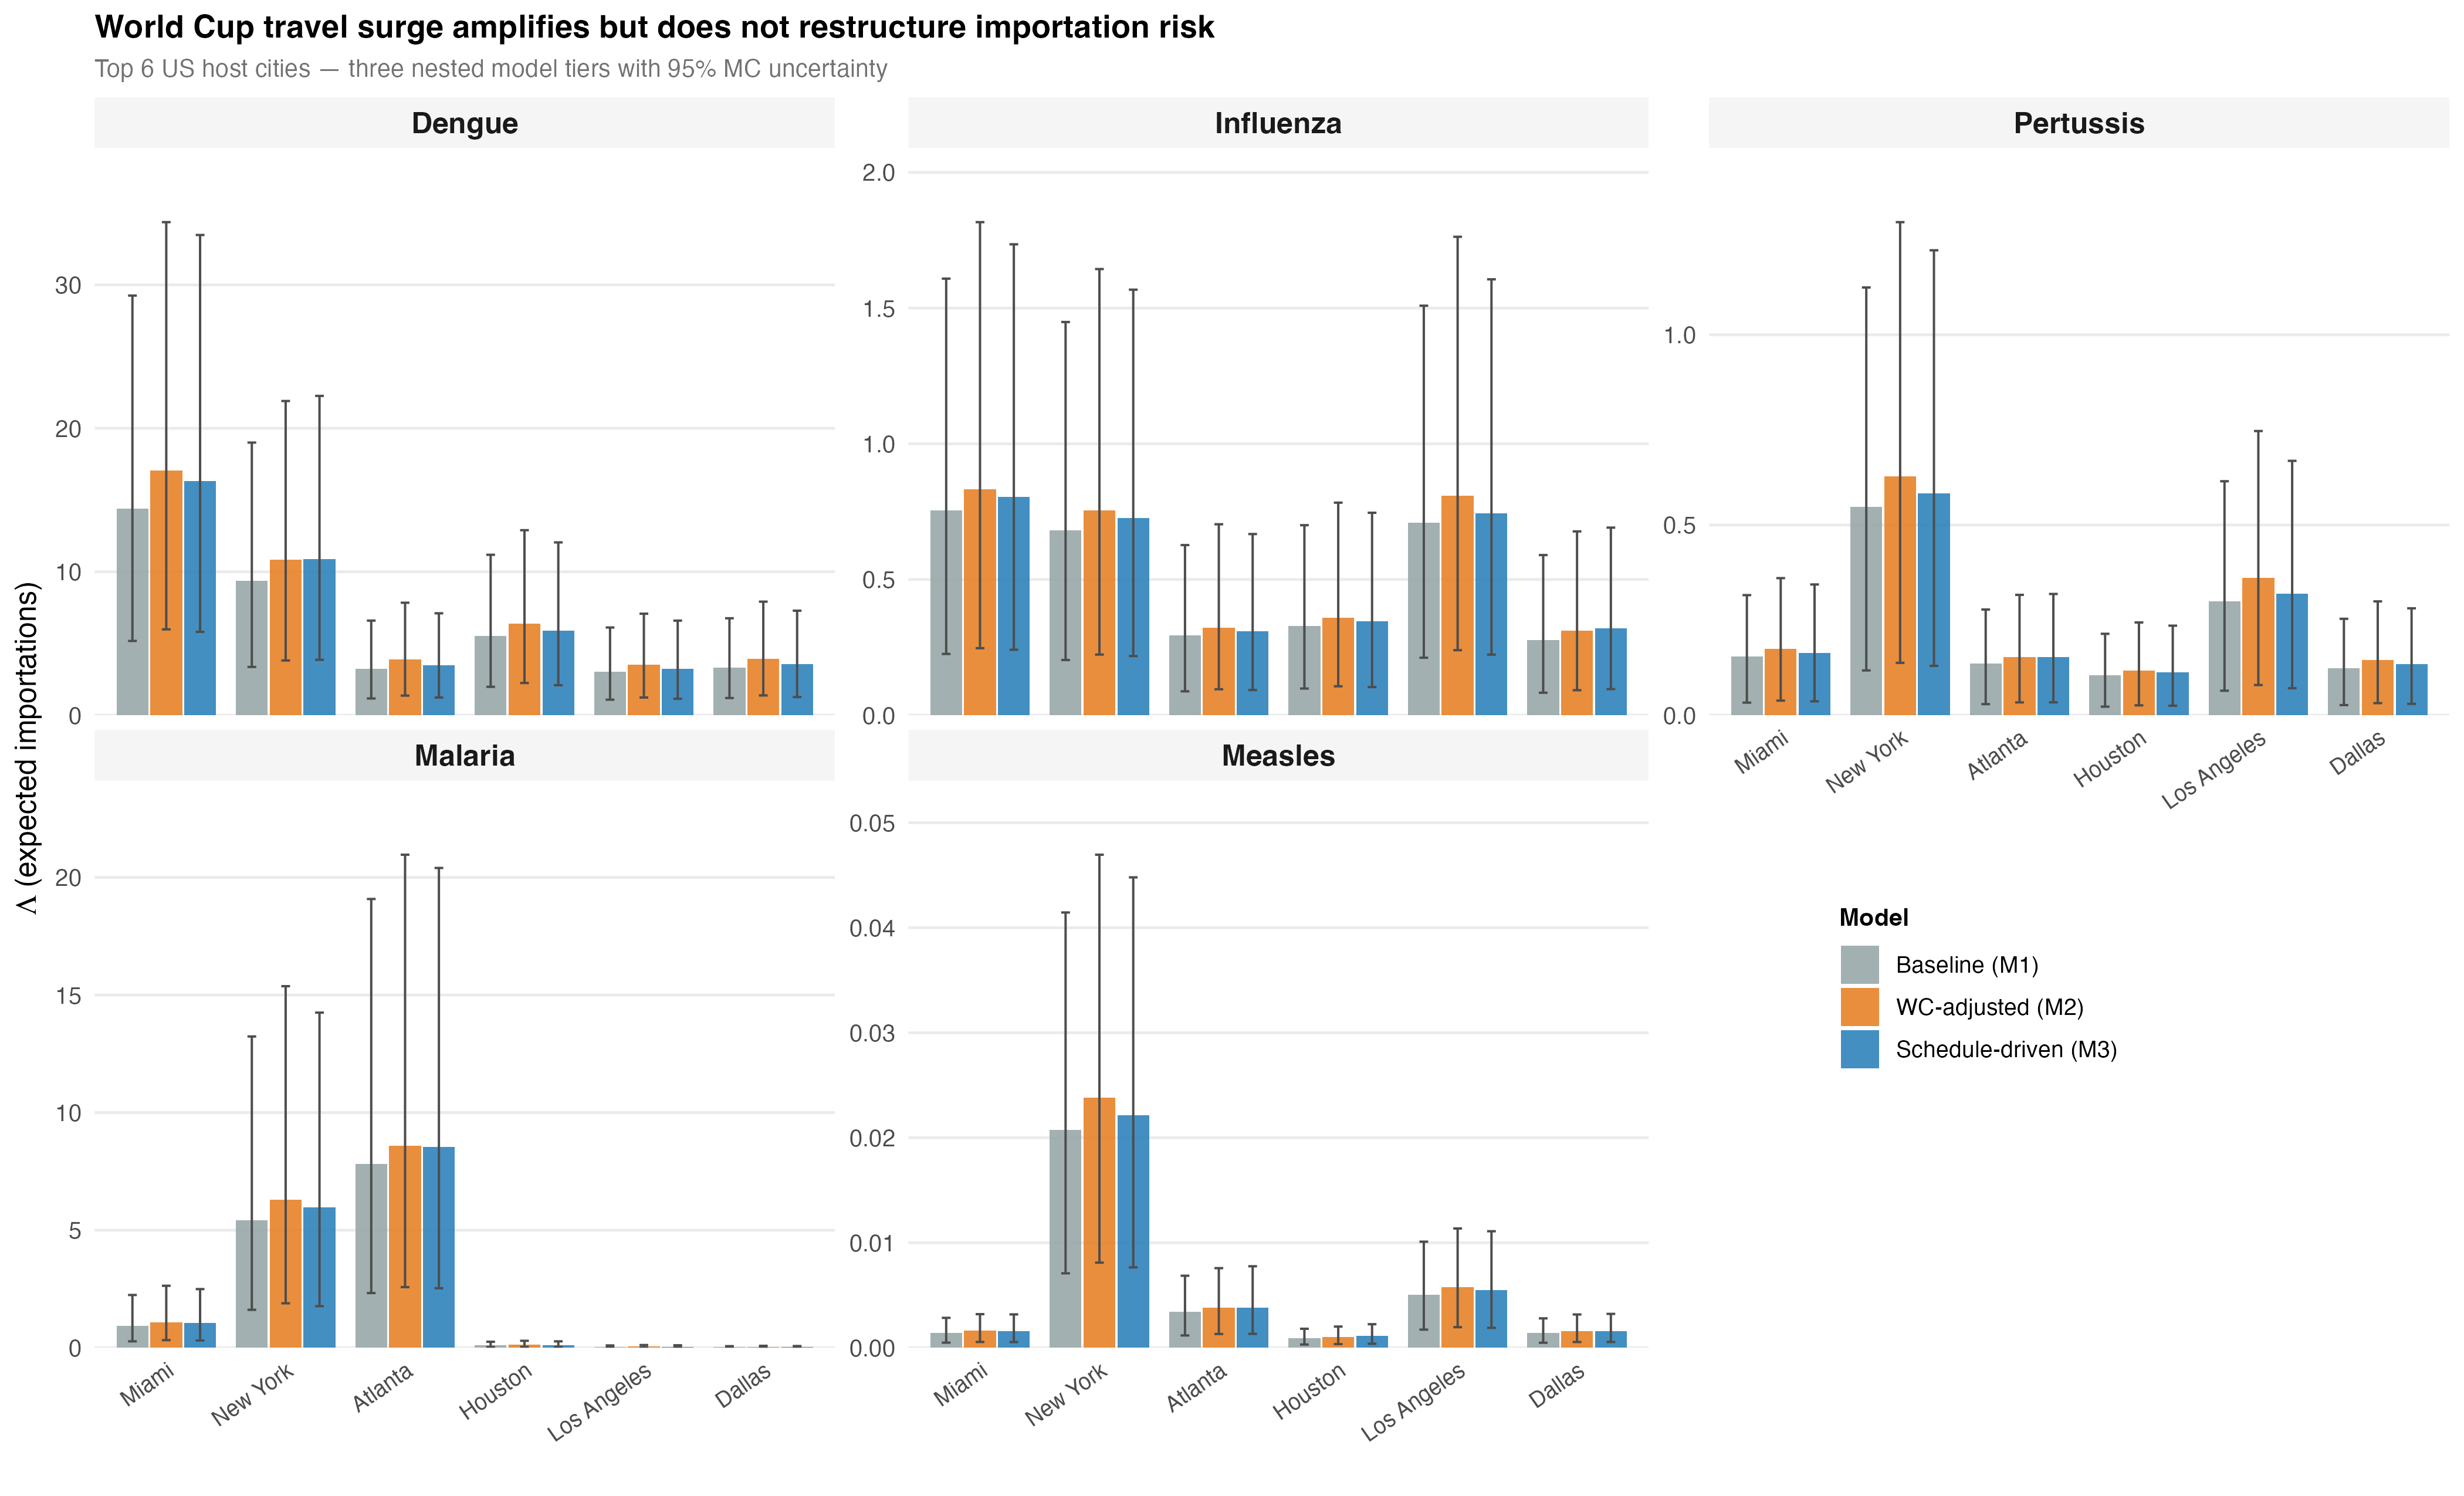
\includegraphics[width=\textwidth]{../Figures/fig3_model_comparison.png}
  \caption{Three-model comparison of expected importations ($\Lambda$) for
    the six highest-risk US venue cities. Each panel shows one disease; bars
    are grouped by city and filled by model tier: Baseline (Model~1, routine
    June~2024 travel), WC-adjusted (Model~2, June~2026 projections), and
    Schedule-driven (Model~3, fan routing by match schedule). Bars show
    the MC median; whiskers span the 95\% uncertainty interval (5,000
    Uniform draws on $\rho_d$ and $p_d$). The step-up from Model~1 to
    Model~2 is near-uniform across cities, confirming that the World Cup
    surge amplifies risk proportionally. The further step from Model~2 to
    Model~3 produces city-specific divergence driven by schedule-based
    redistribution toward match venues.}
  \label{fig:model_comparison}
\end{figure}

\subsection*{Source country drivers}

Figure~\ref{fig:country_drivers} shows the top~10 source countries by total
expected importations for each disease, coloured by world region, with 95\%
Monte Carlo uncertainty intervals. Country rankings are robust: the top three
contributors per disease are stable across the full parameter range. The
geographic pattern is disease-specific. Latin America---Brazil, Colombia,
Venezuela---dominates dengue and influenza, reflecting both high endemic burden
and the largest travel volumes to the US among WC-qualified nations. West and
Central Africa (Nigeria, Ghana, Senegal, Zaire/DRC) drives malaria risk.
European nations (Germany, the United Kingdom, France) lead pertussis and
measles, consistent with the documented pertussis resurgence and ongoing
measles circulation in Europe. Brazil is the single highest-risk source nation
overall, appearing in the top contributors for dengue, malaria, influenza, and
pertussis simultaneously.

\begin{figure}[h!]
  \centering
  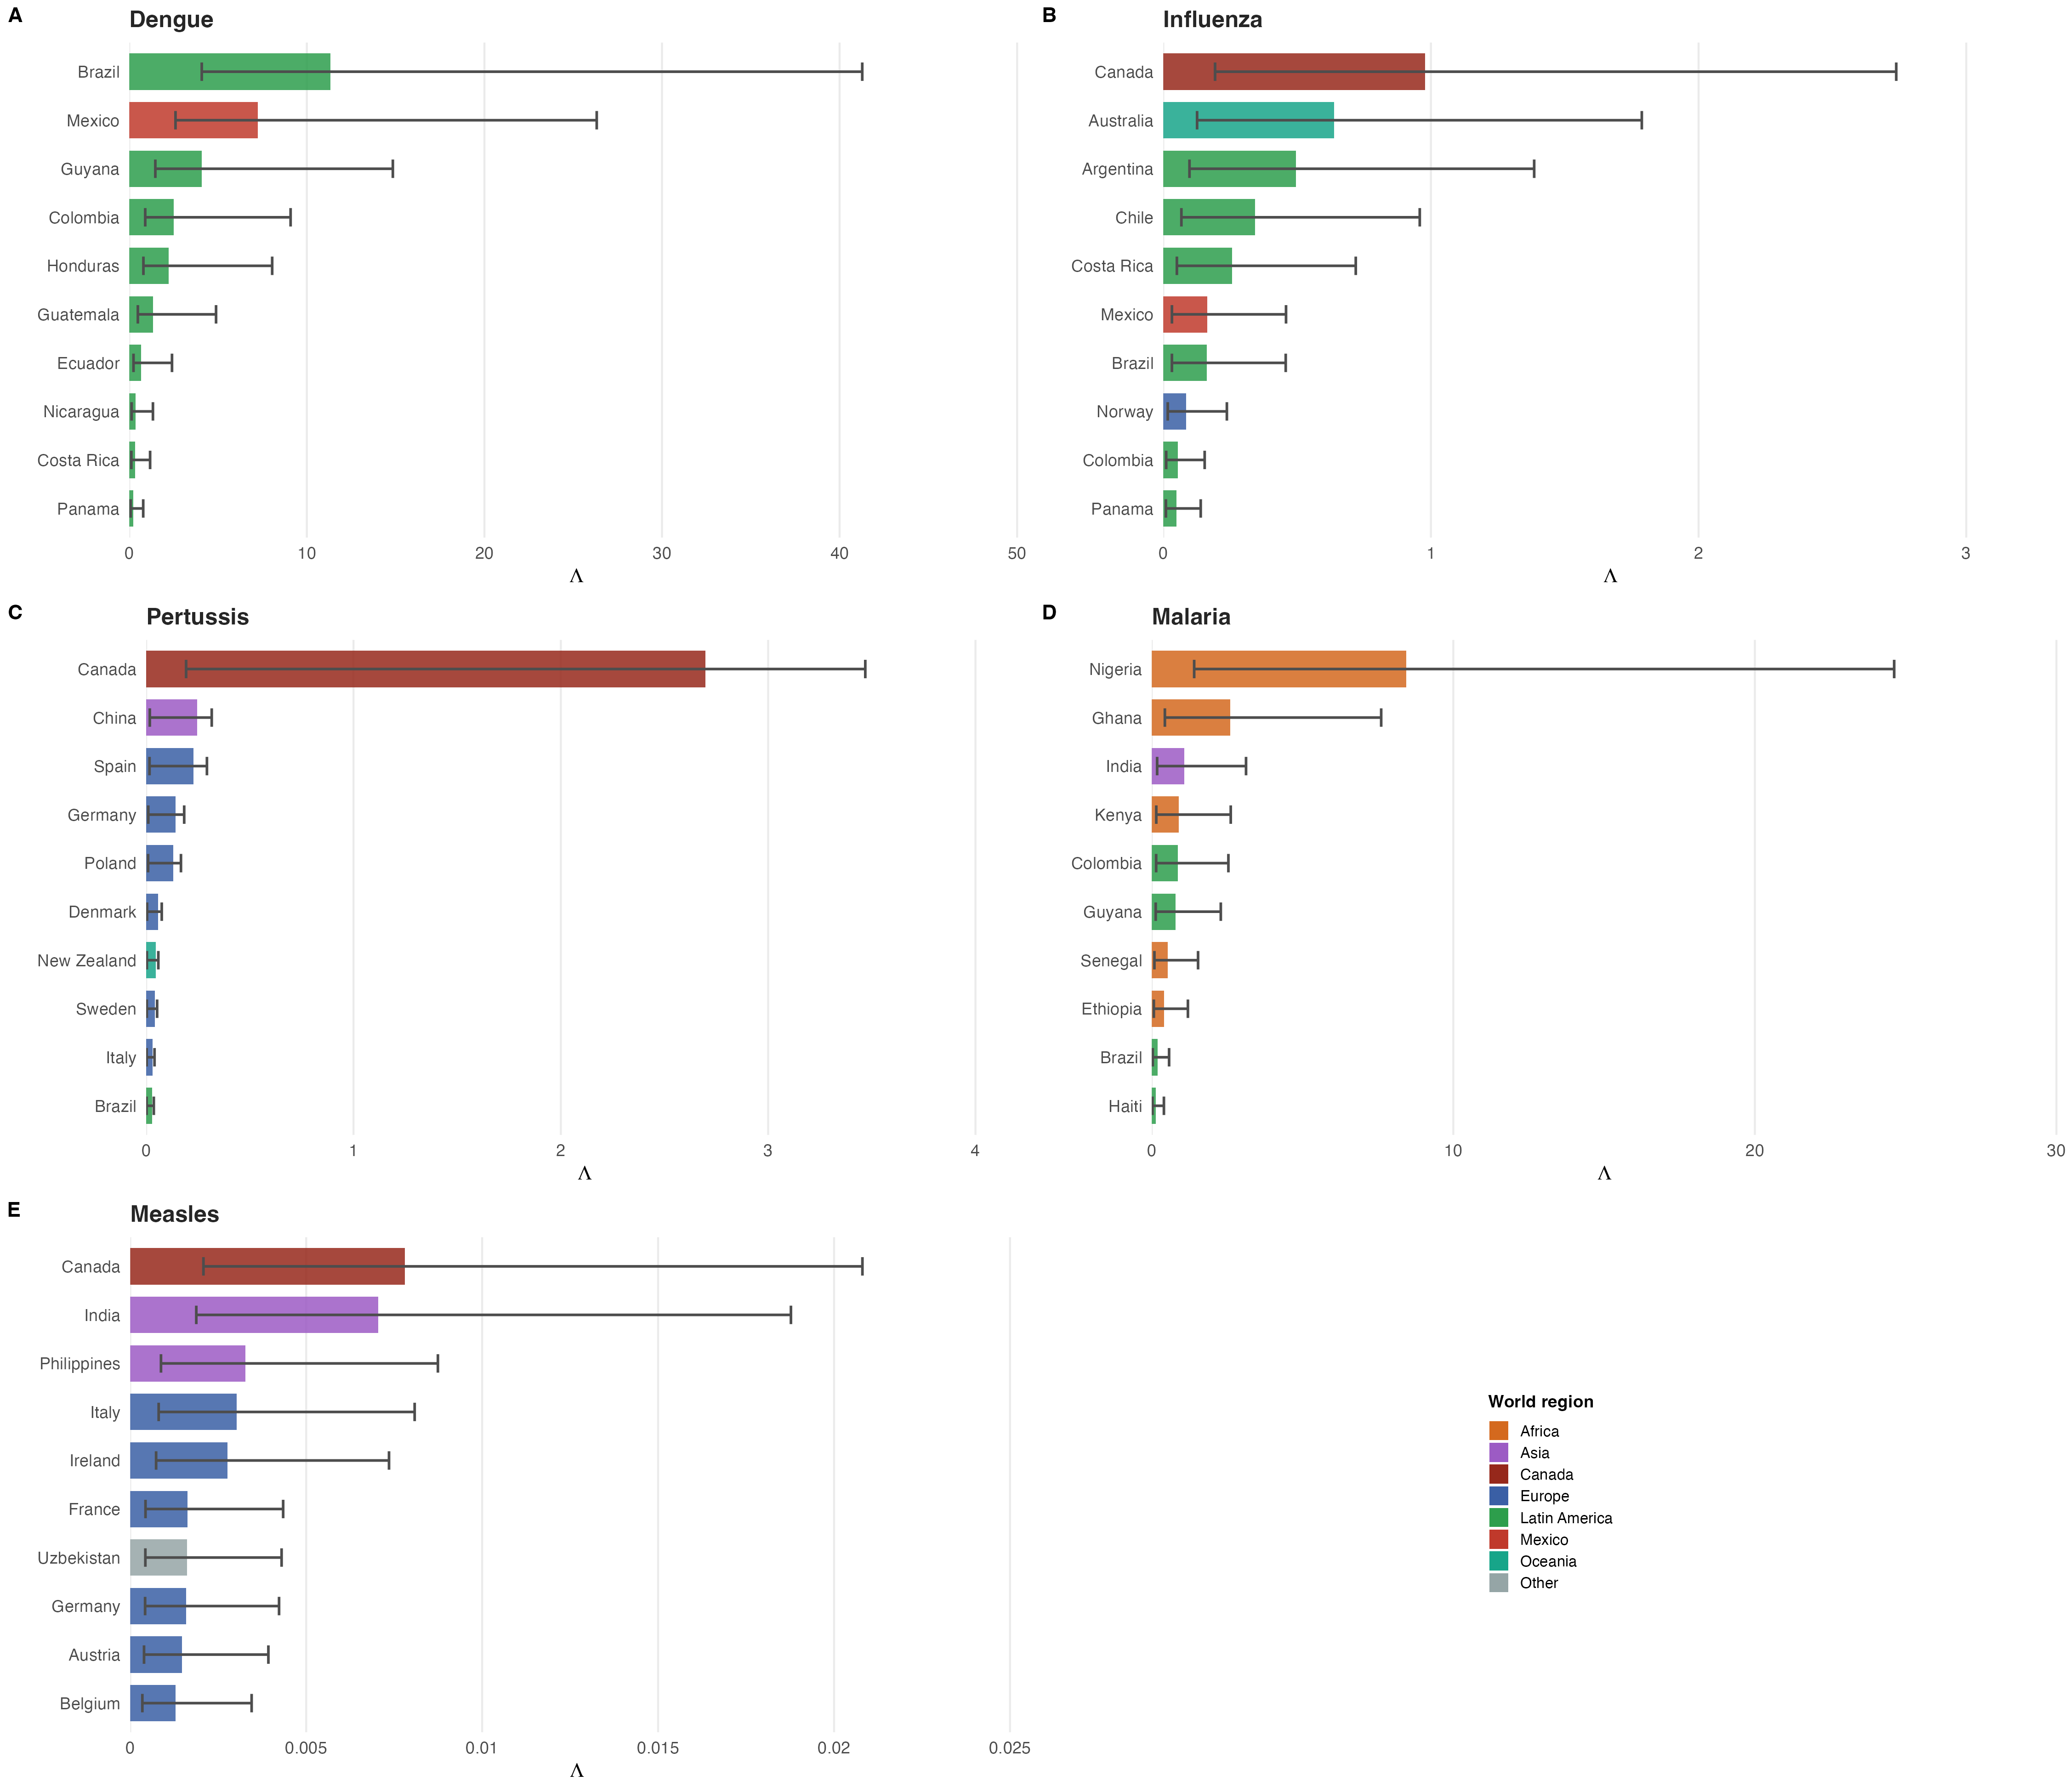
\includegraphics[width=\textwidth]{../Figures/fig4_country_drivers.png}
  \caption{Top~10 source countries by total expected importations
    (schedule-driven model, summed across all US venue cities) for each
    disease. Bars show the MC median; whiskers show the 95\% uncertainty
    interval. Colors indicate world region. Latin America dominates dengue
    and influenza risk; Africa drives malaria; Europe is the primary source
    for pertussis and measles.}
  \label{fig:country_drivers}
\end{figure}

% ============================================================
\section*{Extensions and Generalizability}
% ============================================================

Although applied here to the 2026 FIFA World Cup, the Poisson
importation framework is deliberately general. The three core
inputs---a travel volume matrix, a country-level disease incidence
table, and a travel-while-infectious probability---can be assembled
for any disease, any set of destination cities, and any international
gathering. The WC2026 application is a case study, not a constraint.

\textbf{Additional diseases.}
The model applies to any pathogen for which country-level incidence
and a travel-while-infectious probability can be specified. The
current analysis covers five diseases (dengue, influenza, malaria,
measles, pertussis); two near-term extensions are \textit{chikungunya}
and \textit{mumps}. Chikungunya poses particularly high importation
risk given the 2025--2026 outbreak in Brazil and Argentina (concurrent
analyses estimate $>$10 expected monthly imports from Brazil alone at
baseline~\cite{epistorm2026}); monthly case data are available from
PAHO and ECDC. Mumps data are available from the same WHO Immunization
portal used for measles and pertussis. Mpox (Clade I) and rubella
are lower-priority additions given low importation probabilities under
current outbreak conditions. For any newly emerging pathogen, the
framework requires only a case series by country and an estimate of
the travel-while-infectious window.

\textbf{Beyond venue cities.}
The current analysis covers the 11 US venue cities represented in
BTS T-100 routing data. The framework extends immediately to any
US city or county by substituting an alternative routing
source---DOT enplanement data, commercial booking records, or
domestic connection data---for the T-100 fraction $f_{c,v}$.
This is directly relevant for cities connected to venue cities by
domestic flights, where internationally arriving travelers may
complete their journeys on domestic legs not captured by T-100. The
same logic applies beyond the United States: any country with
international arrival records and disease surveillance data can be
modeled as a destination.

\textbf{Other mass gatherings and routine surveillance.}
The three-model hierarchy applies to any large international
gathering: Olympic Games, religious pilgrimages (e.g.,\ Hajj),
international summits, or music festivals. The only event-specific
inputs are the growth factor decomposition and the venue routing
schedule; all other components transfer directly. Beyond mass
gatherings, Model~1 functions as a standing importation surveillance
tool: updated monthly with current COR arrivals and WHO disease
data, it provides a near-real-time estimate of importation pressure
at any US airport city, independent of any scheduled event.

% ============================================================
\section*{Discussion}
% ============================================================

Integrating Monte Carlo uncertainty propagation directly into every main result---rather than relegating it to a separate appendix---is the central methodological choice of this analysis. The result is a more honest and actionable picture: dengue importation to the major US venue cities is near-certain across the full plausible parameter space, while pertussis estimates should be read as conservative upper bounds given the poorly constrained adult detection rate. The asymmetric CI structure is itself informative: diseases whose central detection rates sit at the lower end of the literature range (dengue, influenza) may be systematically underestimated, whereas diseases at the upper end (pertussis) are conservative by construction.

Applied to the 2026 World Cup, the framework reveals that importation
risk is substantial, quantifiable, and spatially heterogeneous.
The dominant empirical finding---that background tourism accounts
for the majority of importation risk even at a major international
sporting event---has an important practical implication: preparedness
efforts should not focus exclusively on World Cup fans, but should
treat the entire June international visitor population as the
exposure group of interest.

The convergence of city rankings across all three models for the
highest-risk venues (New York, Los Angeles, Miami, Houston) provides
reassurance that these results are robust to the considerable
uncertainty in WC-specific travel projections. A public health planner
who uses only the conservative Model~1 will still correctly identify
the same priority cities as a planner who uses the more complex
Model~3.

The inclusion of influenza is a distinguishing feature of this
analysis. June corresponds to the Southern Hemisphere winter
influenza peak, and WC-qualified nations in South America and Oceania
carry substantial seasonal burden during the tournament window. To
our knowledge this is the first importation risk analysis for the
2026 World Cup to quantify influenza alongside vector-borne and
vaccine-preventable diseases.

A central design goal of this analysis is accessibility: every data
source used is freely available, and all code is shared openly. This
distinguishes the approach from concurrent analyses that employ
proprietary airline booking data and commercial mobility
models~\cite{epistorm2026}. Rather than competing with those
data-intensive approaches, this framework is intended as a
reproducible baseline that any public health team can deploy,
update, and adapt without institutional data-sharing agreements or
commercial licenses. The WC2026 estimates are broadly consistent
with those of more complex models for endemically stable diseases
(dengue, malaria), validating the public-data approach for
first-order risk assessment. For outbreak-sensitive diseases, the
discrepancy between annual and rolling surveillance data---most
evident for UK measles and Norwegian pertussis---is itself a
methodological finding: it quantifies the premium on data currency
for rapidly evolving pathogens and motivates real-time data linkage
as the primary improvement pathway.

Despite its reliance on publicly available data, this framework can serve as a transparent, reproducible input to public health preparedness planning. The three-model structure maps onto a natural planning timeline: Model~1 can be run as soon as host cities are announced to establish a baseline risk ranking, Model~2 can be updated once attendance projections become available, and Model~3 can be finalised once the match schedule is confirmed. The country-level breakdowns and city-specific risk estimates can help inform decisions about which venue cities and source-country streams to prioritise for enhanced surveillance---though such decisions require additional local context (healthcare capacity, vector presence, vaccination coverage) that this model does not provide. In Model~1 mode, updated periodically with current COR arrivals and WHO surveillance data, the framework can also serve as a baseline monitoring approach for importation pressure at US international gateways between events, subject to the data-currency limitations noted below. The Monte Carlo uncertainty intervals support more transparent risk communication: rather than a single point estimate, the results convey a range that reflects genuine uncertainty in under-reporting rates and travel-while-infectious probabilities, allowing decision-makers to understand where estimates are robust and where they are not.

Several key limitations bound the scope of these estimates; full detail is given in Appendix~C. BTS T-100 data cover nonstop international segments only; passengers connecting through foreign hubs lose their country identity, and passengers connecting through US hubs are assigned to the gateway city rather than their final destination. Disease incidence is derived from annual WHO reporting cycles, which underestimate risk during active outbreaks (UK measles, European pertussis surges) and may reflect prior-year dynamics rather than the current transmission season. Growth factors $\phi_c$ are aggregate projections; actual June~2026 travel volumes will differ. The model estimates importation risk only---it does not model onward local transmission, which depends on vector presence, population immunity, and healthcare capacity not captured here. Finally, the Monte Carlo analysis propagates uncertainty in disease parameters ($\rho_d$, $p_d$) but treats travel volumes as fixed; uncertainty in the NTTO projections, T-100 routing fractions, and the WC growth factor decomposition would widen all intervals further.

The highest-priority methodological improvement is timelier disease data: substituting WHO FluNet-style rolling surveillance averages for annual incidence tables---where such data exist---would close the data-currency gap most evident for measles and pertussis. Extensions to additional diseases (chikungunya, mumps) and to domestic-connection cities beyond T-100 gateways are described in the Extensions and Generalizability section above. Longer term, coupling importation estimates with local vector surveillance and population immunity data would enable a full importation-to-transmission risk pathway, the primary gap between what this framework currently provides and what would be needed for outbreak probability estimation.

% ============================================================
\section*{Conclusions}
% ============================================================

We present a general, reproducible Poisson framework for quantifying
infectious disease importation risk that requires only publicly
available travel and surveillance data. The framework is applicable
to any disease, any destination city with international arrivals,
and any mass gathering or routine surveillance context. Applied to
the 2026 FIFA World Cup across five diseases and 11 US venue cities,
dengue fever emerges as the primary importation concern, with New
York, Los Angeles, Miami, and Houston at highest aggregate risk.
Influenza ranks second, reflecting its Southern Hemisphere winter
peak during the June tournament window. Background international
travel---not World Cup fan travel specifically---is the dominant
risk driver for all diseases, a finding with direct implications for
surveillance prioritization at any international event.

% ============================================================
\bibliographystyle{unsrtnat}
\bibliography{references}

\newpage
\appendix

% ============================================================
\section*{Appendix A: Detailed Methods and Data Sources}
% ============================================================

\subsection*{Study setting}

The 2026 FIFA World Cup will be hosted jointly by the United States,
Mexico, and Canada, with matches scheduled from June~11 through
July~19, 2026. The United States will host the majority of matches
across eleven venues: MetLife Stadium (East Rutherford, NJ), SoFi
Stadium (Inglewood, CA), AT\&T Stadium (Arlington, TX), Mercedes-Benz
Stadium (Atlanta, GA), NRG Stadium (Houston, TX), Arrowhead Stadium
(Kansas City, MO), Lincoln Financial Field (Philadelphia, PA), Hard
Rock Stadium (Miami Gardens, FL), Levi's Stadium (Santa Clara, CA),
Lumen Field (Seattle, WA), and Gillette Stadium (Foxborough, MA).
Canada hosts two venues (BC~Place, Vancouver; BMO~Field, Toronto) and
Mexico hosts three (Estadio~Azteca, Mexico City; Estadio~BBVA,
Monterrey; Estadio~Akron, Guadalajara). The geographic distribution
of all 16 venues across the three co-host nations is shown in
Figure~\ref{fig:venue_map}.
All 48 qualified nations are listed in Supplementary Table~1.

\begin{figure}[h!]
  \centering
  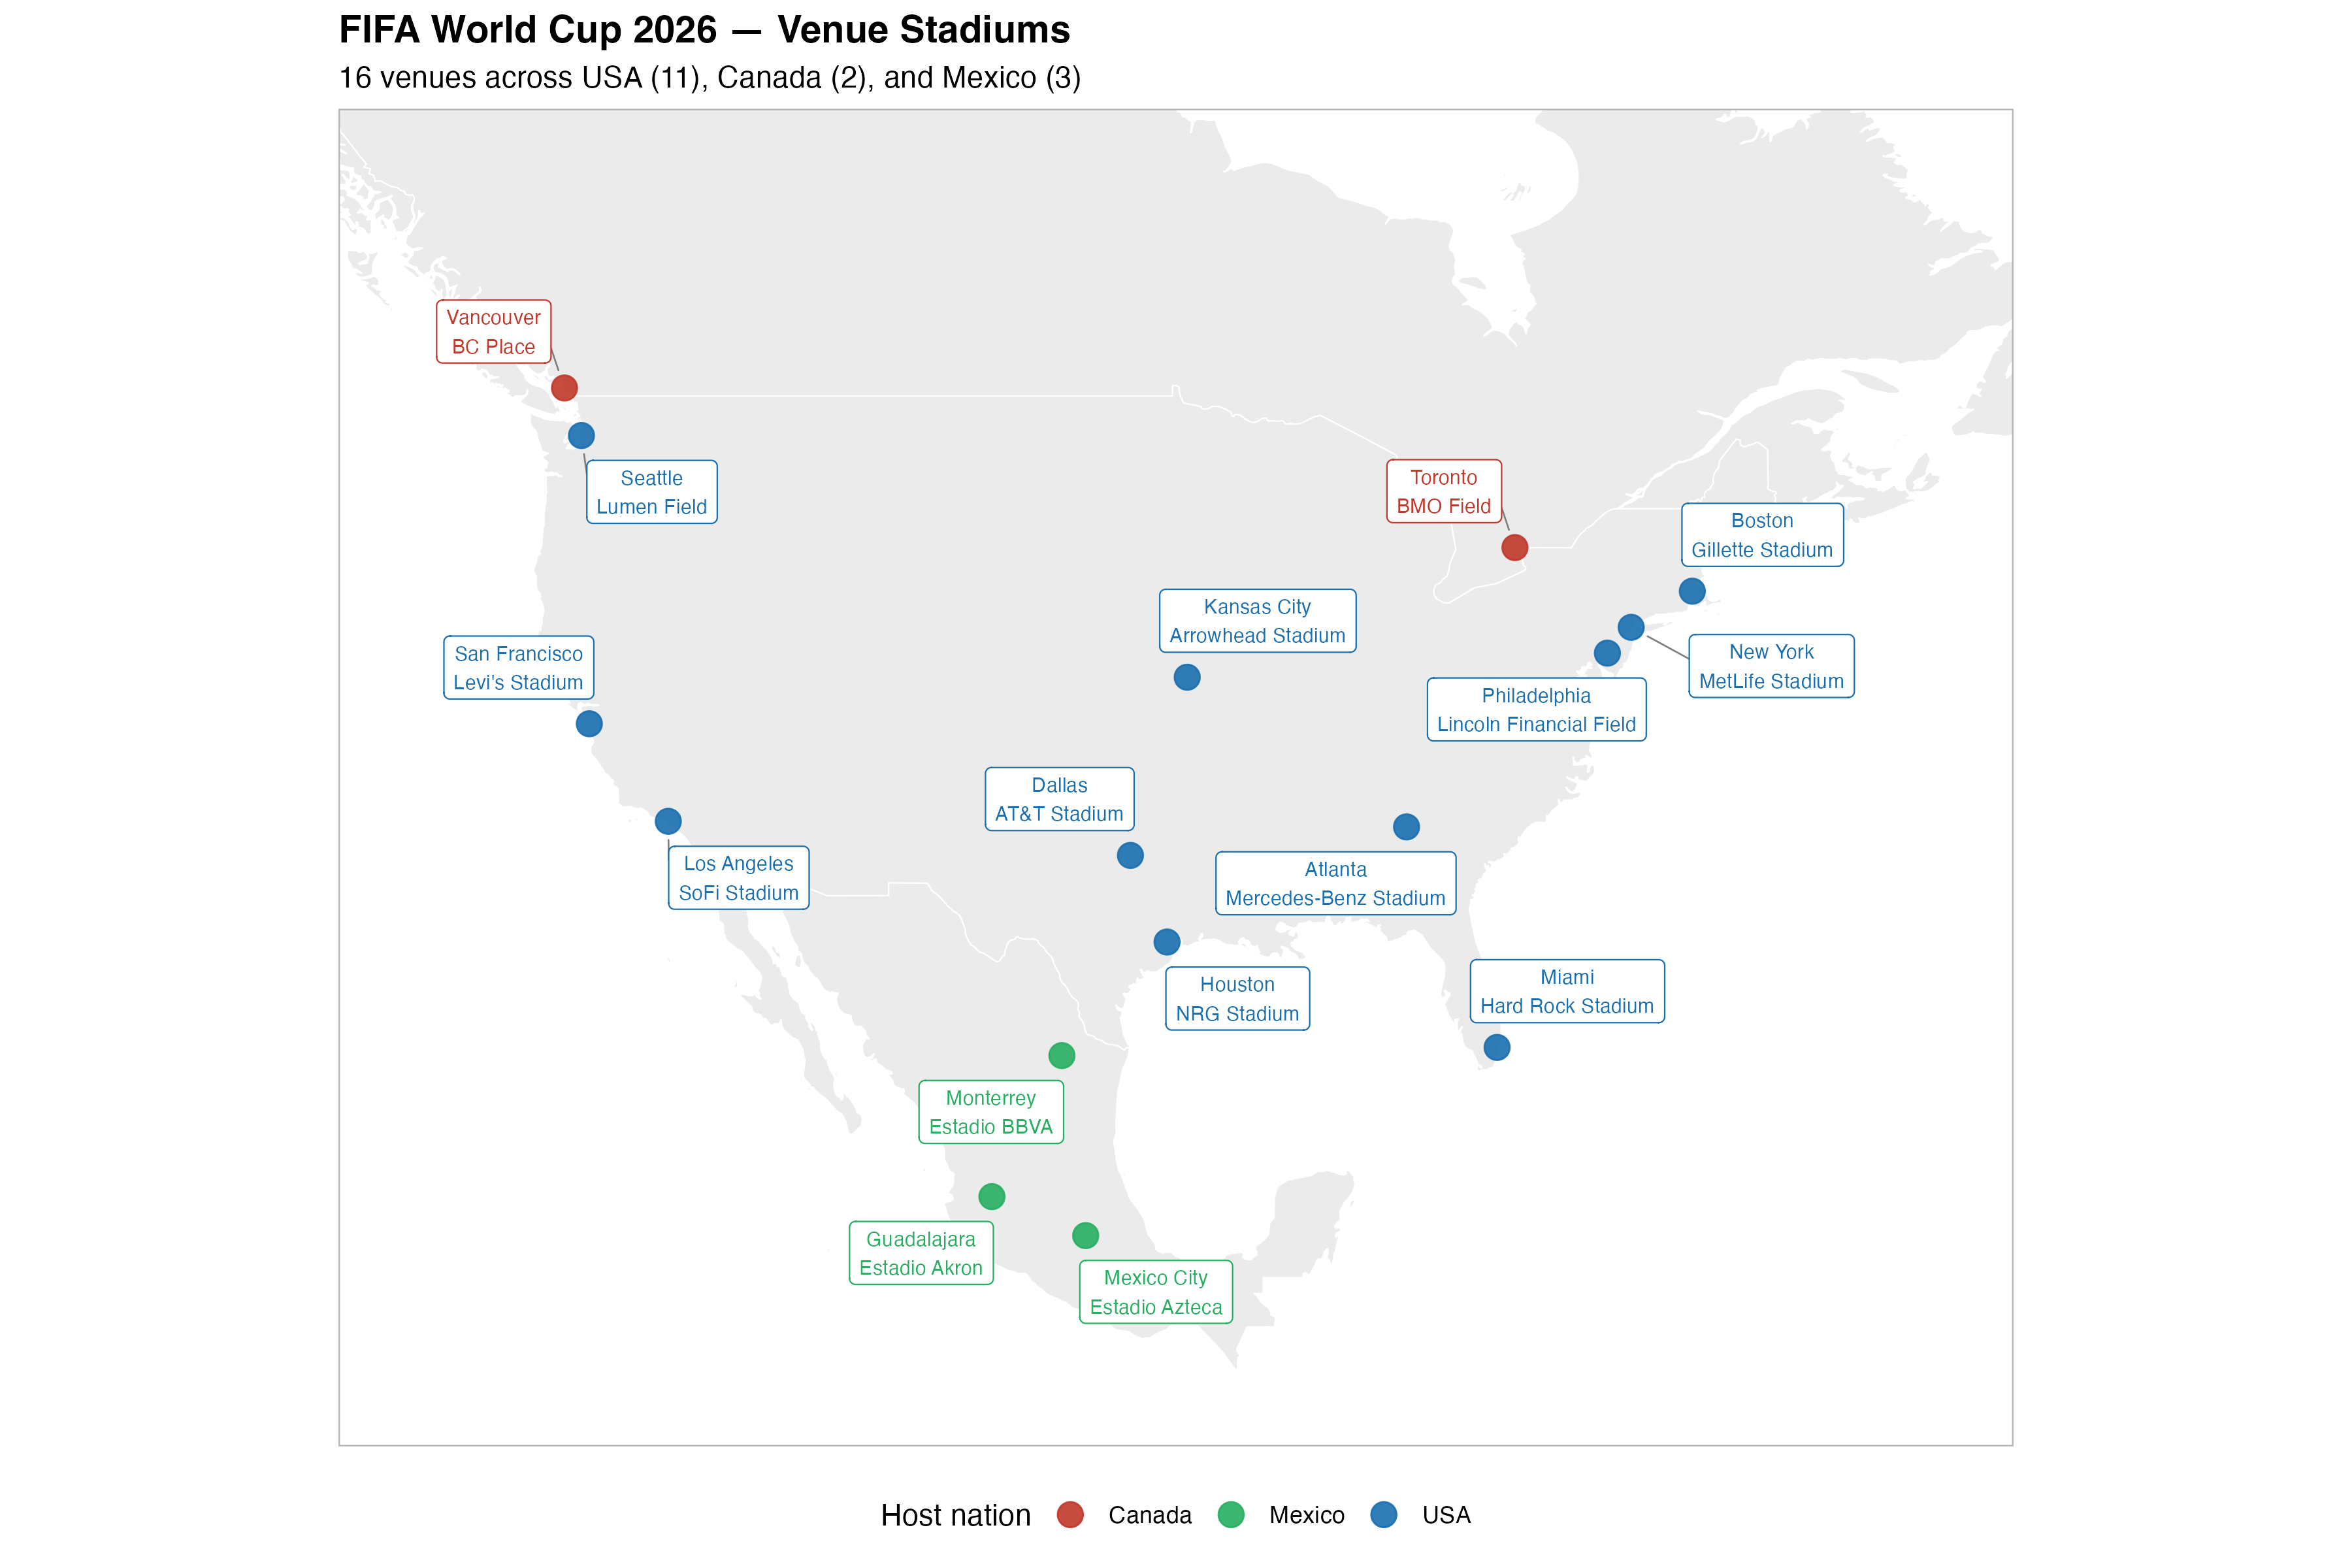
\includegraphics[width=\textwidth]{../Figures/wc2026_venue_map.png}
  \caption{Geographic distribution of the 16 FIFA World Cup 2026
    venue stadiums across the three co-host nations. Circles are
    colour-coded by host country: USA (blue, 11 venues), Canada
    (red, 2 venues), and Mexico (green, 3 venues). Suburb stadium
    locations are labelled by their metropolitan area to match the
    spatial aggregation used throughout the analysis
    (e.g.\ East Rutherford $\to$ New York, Foxborough $\to$ Boston).}
  \label{fig:venue_map}
\end{figure}

We estimated the importation risk of five infectious diseases---dengue
fever, influenza, malaria, measles, and pertussis---for each host city
using three complementary models of increasing resolution: (1) a
\emph{baseline model} using COR June 2024 arrivals with BTS T-100
routing fractions and no World Cup growth adjustment; (2) a \emph{World
Cup (WC)-adjusted model} that scales volumes to country-level 2026
projections; and (3) a \emph{schedule-driven model} that separates
World Cup fan travel from background tourism and routes fans to the
specific venue cities where their national team plays.
The five diseases were selected because each is endemic in countries
with strong football traditions, each has a plausible pathway for
travel-associated importation into the United States, and each
represents a distinct surveillance and public health response
challenge. Influenza is included because June corresponds to the
Southern Hemisphere winter peak, coinciding with the tournament window
for WC-qualified nations in South America and Oceania.

% ============================================================
\subsection*{Notation and variable definitions}

The following indices and variables are used consistently throughout
all three models. Where the range of an index differs between models,
this is noted explicitly.

\vspace{0.5em}
\noindent\textbf{Indices}
\begin{itemize}
  \item $c$ --- source \textbf{country} of international travelers
    (all three models).
  \item $v$ --- \textbf{destination venue city}. In all three models,
    $v$ ranges over the eleven US WC venue cities
    (Table~\ref{tab:venues}). Model~3 additionally covers the five
    non-US host cities (Toronto, Vancouver, Guadalajara, Mexico City,
    Monterrey).
  \item $d$ --- \textbf{disease}: $d \in \{\text{dengue},\,
    \text{influenza},\, \text{malaria},\, \text{measles},\,
    \text{pertussis}\}$.
  \item $y$ --- \textbf{calendar year}, used when averaging over
    multiple June cross-sections ($y \in \{2023, 2024, 2025\}$ for
    T-100 routing fractions).
\end{itemize}

\vspace{0.5em}
\noindent\textbf{Travel and importation variables}
\begin{itemize}
  \item $N_{c,v}$ --- expected number of \textbf{travelers} from
    source country $c$ arriving in city $v$ during June.
    Constructed differently in each model (see below).
  \item $\Lambda_{v,d}$ --- \textbf{importation intensity} (Poisson
    rate): expected number of imported cases of disease $d$ arriving
    in city $v$ during June 2026.
  \item $\lambda_{c,v,d}$ --- \textbf{importation contribution}
    from source country $c$ to city $v$ for disease $d$;
    $\Lambda_{v,d} = \sum_c \lambda_{c,v,d}$.
\end{itemize}

\vspace{0.5em}
\noindent\textbf{Disease and parameter variables}
\begin{itemize}
  \item $I_{c,d}$ --- \textbf{per-traveler infection probability}:
    probability that a randomly selected traveler from country $c$
    is carrying disease $d$ during their trip. Defined as
    $I_{c,d} = \rho_d \cdot C_{c,d} / P_c$.
  \item $C_{c,d}$ --- \textbf{reported cases} of disease $d$ in
    source country $c$ during June (or annual figure divided by 12 for
    diseases with only annual reporting).
  \item $P_c$ --- \textbf{population} of source country $c$.
  \item $\rho_d$ --- \textbf{reporting adjustment factor} for
    disease $d$: corrects for under-reporting in routine
    surveillance and the fraction of reported cases that are
    actively infectious at any given time
    (Table~\ref{tab:params}).
  \item $p_d$ --- \textbf{travel-while-infectious probability}:
    probability that a person infected with disease $d$ continues
    to travel internationally during the infectious window
    (Table~\ref{tab:params}).
\end{itemize}

\vspace{0.5em}
\noindent\textbf{Routing fractions and travel growth}
\begin{itemize}
  \item $f_{c,v}^{\text{T100}}$ --- \textbf{T-100 routing fraction}:
    share of country $c$'s US-bound June arrivals that enter through
    city $v$, derived from BTS T-100 International Segment data
    averaged over June 2023--2025. Used in all three models.
  \item $\phi_c$ --- \textbf{growth factor} for country $c$:
    ratio of projected 2026 to observed 2024 annual visitor volume
    ($\phi_c = V_{c,2026}/V_{c,2024}$). Derived from NTTO for Tier~1
    countries; set to $\phi_{\text{WC}}$ or $\phi_{\text{base}}$ for
    all others.
  \item $\phi_{\text{WC}} = 1.174$ --- aggregate WC growth factor
    (NTTO total: 85,017/72,390 thousand).
  \item $\phi_{\text{base}} = 1.077$ --- baseline (non-WC) growth
    factor derived as the geometric mean annual growth rate over
    June 2023--2025, averaged across COR (1.062) and T-100 (1.092)
    data sources; applied to non-qualified countries.
  \item $N_c^{\text{WC}}$ --- \textbf{WC-fan travel increment}:
    marginal arrivals attributed to the World Cup for country $c$.
  \item $N_c^{\text{bg}}$ --- \textbf{background arrivals}: June
    2026 travel that would have occurred without the WC.
  \item $\omega_{c,v}$ --- \textbf{schedule routing fraction}:
    share of WC fans from country $c$ attending matches in venue
    city $v$; defined as games played in $v$ divided by total known
    games for that team.
  \item $\mathcal{Q}$ --- set of WC-qualified countries with a
    known group-stage match schedule (TBD matches excluded).
\end{itemize}

% ============================================================
\subsection*{Importation risk framework}

We modelled disease importation as a Poisson process. This choice
is standard for rare-event counting problems: when individual import
events are independent and the per-traveller probability of infection
is small, the number of imported cases in a fixed time window
converges to a Poisson random variable. The Poisson framework is also
analytically tractable and additive over source units, allowing
country-level and stream-level contributions to be computed and
summed independently.

If $\Lambda_{v,d}$ is the expected number of imported cases of disease
$d$ arriving in city $v$ during June 2026, the probability of
observing at least one importation is:

\begin{equation}
  P(X_{v,d} \geq 1) = 1 - e^{-\Lambda_{v,d}}
  \label{eq:poisson}
\end{equation}

where $\Lambda_{v,d} = \sum_{c} \lambda_{c,v,d}$ sums over all origin
countries $c$. This framework is consistent with previously
published importation risk analyses for large international sporting
events~\cite{Herrera2024}.

Each country-level contribution takes the same multiplicative form
across all three models:
\begin{equation}
  \lambda_{c,v,d} = N_{c,v} \cdot I_{c,d} \cdot p_d
  \label{eq:general_lambda}
\end{equation}
where $N_{c,v}$ is the number of travellers from country $c$ arriving
in city $v$, $I_{c,d}$ is the per-traveller probability that an
arriving person carries disease $d$, and $p_d$ is the probability
that such a person travels internationally while infectious. The three
models differ in how $N_{c,v}$ and $I_{c,d}$ are constructed.

% ============================================================
\subsection*{Baseline model: COR June 2024 travel volume with T-100 routing
(no WC adjustment)}

\subsubsection*{Rationale and design}

The baseline model establishes the importation risk expected in a
typical June \emph{without} any World Cup effect. Its purpose is to
provide a pre-tournament reference against which the WC-driven
changes in Models~2 and~3 can be measured. Three design choices
ensure this reference is both accurate and spatially consistent:

\begin{enumerate}
  \item \textbf{Travel volume: COR June 2024, no growth factor.}
    Monthly air arrivals by country of residence (COR/I-94) for
    June 2024 are used directly, without any WC growth factor
    ($\phi_c = 1$ for all countries). June 2024 is the most recent
    pre-tournament June with complete data and represents normal
    summer travel patterns.

  \item \textbf{City routing: BTS T-100 routing fractions.}
    Country-level routing fractions $f_{c,v}^{\text{T100}}$
    (described in the next subsection and in
    Equation~\ref{eq:t100_routing}) allocate each country's COR
    arrivals to the eleven US venue cities. Using T-100 from the
    baseline ensures all three models operate on the same spatial
    grid, making the three-way comparison interpretable: the step
    from Model~1 to Model~2 isolates the WC travel surge alone,
    not a change in routing methodology.

  \item \textbf{Disease incidence: country-level.}
    Country-specific incidence proxies $I_{c,d}$ are used
    (Equation~\ref{eq:country_inc}), providing the same precision
    as Models~2 and~3 and ensuring that differences between models
    reflect travel volume changes, not incidence aggregation.
\end{enumerate}

\subsubsection*{Baseline city-level arrivals}

Baseline arrivals from country $c$ to venue city $v$ are:
\begin{equation}
  N_{c,v}^{\text{baseline}} = N_{c,\text{June 2024}}^{\text{COR}}
    \cdot f_{c,v}^{\text{T100}}
  \label{eq:baseline_arrivals}
\end{equation}

Countries with no T-100 routing data (typically nations with no
scheduled nonstop international service to the United States) are
excluded; their volumes are negligible in the aggregate.

\subsubsection*{Importation intensity (baseline)}

\begin{equation}
  \lambda_{c,v,d} = N_{c,v}^{\text{baseline}} \cdot I_{c,d} \cdot p_d
  \label{eq:lambda_baseline}
\end{equation}

\begin{equation}
  \Lambda_{v,d} = \sum_{c} \lambda_{c,v,d}
\end{equation}

The probability of at least one importation is computed via
Equation~\ref{eq:poisson}.

% ============================================================
\subsection*{BTS T-100 International Segment data: country-level
city routing fractions}

\subsubsection*{Motivation and data source}

All three models require country-level city routing fractions that
cover every US WC venue city. We use the Bureau of Transportation
Statistics (BTS) T-100 International Segment (All Carriers)
dataset~\cite{BTS_T100}, which records nonstop international flight
segments landing at US airports at the individual airport level.
T-100 covers all US commercial airports and reports passengers by
country of origin (via the departure country code), making it
possible to compute country-specific routing fractions for all eleven
US venue cities. The T-100 data do not include an origin city field,
only the originating country code for the international segment.

\subsubsection*{Data processing and routing fraction construction}

Three full years of T-100 data were downloaded for 2023, 2024, and
2025, covering all months. Only June records (month = 6) were
retained for each year, yielding three June cross-sections. This
window was chosen to: (1) match the June travel period of the WC
group stage; (2) use the three most recent complete pre-tournament
June months; and (3) avoid the COVID-recovery period (2020--2022)
during which route networks and traffic volumes were atypical.

Records were filtered to scheduled passenger service only
(\texttt{CLASS = "F"}), excluding charter (\texttt{N}),
all-cargo (\texttt{L}), and mixed cargo (\texttt{P}) service
classes. Only segments with at least one passenger (\texttt{PASSENGERS > 0})
and landing in the United States (\texttt{DEST\_COUNTRY = "US"}) were
retained. Destination airports were then mapped to the eleven US
WC venue city groups using a predefined airport-to-city table (e.g.,
JFK, EWR, and LGA $\to$ New York; MIA and FLL $\to$ Miami;
SFO, OAK, and SJC $\to$ San Francisco). Any airport not associated
with a WC venue city was excluded.

For each source country $c$, venue city $v$, and year $y$, the
routing fraction is first computed within each June cross-section
as:
\begin{equation}
  f_{c,v,y}^{\text{T100}} =
    \frac{N_{c,h,y}^{\text{June}}}
         {N_{c,\text{US},y}^{\text{June}}}
\end{equation}
where $N_{c,h,y}^{\text{June}}$ is the total T-100 passengers from
country $c$ to the airport group serving venue city $v$ in June of
year $y$, and $N_{c,\text{US},y}^{\text{June}}$ is the total T-100
passengers from country $c$ to \emph{all} US airports in June of
year $y$ (the denominator). Using the full US total---not just WC
venue airports---ensures that fractions are true proportions,
interpretable as the share of US-bound travel from country $c$ that
enters through each city.

The mean routing fraction is then averaged across the three years:
\begin{equation}
  f_{c,v}^{\text{T100}} = \frac{1}{|Y|}
    \sum_{y \in Y} f_{c,v,y}^{\text{T100}}
  \label{eq:t100_routing}
\end{equation}
where $Y = \{2023, 2024, 2025\}$. Averaging within years before
averaging across years (rather than pooling all passenger counts)
prevents high-volume years from dominating the estimate and keeps
each annual fraction a valid proportion.

\subsubsection*{Important limitations of T-100 routing fractions}

T-100 records the \emph{nonstop international segment} only. A
passenger travelling on a connecting itinerary (e.g., São Paulo
$\to$ Miami $\to$ Kansas City) appears only in the Miami row, because
Miami is the airport where the international segment terminates and US
Customs is cleared. Kansas City, as a domestic connecting leg, is not
recorded in T-100 for that passenger. This is the correct
interpretation for importation risk modelling: from a public health
perspective, the traveller enters the US in Miami, where surveillance
and border health screening occurs. Kansas City correctly shows
near-zero T-100 routing fractions for most countries, reflecting
minimal direct international service; its WC-specific traffic is
captured entirely by the schedule-driven WC-fan stream.

The T-100 data cover US airports only. Routing fractions for the five
non-US host cities (Toronto, Vancouver, Guadalajara, Mexico City,
Monterrey) cannot be derived from T-100 and are not estimated here;
those cities receive importation risk estimates solely from the
WC-fan travel stream.

Country names in T-100 use ISO/ICAO conventions (e.g.,
``Korea, Republic of'', ``Viet Nam'') while the CBP COR arrival data
use informal short names (e.g., ``South Korea'', ``Vietnam''). A
standardised recode table covering 26 known mismatches was applied
before joining the two datasets.

% ============================================================
\subsection*{World Cup--adjusted model: country-level travel
volume (2026 projections)}

\subsubsection*{Motivation}

The baseline model uses June 2024 COR arrivals without any World
Cup adjustment, capturing normal summer travel patterns. It does not
account for the additional influx of visitors attending the World Cup.
The WC-adjusted model addresses this limitation by projecting June
2026 arrival volumes at the country level using NTTO forecasts and
COR data scaled by WC growth factors. All other modelling choices
(T-100 routing fractions, country-level disease incidence, same
$\rho_d$ and $p_d$ values) are unchanged, so the Model~1 to Model~2
comparison isolates the effect of the WC travel surge alone.

\subsubsection*{Construction of 2026 travel volume}

Country-level June 2026 visitor volumes to the United States were
constructed from two complementary sources using a tiered approach.
The tiered design is necessary because not all countries have
official NTTO projections; for the majority of the world, the only
available country-level arrival data are the CBP COR monthly figures,
which are then scaled by an appropriate growth factor.

\paragraph{Tier 1 --- NTTO projections (top 12 source markets).}
Official 2026 international visitor projections for twelve major
source markets were obtained from the US National Travel and Tourism
Office (NTTO) 2025 Forecast Report~\cite{NTTO2025}.
These projections---available for Australia, Brazil, Canada, China,
France, Germany, India, Italy, Japan, Mexico, South Korea, and the
United Kingdom---already incorporate the World Cup tourism effect and
should \emph{not} have additional WC visitors added on top. The
2024-to-2026 growth factor for each country was derived as
$\phi_c = V_{c,2026} / V_{c,2024}$, where $V_{c,y}$ is the
projected annual visitor volume in year $y$ (Table~\ref{tab:ntto}).
Using the NTTO projections for these twelve countries is important
because they reflect expert forecasts that account for the specific
WC effect, bilateral travel trends, and macroeconomic factors, making
them more reliable than a simple scaling of 2024 COR arrivals.

\paragraph{Tier 2 --- COR data scaled by global growth factors
(remaining countries).}
For all other countries, country-level June 2024 arrivals were
extracted from the US Customs and Border Protection (CBP) I-94
Monthly Arrivals by Country of Residence dataset~\cite{CBP_I94}.
The COR data
provide monthly arrival counts by country of residence and are the
most granular publicly available source of international arrival
data for the United States. A growth factor was then assigned based
on World Cup qualification status:

\begin{itemize}
  \item \emph{WC-qualified countries not in Tier 1}: scaled by the
    overall NTTO 2024$\to$2026 growth factor ($\phi_{\text{WC}} =
    85{,}017/72{,}390 = 1.174$). This factor was derived from the
    aggregate NTTO total and incorporates the WC tourism uplift at
    the global level, providing a reasonable approximation for
    WC-qualified countries not individually projected by NTTO.
  \item \emph{Non-qualified countries}: scaled by a data-driven
    baseline growth factor $\phi_{\text{base}}$ estimated from
    observed trends in US inbound travel independent of the
    tournament. We derived $\phi_{\text{base}}$ from two sources
    covering June 2023--2025: (i) CBP COR monthly arrivals and (ii)
    BTS T-100 total international passengers arriving in the US.
    For each source, the geometric mean annual growth rate over the
    two observed intervals is:
    \begin{equation}
      \bar{g} = \left(\frac{N_{\text{June},2025}}{N_{\text{June},2023}}
               \right)^{1/2}
               = \sqrt{\,\frac{N_{2024}}{N_{2023}} \cdot
                              \frac{N_{2025}}{N_{2024}}}
      \label{eq:gbar}
    \end{equation}
    and the two-year forward factor follows as $\phi_{\text{base}} =
    \bar{g}^{\,2} = N_{\text{June},2025} / N_{\text{June},2023}$.
    The COR estimate is $\phi_{\text{base}}^{\text{COR}} = 1.062$
    (June totals: 4{,}970K in 2023, 5{,}279K in 2025) and the T-100
    estimate is $\phi_{\text{base}}^{\text{T100}} = 1.092$ (passengers:
    10{,}700K in 2023, 11{,}686K in 2025). The two sources agree
    closely; their arithmetic mean,
    $\phi_{\text{base}} = 1.077$, is used in the model. This value
    is lower than a simple extrapolation of pre-2024 growth because
    June 2025 arrivals declined relative to June 2024 in both
    datasets, reflecting a plateau after the post-COVID travel
    rebound rather than continued acceleration.
\end{itemize}

The projected June 2026 arrivals for country $c$ are thus:
\begin{equation}
  N_{c,\text{June 2026}} = N_{c,\text{June 2024}}^{\text{COR}}
  \cdot \phi_c
  \label{eq:travel_wc}
\end{equation}

\paragraph{Country-to-city allocation via T-100 routing fractions.}
City-level arrival volumes for country $c$ and venue city $v$ were
estimated by applying the T-100 country-level routing fractions
(Equation~\ref{eq:t100_routing}):
\begin{equation}
  N_{c,v}^{2026} = N_{c,\text{June 2026}} \cdot f_{c,v}^{\text{T100}}
  \label{eq:routing_wc}
\end{equation}
This uses the same T-100 routing fractions as the baseline model
(Equation~\ref{eq:baseline_arrivals}), but applied to the projected
2026 volumes. Countries with no T-100 routing data are excluded from
the city-level allocation; their volumes are negligible.

\subsubsection*{Country-level disease incidence}

Disease burden is computed at the country level across all three
model tiers, providing fine-grained precision that reflects
within-region heterogeneity in disease burden. For example, Brazil
and Argentina differ substantially in dengue incidence despite
belonging to the same broad regional grouping. Country-level
incidence is defined as:

\begin{equation}
  I_{c,d} = \rho_d \cdot \frac{C_{c,d}}{P_c}
  \label{eq:country_inc}
\end{equation}

where $C_{c,d}$ is the reported cases of disease $d$ in country $c$
and $P_c$ is the national population (2020 estimates from the UN
World Population Prospects~\cite{PopUN2020}). The same $\rho_d$ and
$p_d$
values are used in all three models to ensure that model comparisons
reflect travel volume differences alone.

\subsubsection*{Importation intensity (WC-adjusted)}

\begin{equation}
  \lambda_{c,v,d} = N_{c,v}^{2026} \cdot I_{c,d} \cdot p_d
  \label{eq:lambda_wc}
\end{equation}

\begin{equation}
  \Lambda_{v,d} = \sum_{c} \lambda_{c,v,d}
\end{equation}

The probability of at least one importation is then computed via
Equation~\ref{eq:poisson}.

% ============================================================
\subsection*{Schedule-driven venue routing model}

\subsubsection*{Motivation}

Both the baseline and WC-adjusted models distribute all international
arrivals across venue cities using T-100 routing fractions, which
reflect habitual tourist flow patterns. This is appropriate for
background tourism but does not capture the WC-specific fan travel
logic: a supporter from Brazil attending a group-stage match in
Houston is unlikely to distribute to Boston, Philadelphia, or Seattle
in the same proportions as a regular tourist. The schedule-driven
model captures this distinction by decomposing total travel into a
WC-specific fan stream---routed by the match schedule---and a
background stream routed by T-100 fractions.

\subsubsection*{Travel decomposition}

For each source country $c$, total projected June 2026 arrivals
$N_{c,\text{June 2026}}$ (Equation~\ref{eq:travel_wc}) are decomposed
into two components:

\begin{itemize}
  \item \textit{WC-fan stream}: the marginal arrivals attributable to the
    World Cup, defined as the increment above the no-WC counterfactual
    (the volume that would have arrived with only baseline growth):
    \begin{equation}
      N_c^{\text{WC}} = N_{c,\text{June 2024}}^{\text{COR}} \cdot
        \max\!\bigl(0,\; \phi_c - \phi_{\text{base}}\bigr)
      \label{eq:wc_fan_stream}
    \end{equation}
    This formulation isolates the WC-specific increment: any growth
    above the baseline rate ($\phi_{\text{base}} = 1.077$) is attributed
    to the tournament.

  \item \textit{Background stream}: arrivals that would have occurred
    regardless of the World Cup:
    \begin{equation}
      N_c^{\text{bg}} = N_{c,\text{June 2026}} - N_c^{\text{WC}}
      \label{eq:bg_stream}
    \end{equation}
\end{itemize}

For countries with NTTO growth factors below the baseline
($\phi_c < \phi_{\text{base}} = 1.077$), the WC increment is set to
zero and all travel is treated as background. For a WC-qualified
country assigned the global WC growth factor
($\phi_{\text{WC}} = 1.174$), the WC fan fraction is approximately
$8.3\%$ of projected arrivals:
$(1.174 - 1.077)/1.174 \approx 0.083$.

\subsubsection*{Schedule-based WC fan routing}

The 2026 FIFA World Cup match schedule was extracted from official
FIFA event records for all 48 qualifying nations~\cite{FIFA2026_schedule}. Matches with at least one undetermined opponent
(labelled ``TBD'' in the schedule) are excluded from the fan routing
calculation; both group-stage and knockout-round entries with TBD
opponents are dropped. For each WC-qualified country $c$ with team $t_c$, a
schedule routing fraction is defined as:

\begin{equation}
  \omega_{c,v} = \frac{g_{c,v}}{G_c}
  \label{eq:schedule_routing}
\end{equation}

where $g_{c,v}$ is the number of matches played by team $t_c$ at venue
city $v$ and $G_c = \sum_v g_{c,v}$ is the total number of known
matches for that team. This fraction represents the share of WC fans
from country $c$ expected to be present in venue city $v$, under the
assumption that fan travel is proportional to the number of matches
played there. WC-fan arrivals at each venue city are then:
\begin{equation}
  N_{c,v}^{\text{WC}} = N_c^{\text{WC}} \cdot \omega_{c,v}
  \label{eq:wc_arrivals_venue}
\end{equation}

\subsubsection*{Background stream routing via T-100 fractions}

Background travellers (Equation~\ref{eq:bg_stream}) are assumed to
follow normal routing patterns, independent of the match schedule.
We use the T-100 country-level routing fractions
(Equation~\ref{eq:t100_routing}) to distribute background arrivals
across venue cities:
\begin{equation}
  N_{c,v}^{\text{bg}} = N_c^{\text{bg}} \cdot f_{c,v}^{\text{T100}}
  \label{eq:bg_arrivals}
\end{equation}
This is consistent with the routing approach used in the baseline
and WC-adjusted models. Because T-100 covers all 11 US venue cities,
background travelers contribute to importation risk across the full
spatial grid. Countries with no direct T-100 service to a given city
have a zero routing fraction for that city, correctly reflecting
minimal direct international service there.

\paragraph{Note on multi-team countries.}
England and Scotland are distinct World Cup participants but share a
single country-of-residence entry (``United Kingdom'') in the COR
arrivals data. Both teams' match venues are combined under this single
entry, and the routing fractions $\omega_{\text{UK},v}$ are computed
over the union of their games. Because the fractions sum to one, no
double-counting of UK arrivals occurs.

\paragraph{Venue cities.}
The schedule-driven model covers all sixteen host venues across the
three co-host nations (Table~\ref{tab:venues}). For all eleven US
venue cities, both the WC-fan and background streams contribute to
importation risk: the WC-fan stream routes fans via the match
schedule ($\omega_{c,v}$) and the background stream routes tourists
via T-100 fractions ($f_{c,v}^{\text{T100}}$). For the five
non-US host cities (Toronto and Vancouver in Canada; Guadalajara,
Mexico City, and Monterrey in Mexico), T-100 fractions are not
available and only the WC-fan stream contributes; background tourist
flows to those cities are not estimated.

\begin{table}[h!]
\centering
\caption{WC 2026 host venues and their canonical city names used in the
  schedule-driven model. Cities with T-100 background routing are
  marked with $\dagger$.}
\label{tab:venues}
\begin{tabular}{llll}
\toprule
\textbf{Stadium} & \textbf{City (canonical)} & \textbf{Country} &
\textbf{T-100 bg?} \\
\midrule
MetLife Stadium        & New York$^\dagger$     & USA    & Yes \\
SoFi Stadium           & Los Angeles$^\dagger$  & USA    & Yes \\
AT\&T Stadium          & Dallas$^\dagger$       & USA    & Yes \\
Mercedes-Benz Stadium  & Atlanta$^\dagger$      & USA    & Yes \\
NRG Stadium            & Houston$^\dagger$      & USA    & Yes \\
Arrowhead Stadium      & Kansas City$^\dagger$  & USA    & Yes* \\
Lincoln Financial Field& Philadelphia$^\dagger$ & USA    & Yes \\
Hard Rock Stadium      & Miami$^\dagger$        & USA    & Yes \\
Levi's Stadium         & San Francisco$^\dagger$& USA    & Yes \\
Lumen Field            & Seattle$^\dagger$      & USA    & Yes \\
Gillette Stadium       & Boston$^\dagger$       & USA    & Yes \\
BC Place               & Vancouver              & Canada & No  \\
BMO Field              & Toronto                & Canada & No  \\
Estadio Azteca         & Mexico City            & Mexico & No  \\
Estadio BBVA           & Monterrey              & Mexico & No  \\
Estadio Akron          & Guadalajara            & Mexico & No  \\
\bottomrule
\multicolumn{4}{l}{\footnotesize * Kansas City shows near-zero T-100 fractions for most countries,} \\
\multicolumn{4}{l}{\footnotesize reflecting its minimal direct international air service; its} \\
\multicolumn{4}{l}{\footnotesize WC-specific traffic is captured by the WC-fan stream.} \\
\end{tabular}
\end{table}

\subsubsection*{Importation intensity (schedule-driven)}

The total Poisson importation intensity for venue city $v$ is the sum
of contributions from both travel streams across all source countries:

\begin{equation}
  \Lambda_{v,d} =
    \underbrace{%
      \sum_{c \in \mathcal{Q}}
        N_{c,v}^{\text{WC}} \cdot I_{c,d} \cdot p_d
    }_{\text{WC-fan stream}}
    \;+\;
    \underbrace{%
      \sum_{c}
        N_{c,v}^{\text{bg}} \cdot I_{c,d} \cdot p_d
    }_{\text{background stream}}
  \label{eq:lambda_schedule}
\end{equation}

where $\mathcal{Q}$ denotes the set of WC-qualified countries with a
known group-stage schedule. The probability of at least one
importation is computed via Equation~\ref{eq:poisson}.

% ============================================================
\subsection*{Three-model comparison}

To quantify the effect of each modelling assumption, results from the
three models are compared side by side for each disease and destination
city. The three models form a nested hierarchy:

\begin{enumerate}
  \item \textbf{Baseline}: COR June 2024 arrivals (no WC adjustment),
    country-level disease incidence, all eleven US venue cities via
    T-100 routing fractions. Establishes the pre-tournament reference.
  \item \textbf{WC-adjusted}: Country-level June 2026 projections
    (NTTO + COR scaling by $\phi_c$), same country-level disease
    incidence, same T-100 routing, all eleven US venue cities.
  \item \textbf{Schedule-driven}: Same 2026 projections decomposed into
    WC-fan and background streams; WC fans routed to all sixteen venue
    cities via the match schedule ($\omega_{c,v}$); background travelers
    routed via T-100 fractions to all eleven US cities.
\end{enumerate}

The step from Model~1 to Model~2 isolates the effect of the WC travel
surge (growth factors $\phi_c$ applied to 2024 base volumes). All
other modelling choices---routing fractions, disease incidence,
$\rho_d$, $p_d$---are held fixed.
The step from Model~2 to Model~3 isolates the effect of schedule-based
venue routing: WC fans are no longer spread by habitual tourist flows
but directed to the specific cities where their team plays. The five
non-US host cities (Toronto, Vancouver, Guadalajara, Mexico City,
Monterrey) appear only in Model~3.

Results across all three model tiers are compared in
Figure~\ref{fig:model_comparison} (the dodged-bar chart in the main text),
which compares $\Lambda$ for the six highest-risk cities across the
three model tiers for each disease. Two summary metrics are used in
the analysis:
\begin{itemize}
  \item $P(\geq 1)$: probability of at least one importation
    (Equation~\ref{eq:poisson}). Useful as a communication metric but
    saturates quickly toward~1 for high-risk cities.
  \item $\Lambda$: expected number of imported cases (the raw Poisson
    intensity). Remains on a linear scale even when $P(\geq 1) \to 1$
    and allows direct quantitative comparison across cities and models.
\end{itemize}

% ============================================================
\subsection*{Country-level importation contributions}

The additive structure of the Poisson model allows city-level
importation risk to be attributed to individual source countries.
Total importation intensity decomposes as:

\begin{equation}
  \Lambda_{v,d} = \sum_c \lambda_{c,v,d}
  \label{eq:decompose}
\end{equation}

where $\lambda_{c,v,d} = N_{c,v} \cdot I_{c,d} \cdot p_d$ is the
contribution from source country $c$ to destination city $v$ for
disease $d$. Using the schedule-driven model (which separates WC-fan
and background streams), three summaries are produced:

\begin{enumerate}
  \item \textbf{Country importation ranking}: the top ten source
    countries by total expected importations (summed across all
    destination cities, $\sum_v \lambda_{c,v,d}$) are shown for each
    disease with 95\% Monte Carlo uncertainty intervals
    (Figure~\ref{fig:country_drivers} in the main text).

  \item \textbf{Travel-stream decomposition}: for the top 20
    countries by importation burden, the fraction of
    $\lambda_{c,v,d}$ attributable to the WC-fan stream
    versus the background stream is shown separately for each disease
    (Figure~\ref{fig:stream_panel}).
    Countries with WC teams are expected to show a non-zero WC-fan
    component; non-qualified countries will show only background travel
    contributions.

  \item \textbf{Country $\times$ city importation heatmap}: a matrix
    visualisation of $\lambda_{c,v,d}$ summed over both streams,
    with rows ordered by total importation burden and columns by
    destination city (Appendix Figures~\ref{fig:heatmap_dengue}--\ref{fig:heatmap_influenza}).
    This reveals the spatial concentration of risk: WC-qualified
    countries show importation concentrated in their specific match
    venues, while non-qualified countries show diffuse contributions
    spread via T-100 routing fractions.
\end{enumerate}

% ============================================================
\subsection*{Disease data sources}

\subsubsection*{Dengue}

Monthly country-level dengue case counts were obtained from the WHO
Global Dengue Surveillance dataset~\cite{WHO_dengue}. Dengue
is the primary focus of the WC-adjusted and schedule-driven models
because it is highly seasonal (peaking in June in the Southern
Hemisphere, where several WC-qualified nations are located), is
endemic across much of Latin America, the Caribbean, and Southeast
Asia, and has a substantial fraction of infections that are
asymptomatic or mild enough to allow continued travel. For all three models, the mean June case count per country over
2024--2025 was used directly, divided by national population to
obtain a per-capita incidence. Countries with no data were excluded.

\subsubsection*{Malaria}

Country-level malaria incidence rates for 2024 (cases per 1,000
population) were obtained from the WHO Global Malaria Programme
National Unit Data~\cite{whoWMR2024}. Annual incidence was divided by 12 to obtain an
approximate monthly rate. Malaria was included because several
WC-qualified countries (particularly in sub-Saharan Africa and parts
of Asia) have high endemic transmission, and even low traveller
infection probabilities translate into meaningful importation risk
given the large travel volumes from Latin America and Africa.
Countries were recoded to match naming conventions in the travel
datasets where necessary (e.g.,
``Democratic Republic of the Congo'' $\to$ ``Zaire (formerly DRC)'').

\subsubsection*{Measles and pertussis}

Annual country-level incidence rates (cases per 1,000,000 population)
for measles and pertussis were obtained from the WHO Immunization Data
portal~\cite{WHO_immunization}. Annual
incidence was divided by 12 to obtain an approximate monthly rate.
Measles was included because of its resurgence in multiple regions due
to declining vaccination coverage, and because it has a high
infectiousness ($R_0 \approx 12$--18) that makes even a single
importation event meaningful. Pertussis was included because its
catarrhal phase closely resembles a common cold, making it likely that
infected individuals continue to travel internationally; its $p_d$
value (Table~\ref{tab:params}) is accordingly the highest of the five
diseases.

\subsubsection*{Influenza}

Weekly country-level positive specimen counts were obtained from the
WHO FluNet / Global Influenza Surveillance and Response System
(GISRS)~\cite{WHO_immunization}. FluNet reports laboratory-confirmed
influenza A and B specimens submitted by national sentinel surveillance
sites; the combined total (\texttt{INF\_ALL}) is used here as a proxy
for reported incidence, with the under-reporting correction $\rho_d$
accounting for the gap between confirmed specimens and true community
burden. June corresponds to ISO weeks 22--26. Mean June positive
specimens per country were computed across 2023--2025 to produce a
stable baseline signal. Country names were harmonised to COR
conventions before joining (26 known mismatches recoded, e.g.,
``United Kingdom of Great Britain and Northern Ireland'' $\to$
``United Kingdom''). Countries with zero mean June specimens were
excluded.

Influenza was included because June coincides with the peak of the
Southern Hemisphere winter influenza season. WC-qualified nations in
South America (Brazil, Argentina, Uruguay, Colombia, Ecuador, Peru,
Bolivia, Paraguay, Chile, Venezuela) and Oceania (Australia, New
Zealand) carry substantial seasonal influenza burden during the
tournament window, making this the first importation risk analysis for
the 2026 World Cup to quantify influenza alongside vector-borne and
vaccine-preventable diseases.

% ============================================================
\subsection*{Model parameters}

Table~\ref{tab:params} summarises the disease-specific parameters
used in all three models. The adjustment factor $\rho_d$ captures the
combined effect of under-reporting in routine surveillance and the
fraction of reported cases that represent actively infectious
individuals at a given time. Values were assigned based on published
burden studies: dengue and pertussis are the most severely
under-reported diseases, with global detection fractions well below
20\% in most endemic settings~\cite{bhatt2013,undurraga2013,mclaughlin2016};
malaria detection at $\rho_d = 0.20$ is consistent with WHO World
Malaria Report methodology~\cite{whoWMR2024}; and measles at
$\rho_d = 0.60$ reflects the higher reporting rates typical of
middle- and high-income source countries with mandatory
notification~\cite{simons2012}.
The travel infectiousness probability $p_d$ reflects the likelihood
that a person with the disease travels internationally while
infectious, and was informed by the typical severity and duration of
symptoms relative to the incubation period and infectious window.

\begin{table}[h!]
\centering
\caption{Disease-specific model parameters. The $\rho_d$ literature
  range is derived from published burden and under-reporting studies;
  the adopted value falls within or at the conservative end of that
  range. All $p_d$ values are supported by travel medicine literature.
  Key references are given for $\rho_d$; $p_d$ values are based on
  biological plausibility and importation-model precedent.}
\label{tab:params}
\small
\begin{tabular}{lcccp{3.5cm}p{3.2cm}}
\toprule
\textbf{Disease}
  & \textbf{$\rho_d$ range}
  & \textbf{$\rho_d$}
  & \textbf{$p_d$}
  & \textbf{Rationale for $p_d$}
  & \textbf{Key ref.\ ($\rho_d$)} \\
\midrule
Dengue
  & 0.06--0.26 & 0.10 & 0.50
  & Mild viraemic phase; $\sim$40\% viremic on arrival
  & \cite{bhatt2013,undurraga2013} \\[3pt]
Influenza
  & 0.033--0.20 & 0.10 & 0.50
  & Moderate illness; many travel during early illness; SH winter peak in June
  & \cite{WHO_immunization} \\[3pt]
Malaria
  & 0.10--0.35 & 0.20 & 0.30
  & Severe illness; most febrile after return
  & \cite{whoWMR2024} \\[3pt]
Measles
  & 0.40--0.80 & 0.60 & 0.05
  & Prostrating; ambulatory only in short pre-rash window
  & \cite{simons2012} \\[3pt]
Pertussis
  & 0.01--0.10 & 0.10 & 0.70
  & Catarrhal stage mimics common cold; unrecognised
  & \cite{mclaughlin2016} \\
\bottomrule
\end{tabular}
\normalsize
\end{table}

% ============================================================
\subsection*{NTTO 2026 visitor projections for top 12 source markets}

\begin{table}[h!]
\centering
\caption{NTTO 2026 international visitor projections and derived
  growth factors used in the WC-adjusted model. Source:
  US National Travel and Tourism Office Forecast Report
  (March 2025).}
\label{tab:ntto}
\small
\begin{tabular}{lrrrc}
\toprule
\textbf{Country} & \textbf{2024 (000s)} & \textbf{2026 (000s)}
  & $\boldsymbol{\phi_c}$ & \textbf{WC team?} \\
\midrule
Canada         & 20,241 & 23,015 & 1.137 & Yes (host) \\
Mexico         & 16,990 & 19,557 & 1.151 & Yes (host) \\
United Kingdom & 4,037  & 4,467  & 1.107 & Yes (England, Scotland) \\
Japan          & 1,844  & 2,600  & 1.410 & Yes \\
China          & 1,626  & 2,641  & 1.624 & No \\
Germany        & 1,995  & 2,223  & 1.114 & Yes \\
Brazil         & 1,910  & 2,341  & 1.226 & Yes \\
South Korea    & 1,700  & 2,018  & 1.187 & Yes \\
India          & 2,190  & 2,541  & 1.161 & No \\
France         & 1,706  & 1,923  & 1.127 & Yes \\
Australia      & 1,025  & 1,244  & 1.214 & Yes \\
Italy          & 1,124  & 1,314  & 1.169 & No \\
\midrule
\textbf{Total international} & \textbf{72,390} & \textbf{85,017}
  & \textbf{1.174} & \\
\bottomrule
\end{tabular}
\end{table}

% ============================================================
\subsection*{Software}

All analyses were performed in R (version 4.5.2). The main
importation pipeline
(\texttt{importationRisk\_main\_with\_uncertainty.R}) uses
\texttt{tidyverse} for data wrangling and visualisation,
\texttt{readxl} for Excel data ingestion, \texttt{janitor} for
column-name standardisation, \texttt{lubridate} for date operations,
and \texttt{cowplot} for multi-panel figure composition. Monte Carlo
uncertainty propagation (5,000 Uniform draws on $\rho_d$ and $p_d$)
is integrated directly into the main pipeline via the vectorised
\texttt{compute\_mc\_summary()} helper. A dedicated data preparation
script (\texttt{t100\_routing\_prep.R}) processes BTS T-100 data and
must be run once before the main pipeline to generate
\texttt{Data/t100\_routing\_fractions.csv}. FluNet influenza data are
downloaded automatically from the WHO FluNet API on first run and
cached locally.
Code and data are available at:
{\sloppy\begin{center}
\small\url{https://github.com/jdiestra1977/FIFA_worldCup_2026_risk}
\end{center}}

% ============================================================
\section*{Appendix B: Supplementary Results}
% ============================================================

\subsection*{Parameter uncertainty direction}

Figure~\ref{fig:ci_asym} shows the directional asymmetry of Monte
Carlo uncertainty for each disease across all venue cities. The axes
compare the upside ratio ($\Lambda_\text{hi} / \Lambda_\text{median}$)
against the downside ratio ($\Lambda_\text{median} / \Lambda_\text{lo}$).
Points that fall above the dashed diagonal have CIs that extend further
above the median than below it---these diseases may be underestimated
at the central parameter values. Points below the diagonal carry CIs
that compress below the median, indicating conservative upper bounds.

Dengue and influenza consistently fall above the diagonal because their
central detection rates sit near the lower end of the literature range.
Pertussis sits well below the diagonal: the central $\rho = 0.10$ is the
\emph{upper} bound of its range, so the plausible space is almost
entirely downward. Malaria and measles occupy intermediate, roughly
symmetric positions.

\begin{figure}[h!]
  \centering
  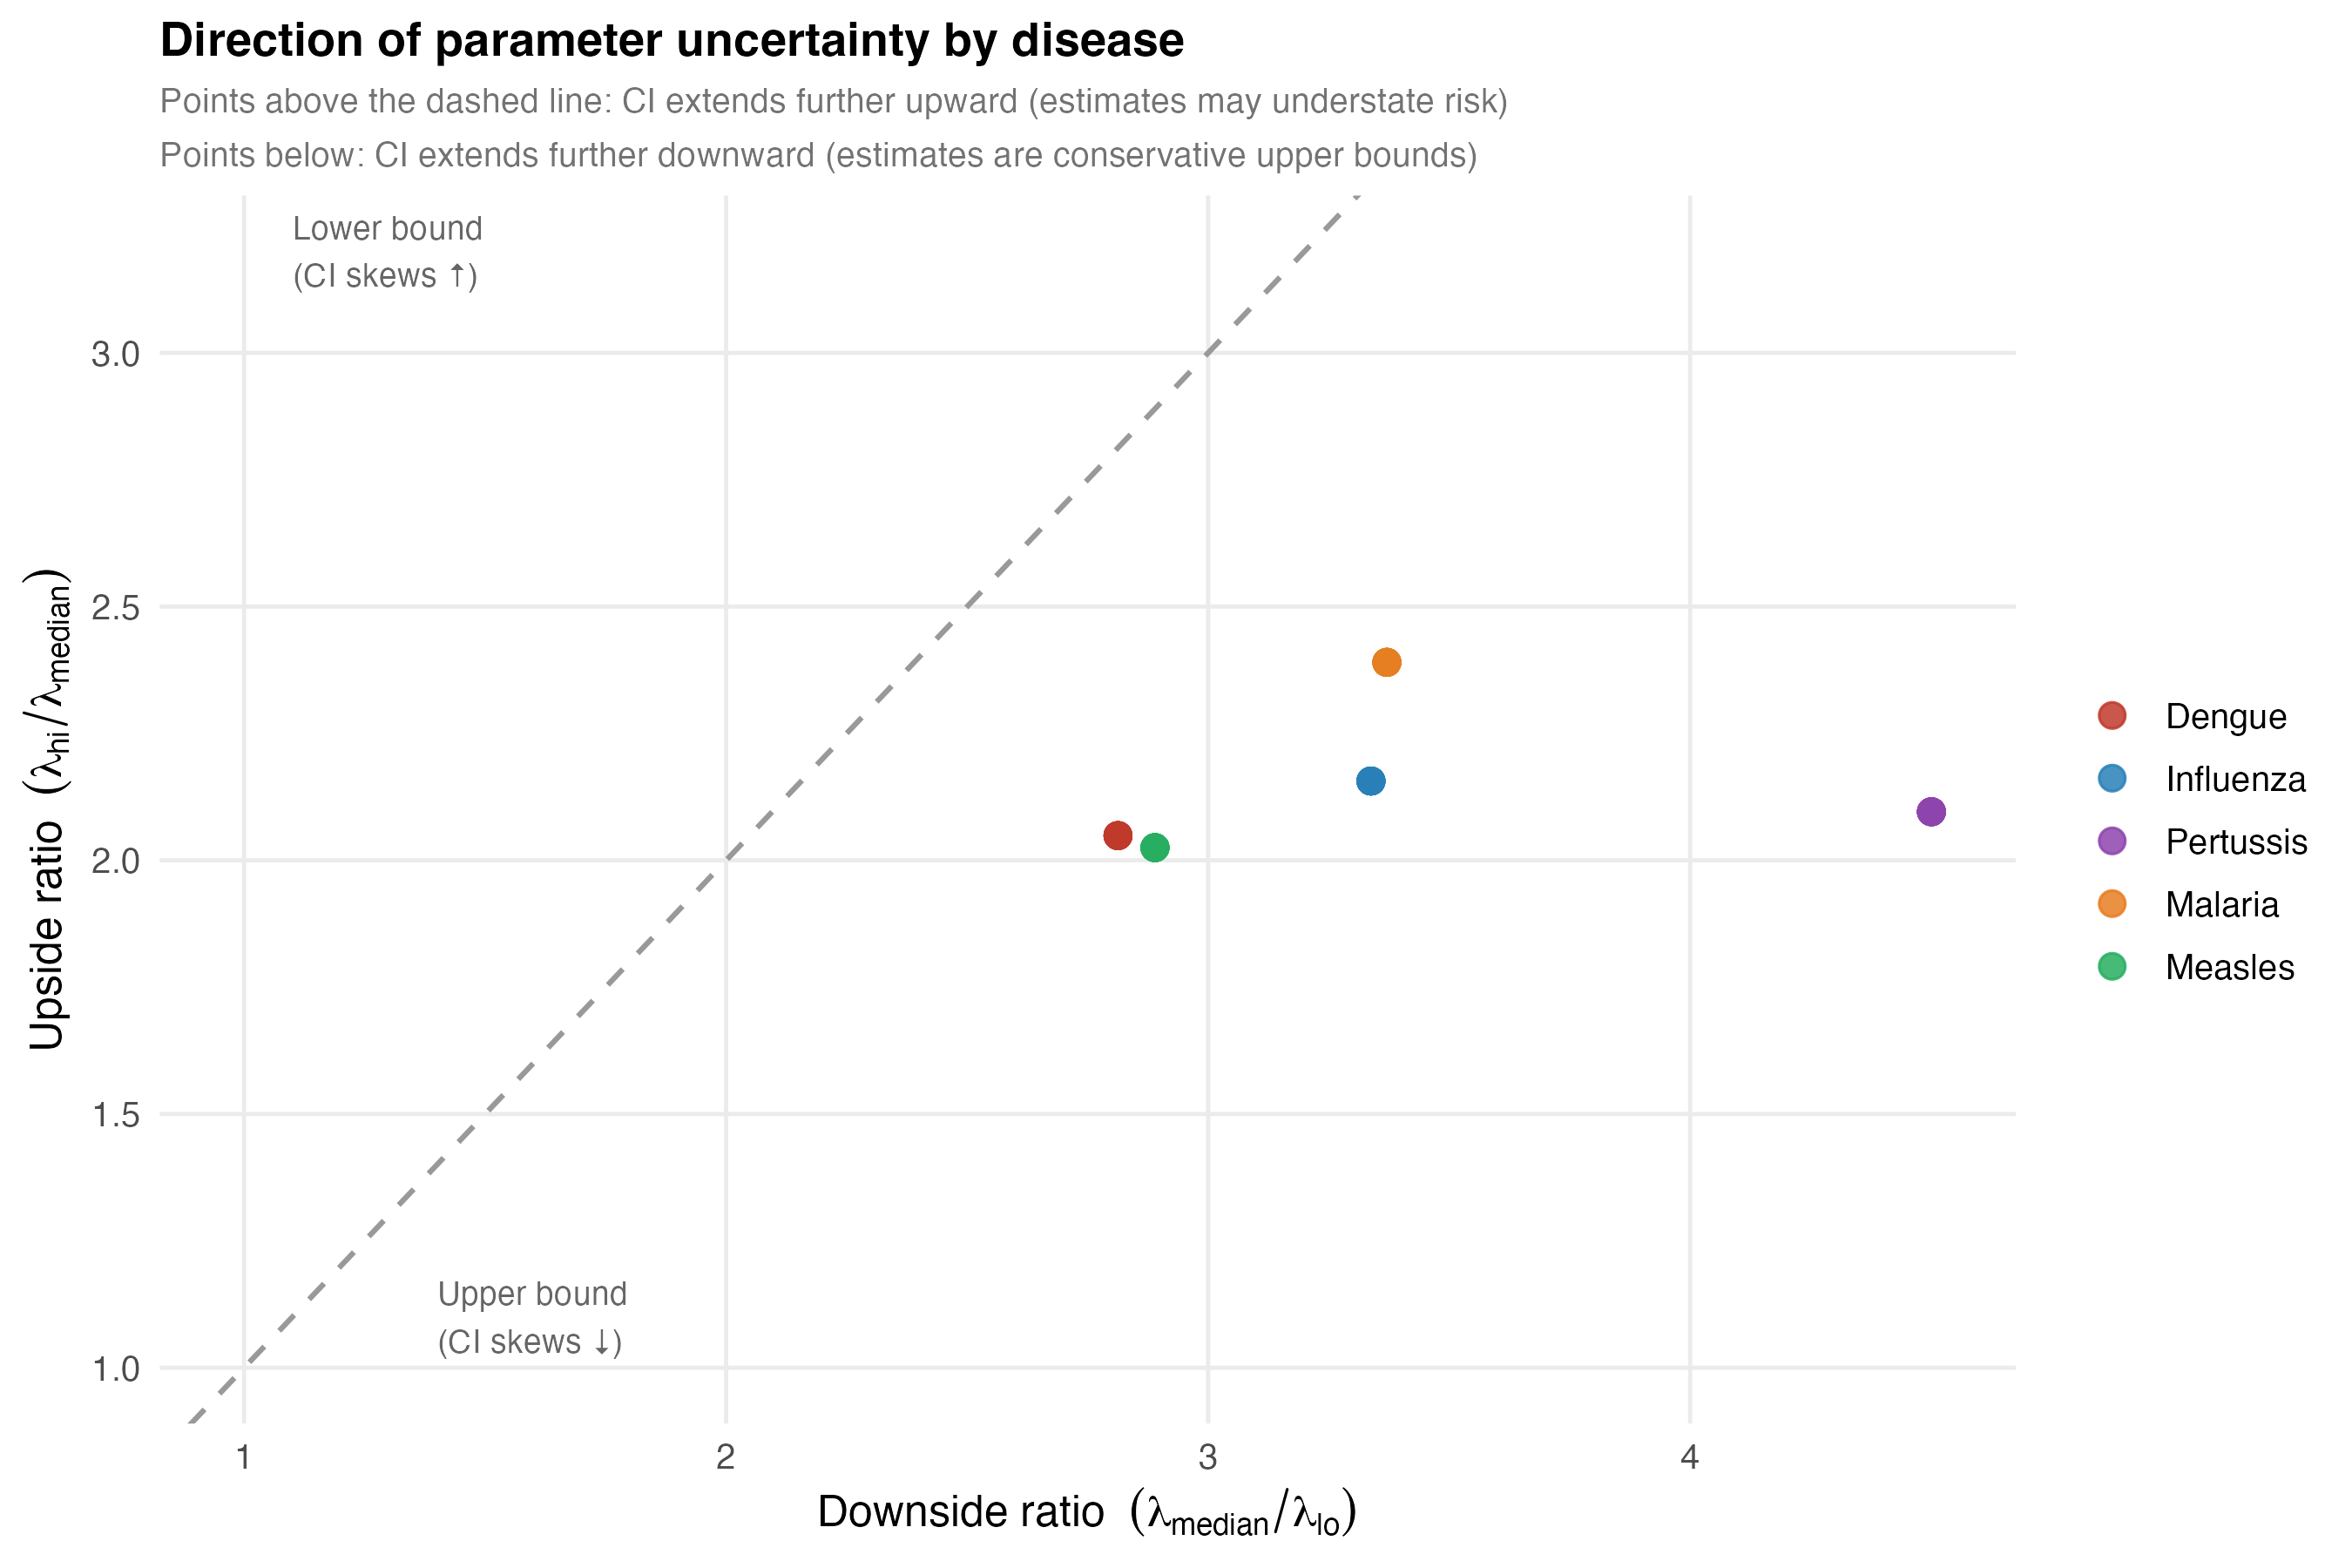
\includegraphics[width=0.8\textwidth]{../Figures/ci_asymmetry.png}
  \caption{Direction of Monte Carlo parameter uncertainty by disease.
    Each point represents one disease--city pair under the schedule-driven
    model. Upside ratio $= \Lambda_\text{hi}/\Lambda_\text{median}$;
    downside ratio $= \Lambda_\text{median}/\Lambda_\text{lo}$.
    Points above the dashed diagonal: CI skews upward (central estimate
    near lower bound of plausible range). Points below: CI skews downward
    (central estimate near upper bound). Dengue and influenza may be
    underestimated; pertussis estimates are conservative upper bounds.}
  \label{fig:ci_asym}
\end{figure}

\subsection*{Importation risk overview: Baseline and WC-adjusted models}

Figures~\ref{fig:heatmap_m1} and~\ref{fig:heatmap_m2} show the same
$P(\geq 1)$ heatmap as Figure~\ref{fig:risk_heatmap} in the main text,
but for the Baseline (Model~1) and WC-adjusted (Model~2) tiers
respectively. City and disease ordering are identical to Figure~\ref{fig:risk_heatmap}
to allow direct visual comparison across all three model tiers.
Dengue importation probability is near-certain ($>0.99$) at the
highest-risk cities under all three models, confirming that this
finding is not an artefact of the schedule-driven travel assumptions.
The step from Model~1 to Model~2 raises probabilities modestly for
most disease--city pairs; the step to Model~3 (main text) introduces
the schedule-based concentration at specific match venues.

\begin{figure}[h!]
  \centering
  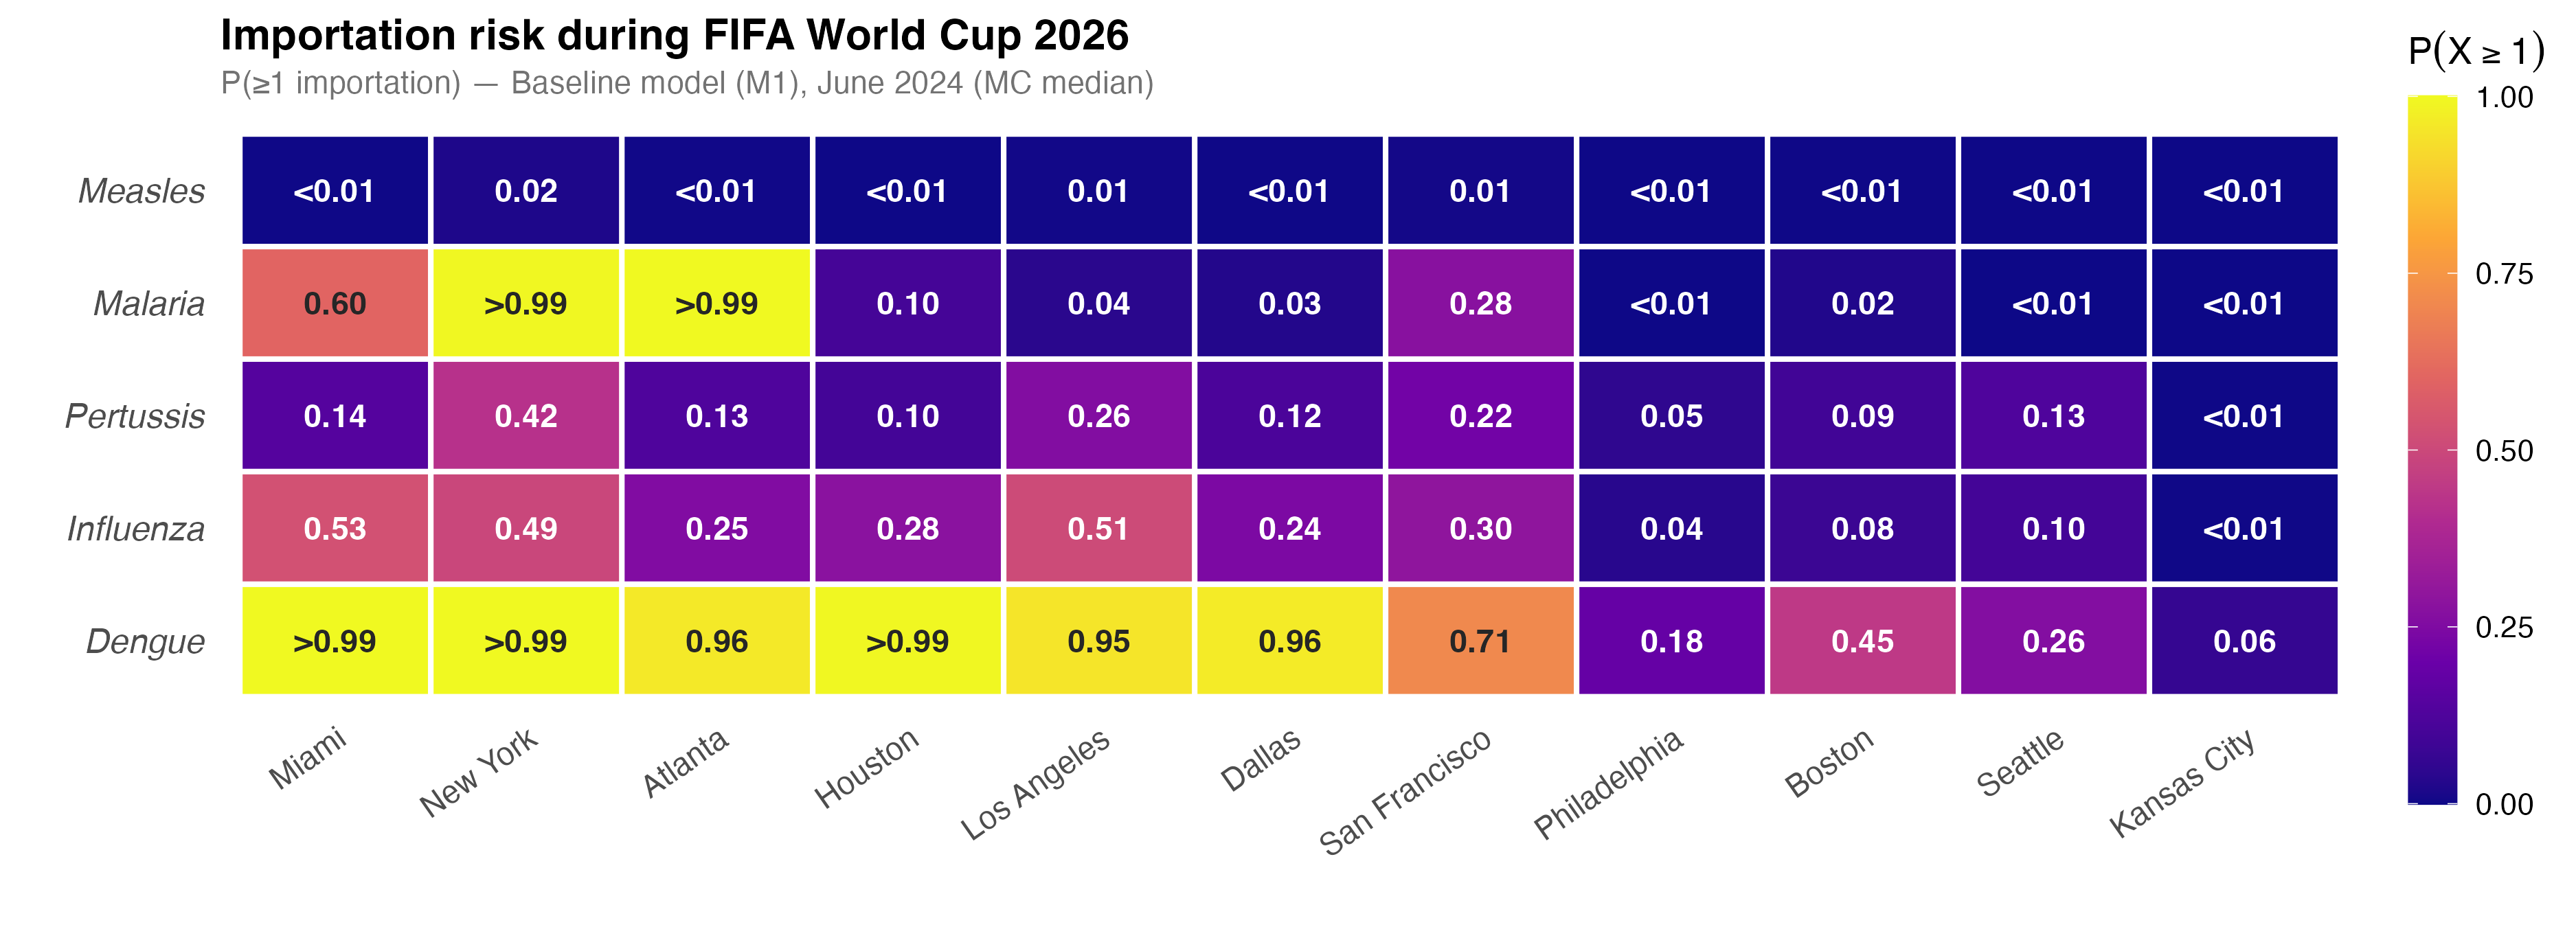
\includegraphics[width=\textwidth]{../Figures/fig1_heatmap_baseline.png}
  \caption{Importation risk overview under the Baseline model (Model~1):
    $P(\geq 1\text{ importation})$ using routine June~2024 COR arrivals
    with no World Cup growth adjustment (MC median, 5,000 draws).
    Same city and disease ordering as Figure~\ref{fig:risk_heatmap}.}
  \label{fig:heatmap_m1}
\end{figure}

\begin{figure}[h!]
  \centering
  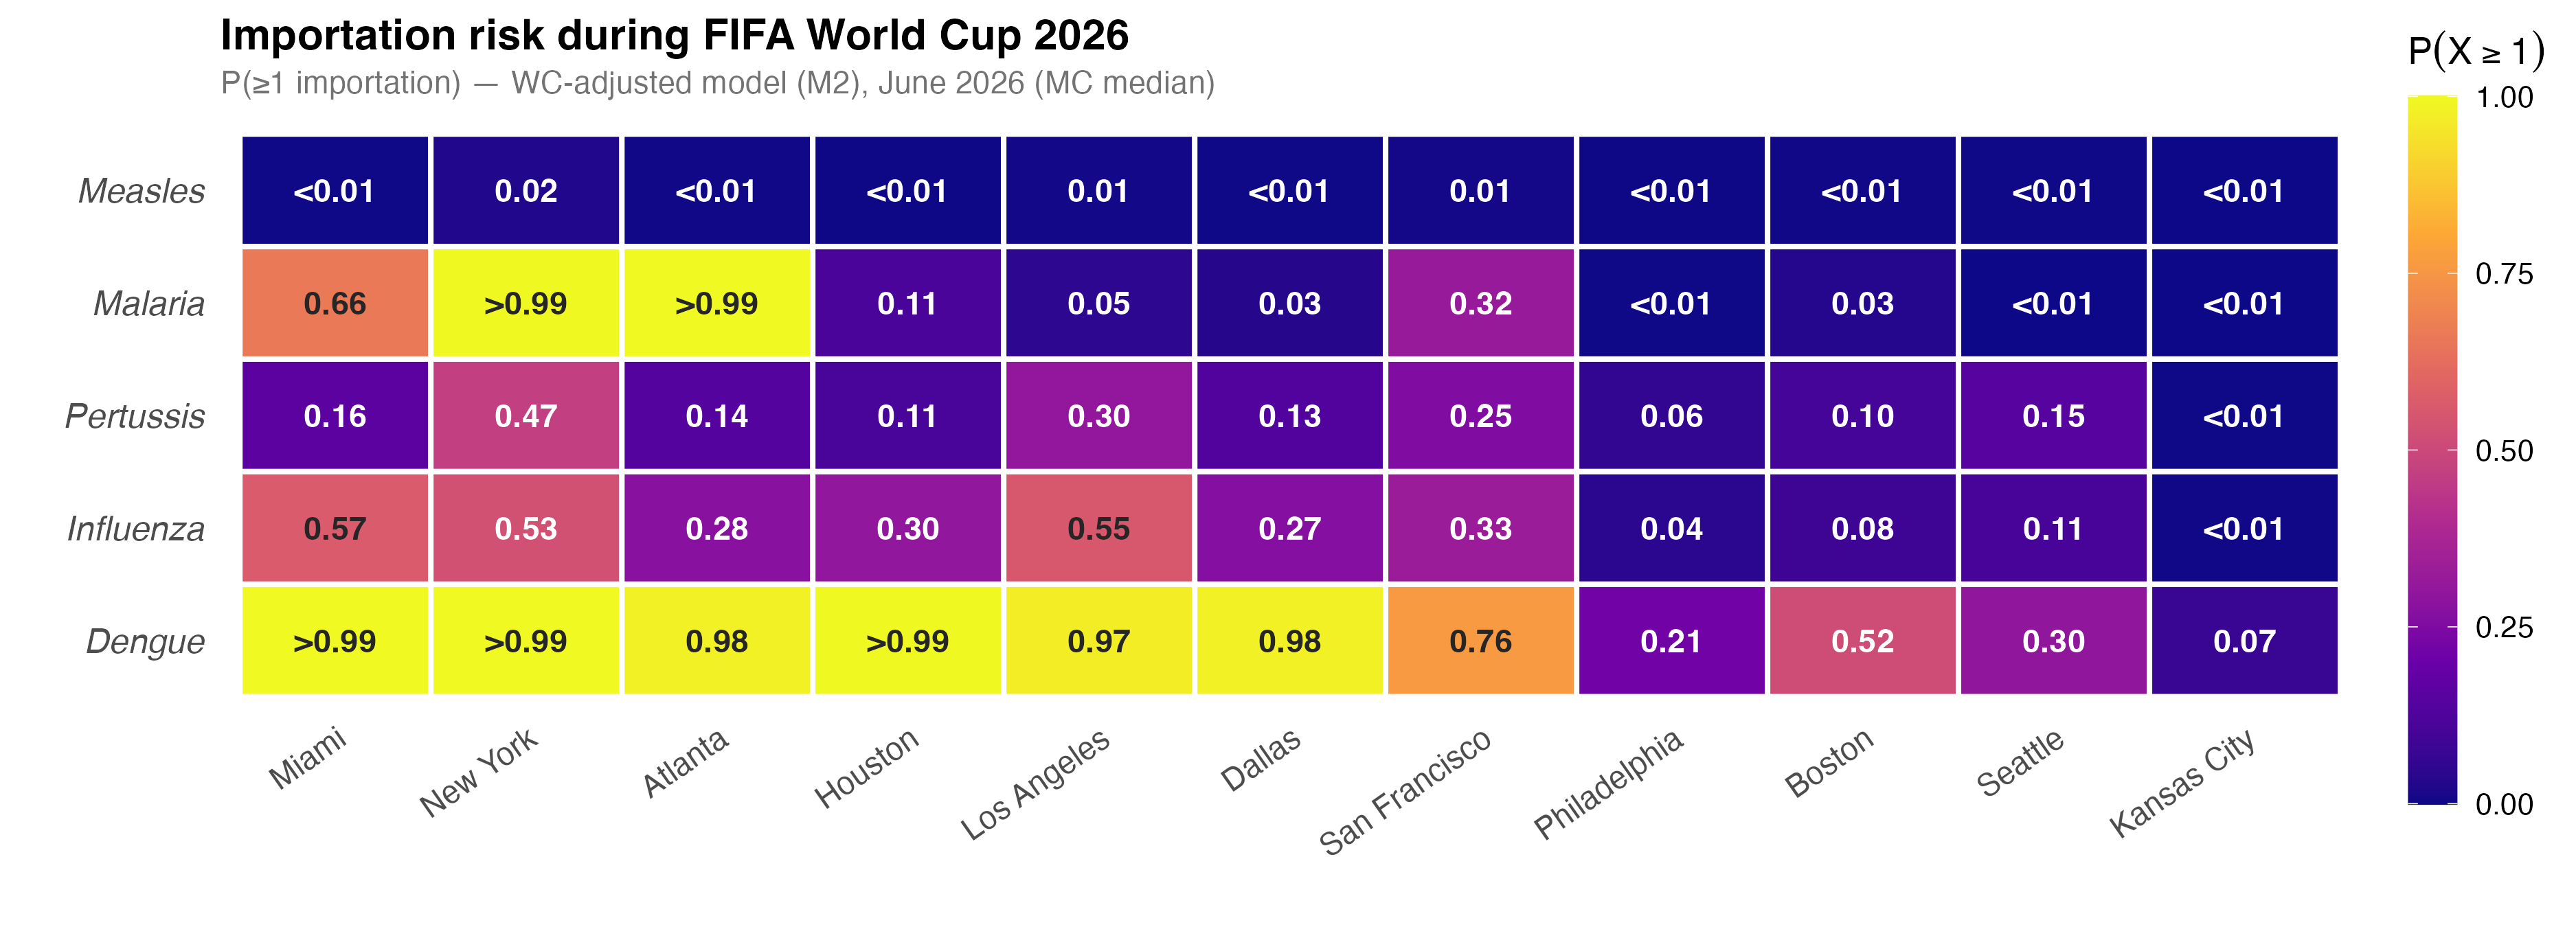
\includegraphics[width=\textwidth]{../Figures/fig1_heatmap_wc.png}
  \caption{Importation risk overview under the WC-adjusted model (Model~2):
    $P(\geq 1\text{ importation})$ using June~2026 projected arrivals
    scaled by NTTO growth factors (MC median, 5,000 draws).
    Same city and disease ordering as Figure~\ref{fig:risk_heatmap}.}
  \label{fig:heatmap_m2}
\end{figure}

\subsection*{Dengue stream decomposition by source country}

Figure~\ref{fig:stream_dengue} shows the dengue-specific travel
stream decomposition for the top~20 source countries: background
travel (blue) vs.\ WC fans (orange). The full five-disease stream
panel is Figure~\ref{fig:stream_panel}.

\begin{figure}[h!]
  \centering
  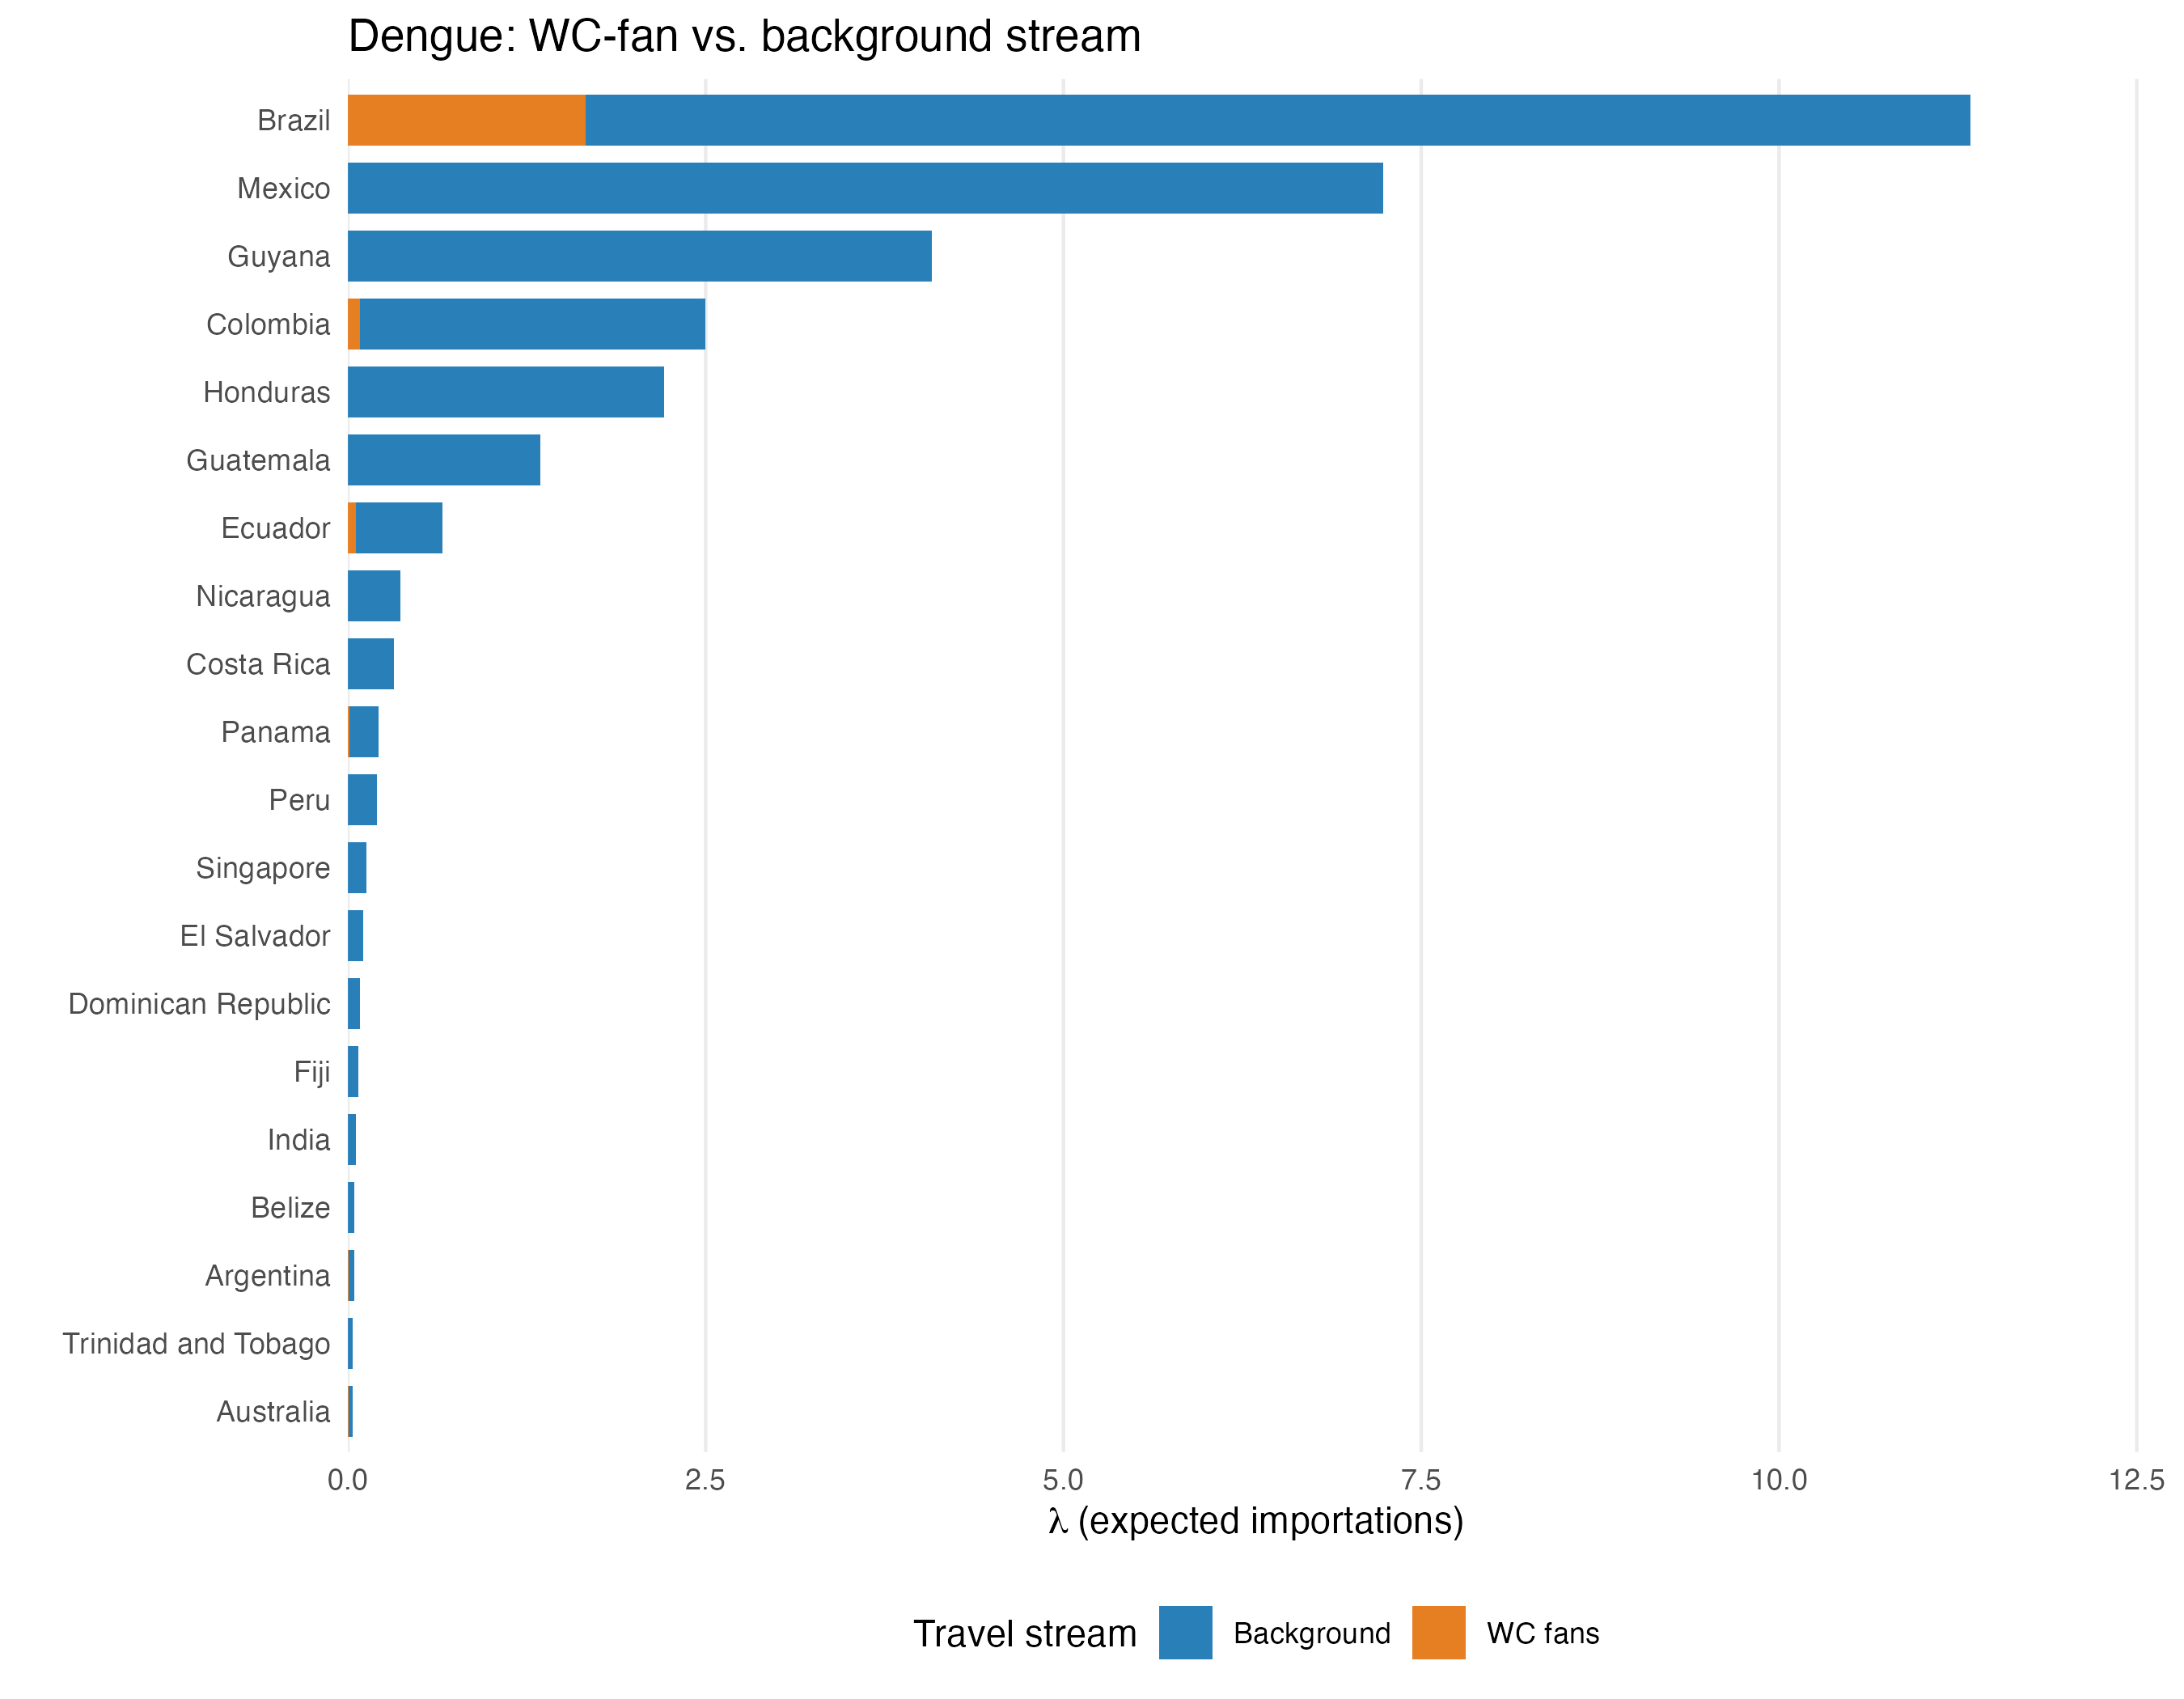
\includegraphics[width=0.85\textwidth]{../Figures/stream_breakdown_dengue.png}
  \caption{Dengue: importation intensity by travel stream for the
    top~20 source countries. Blue = background travel; orange = WC fans.
    Background dominates for all countries; the WC fan increment is
    largest for high-incidence WC-qualified nations
    (Brazil, Colombia, Ecuador).}
  \label{fig:stream_dengue}
\end{figure}

\subsection*{WC-fan vs.\ background travel stream decomposition}

Figure~\ref{fig:stream_panel} decomposes the top 20 contributing
countries by travel stream (WC fans vs.\ background) for each of
the five diseases. For WC-qualified countries, the WC-fan stream
contributes a meaningful but typically minority share of the total
importation intensity, consistent with the $\approx 8.3\%$ fan
fraction derived from the growth factor decomposition. Countries with
the largest WC fan contributions are those that (1) have a qualified
team, (2) have high disease incidence, and (3) have their team's
matches concentrated at a small number of venue cities, increasing
the local fan density at those venues.

Non-qualified countries, regardless of their disease burden,
contribute exclusively through the background stream; their presence
in the top 20 reflects high June travel volumes to the United States
rather than any WC-specific effect. This decomposition highlights
that the background stream dominates total importation risk for most
source countries: the WC tournament amplifies risk at specific cities
and for specific diseases, but baseline travel patterns set the
underlying risk floor across all cities and diseases.

\begin{figure}[h!]
  \centering
  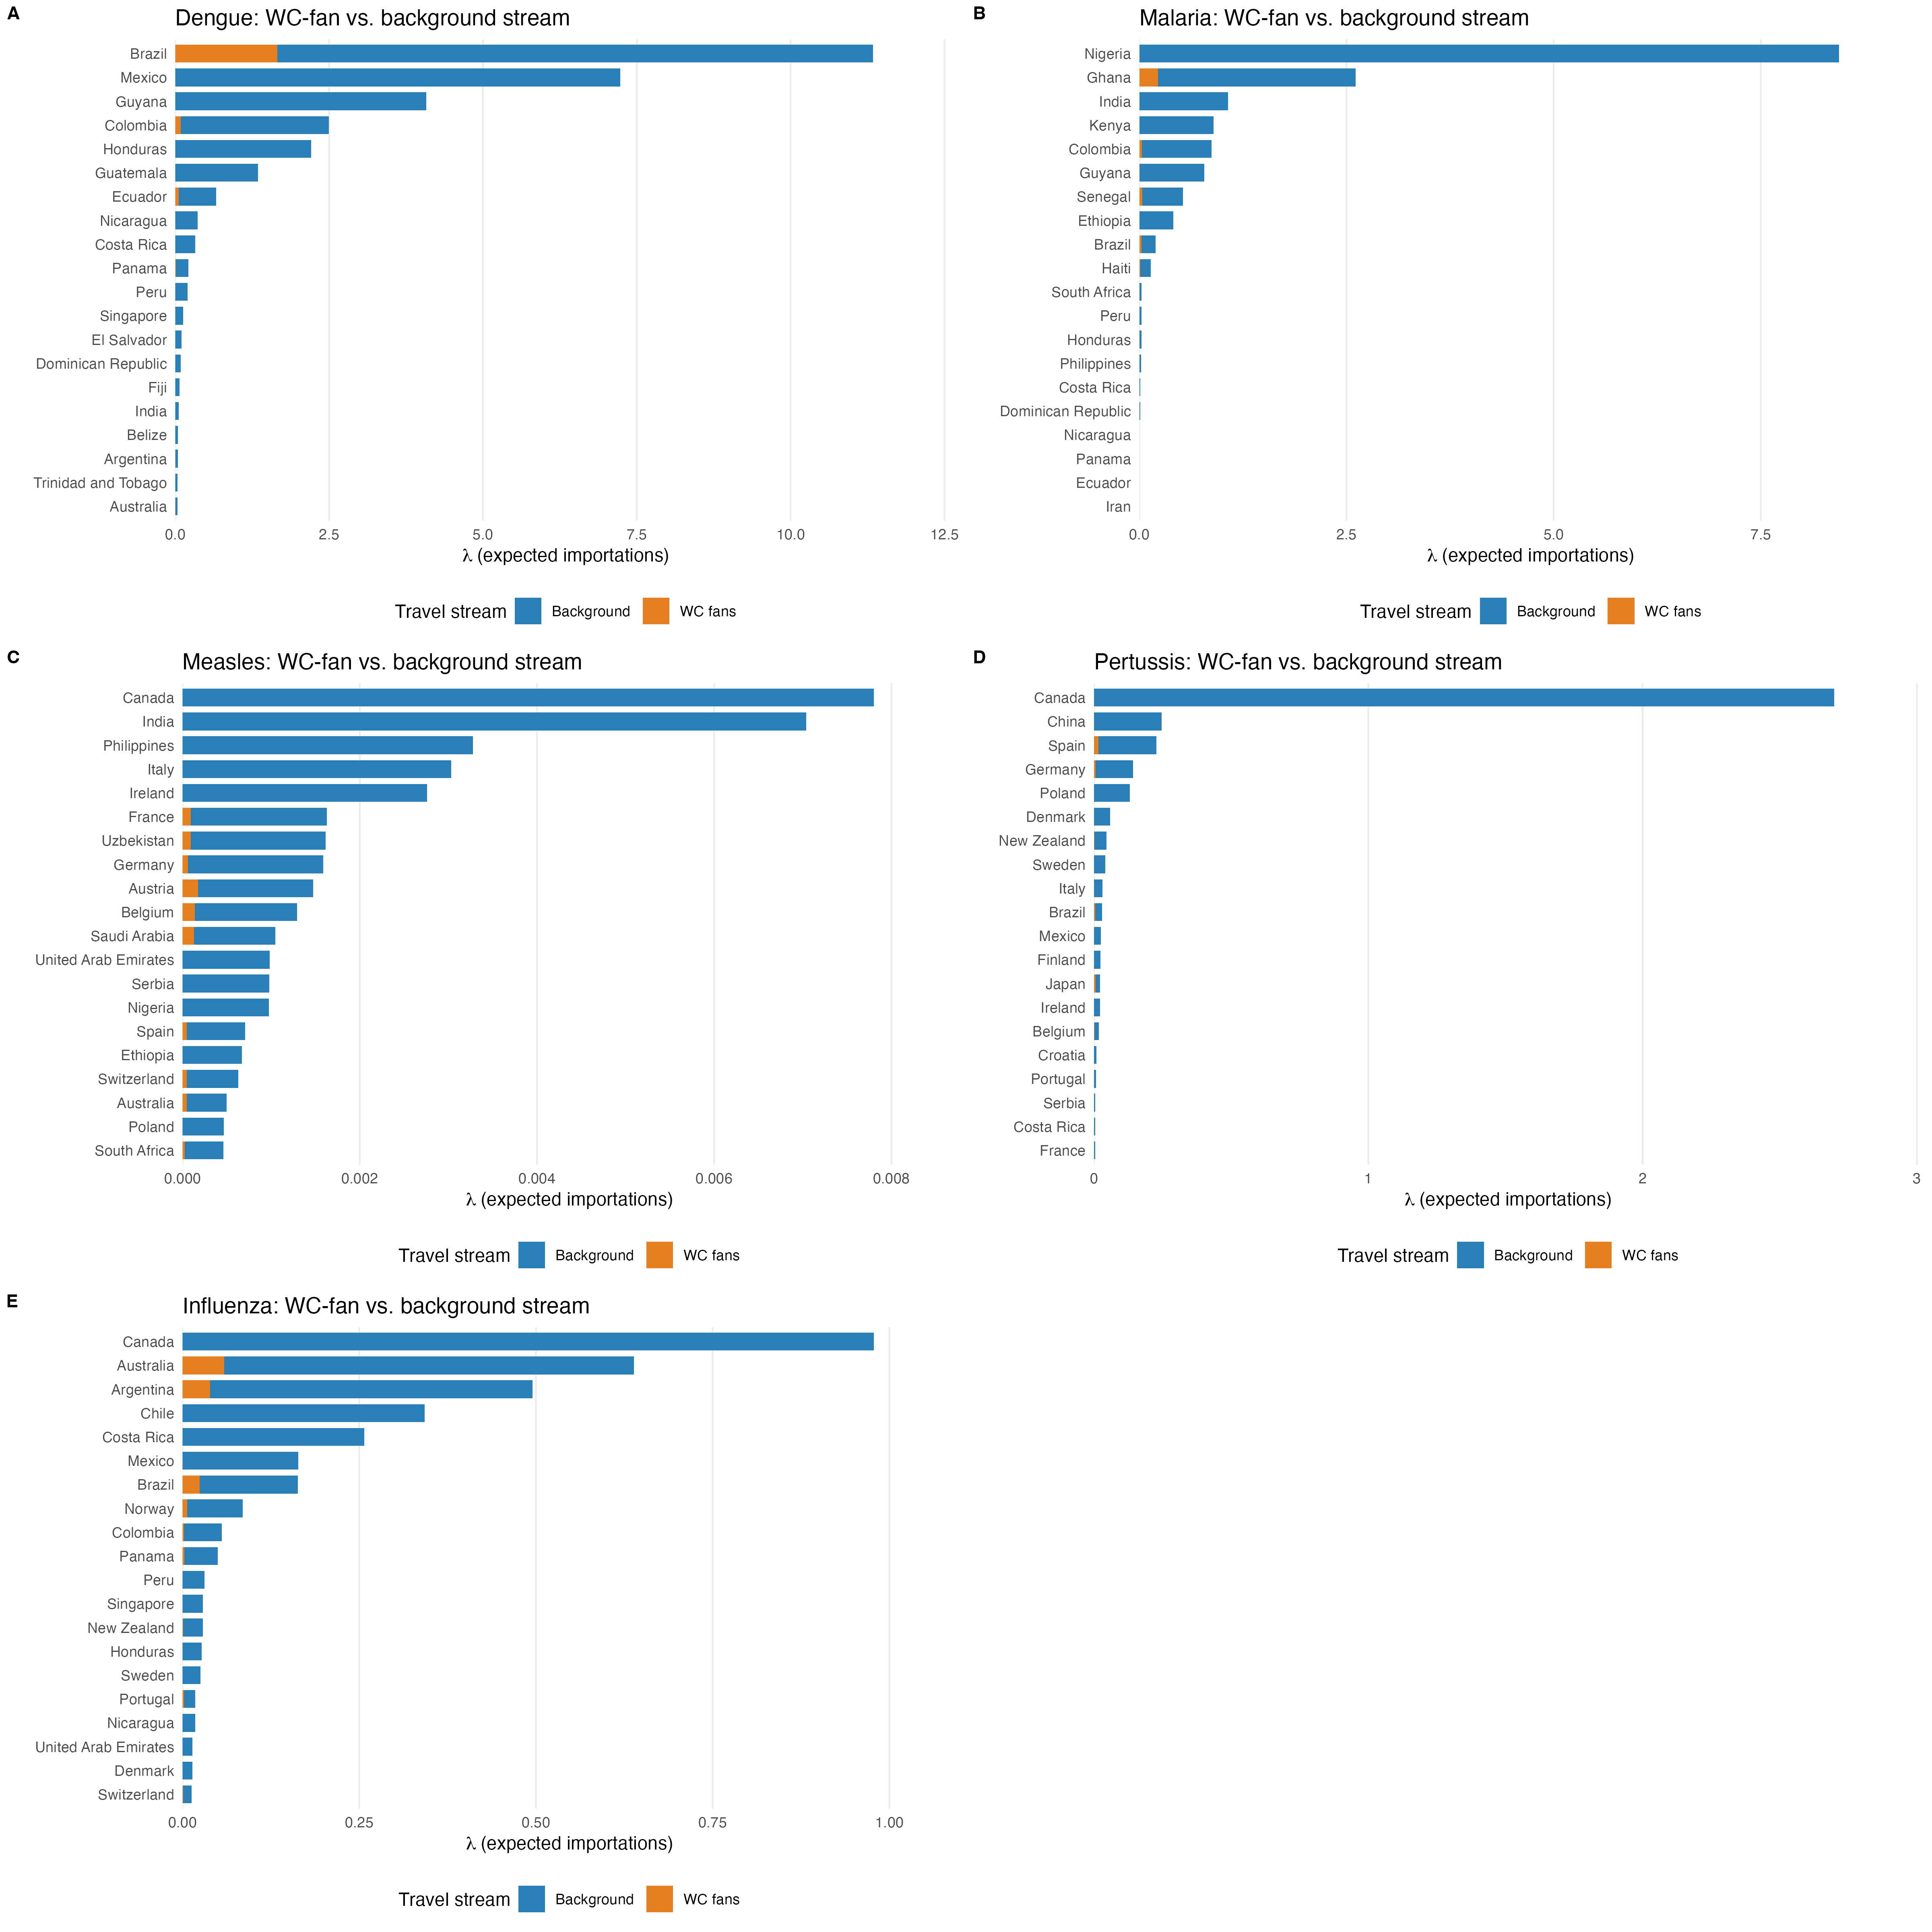
\includegraphics[width=\textwidth]{../Figures/stream_breakdown_panel.png}
  \caption{WC-fan vs.\ background travel stream decomposition for the
    top 20 source countries by total importation intensity, for each
    of the five diseases. \textcolor{orange!80!black}{Orange} = WC fans;
    \textcolor{blue!70!black}{Blue} = background. Countries with WC
    teams show a non-zero WC-fan component; non-qualified countries
    contribute only through background travel.}
  \label{fig:stream_panel}
\end{figure}

\subsection*{Country $\times$ city importation heatmaps}

Figures~\ref{fig:heatmap_dengue}--\ref{fig:heatmap_influenza} present
the country $\times$ city importation matrix ($\lambda_{c,v,d}$)
for each disease. The heatmaps reveal a consistent spatial pattern:
WC-qualified countries from high-incidence regions show importation
concentrated at the venue cities where their team plays, producing a
block-diagonal structure aligned with the match schedule. Non-qualified
countries show importation spread more diffusely across cities in
proportion to T-100 routing fractions, reflecting their reliance on
normal tourist routing patterns.

For dengue (Figure~\ref{fig:heatmap_dengue}), the highest
country--city cells correspond to Latin American WC teams (Brazil,
Colombia, Ecuador, Paraguay, Uruguay, Argentina) at their respective
match venues. Miami, Houston, and Los Angeles receive notable dengue
contributions from multiple Latin American and Caribbean source
countries through both the WC-fan and background streams. For malaria
(Figure~\ref{fig:heatmap_malaria}), the risk matrix is sparser, with
high values concentrated in West African nations at their match venues
and lower diffuse contributions elsewhere.

Measles (Figure~\ref{fig:heatmap_measles}) shows a distinct pattern
from dengue and malaria: despite having the highest $\rho$ value,
the low $p_d$ suppresses absolute importation intensities across all
country--city pairs, resulting in a more uniformly low-intensity
matrix with a few notable peaks at cities hosting matches for countries
with documented measles outbreaks. Pertussis
(Figure~\ref{fig:heatmap_pertussis}) shows the broadest geographic
spread, consistent with its global endemicity and high $p_d$; the
matrix includes non-trivial values from European and East Asian
countries in addition to Latin American ones.

\begin{figure}[h!]
  \centering
  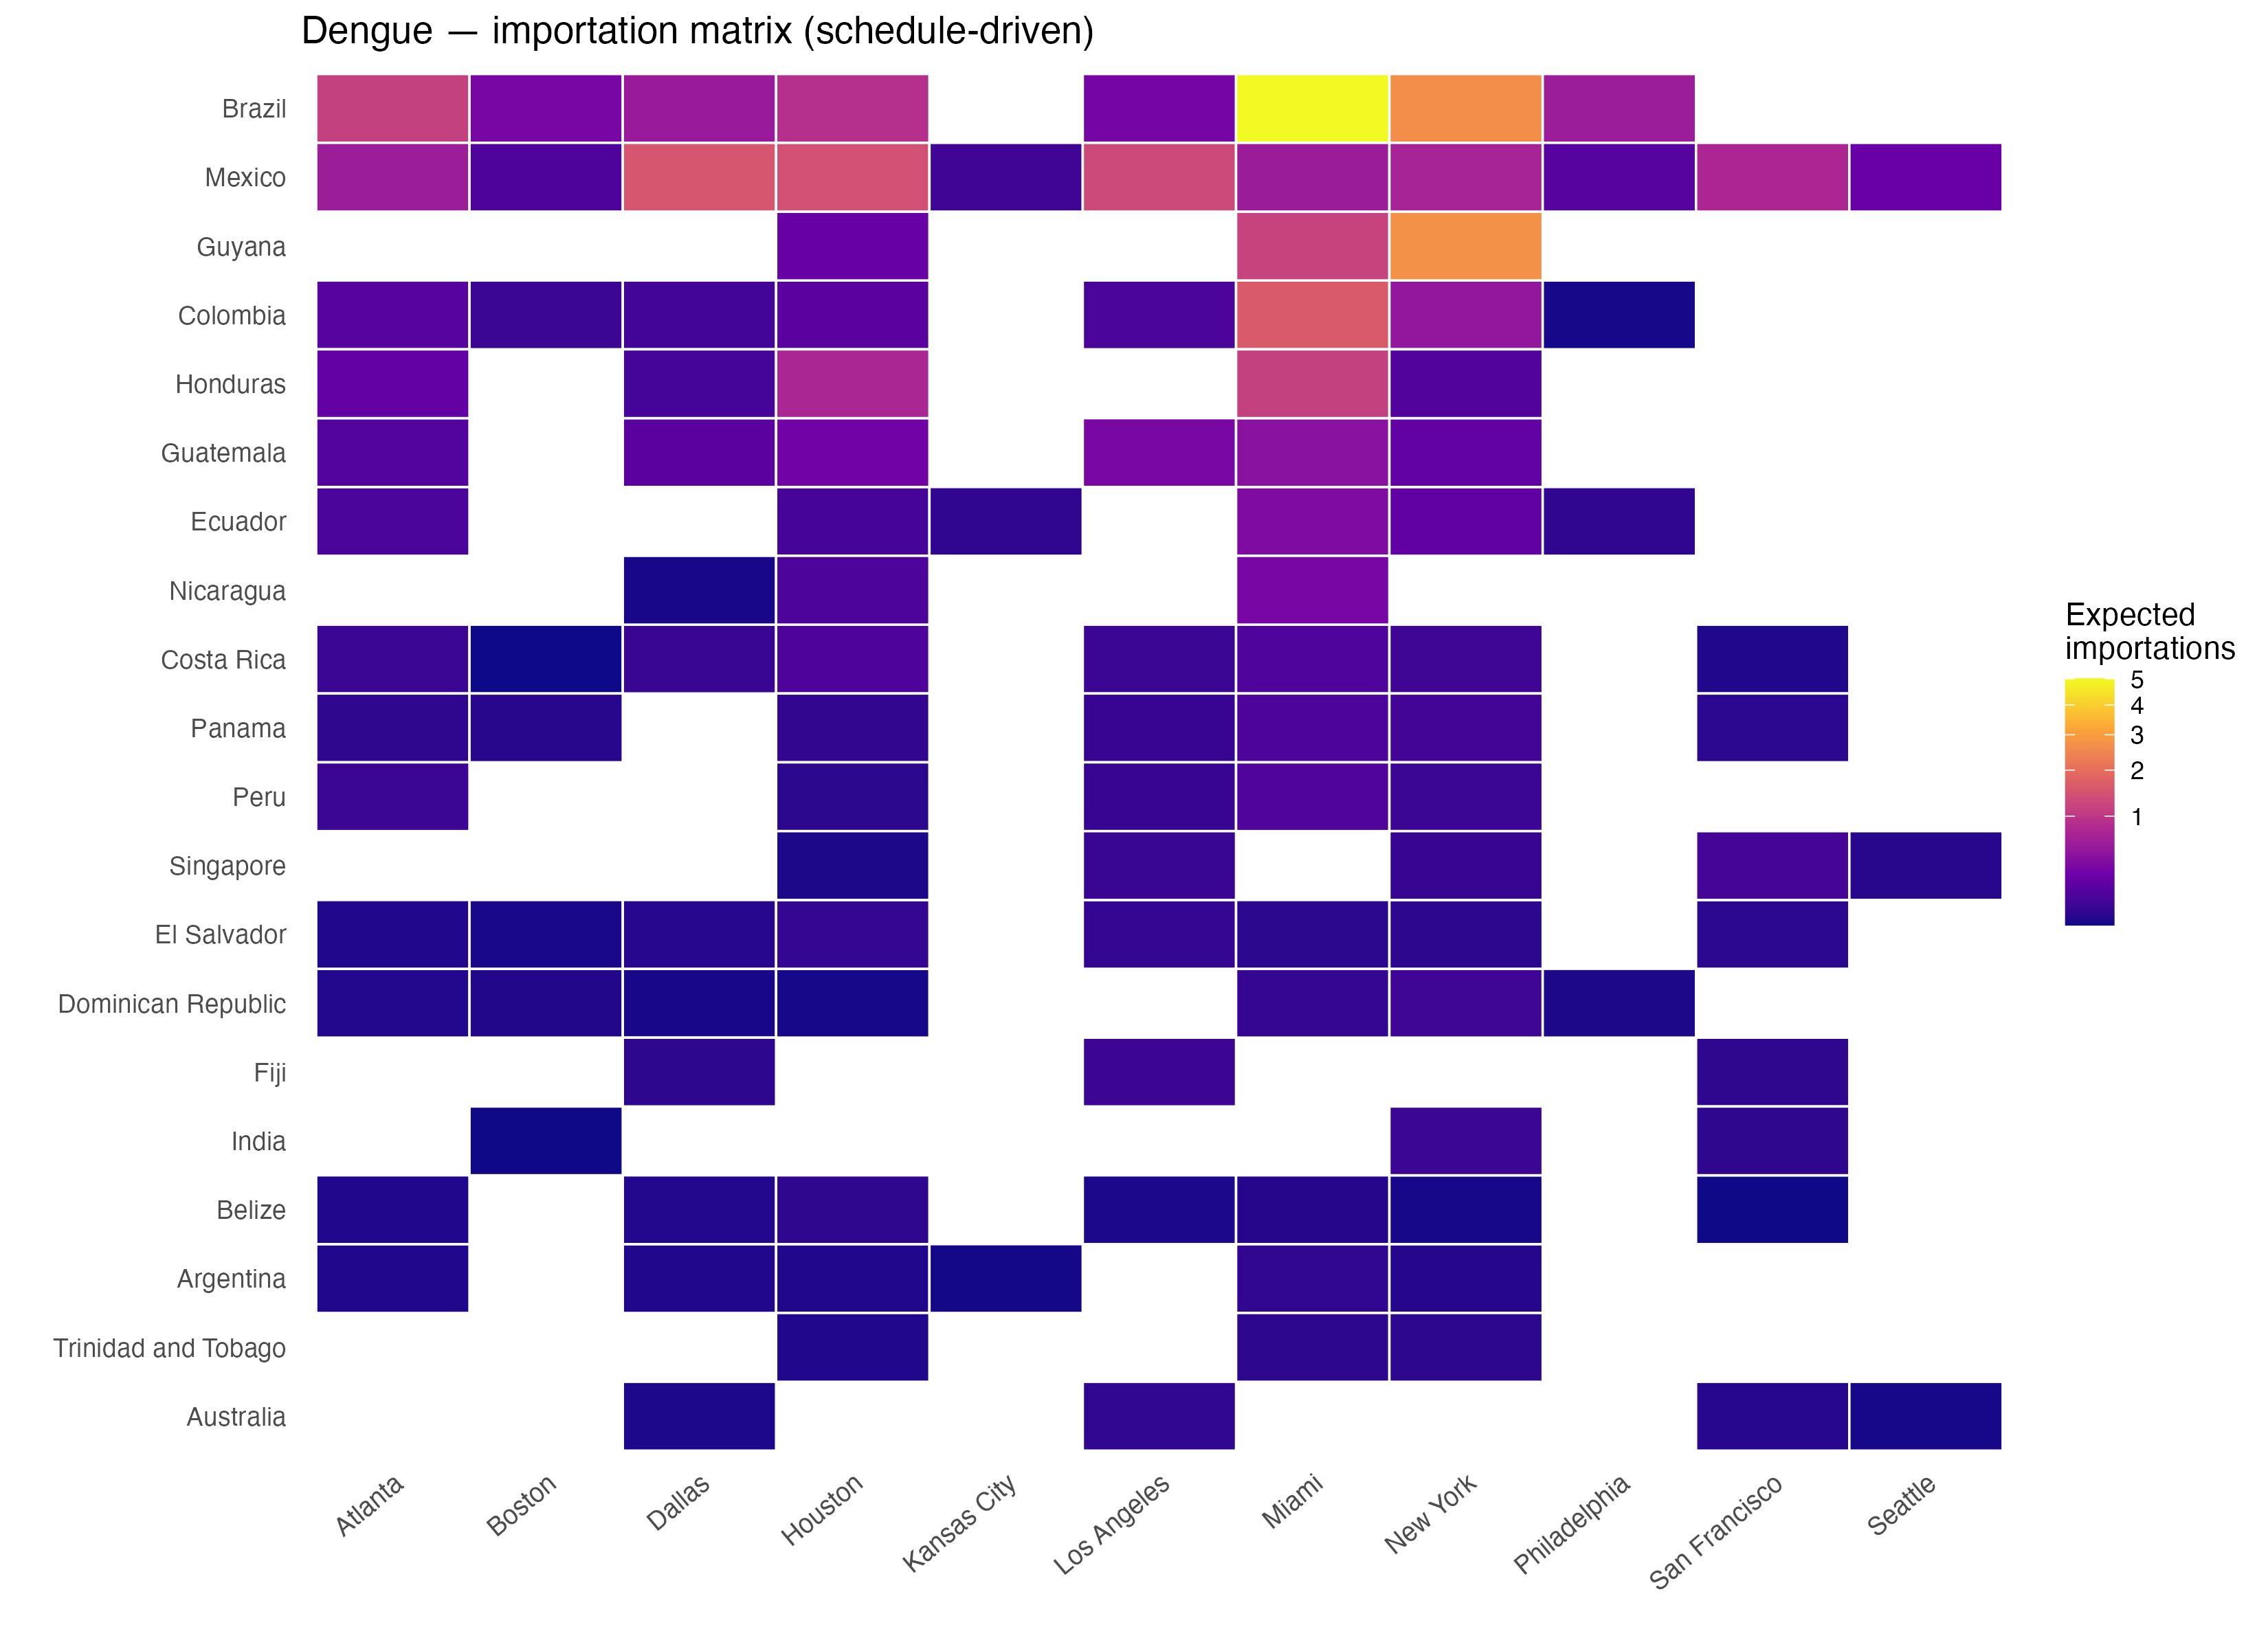
\includegraphics[width=\textwidth]{../Figures/heatmap_dengue.png}
  \caption{Dengue importation matrix: expected importations
    $\lambda_{c,v}$ by source country (rows, ordered by total burden)
    and destination city (columns) under the schedule-driven model.
    Plasma colour scale: bright yellow/orange = high expected
    importations; dark purple/blue = low.}
  \label{fig:heatmap_dengue}
\end{figure}

\begin{figure}[h!]
  \centering
  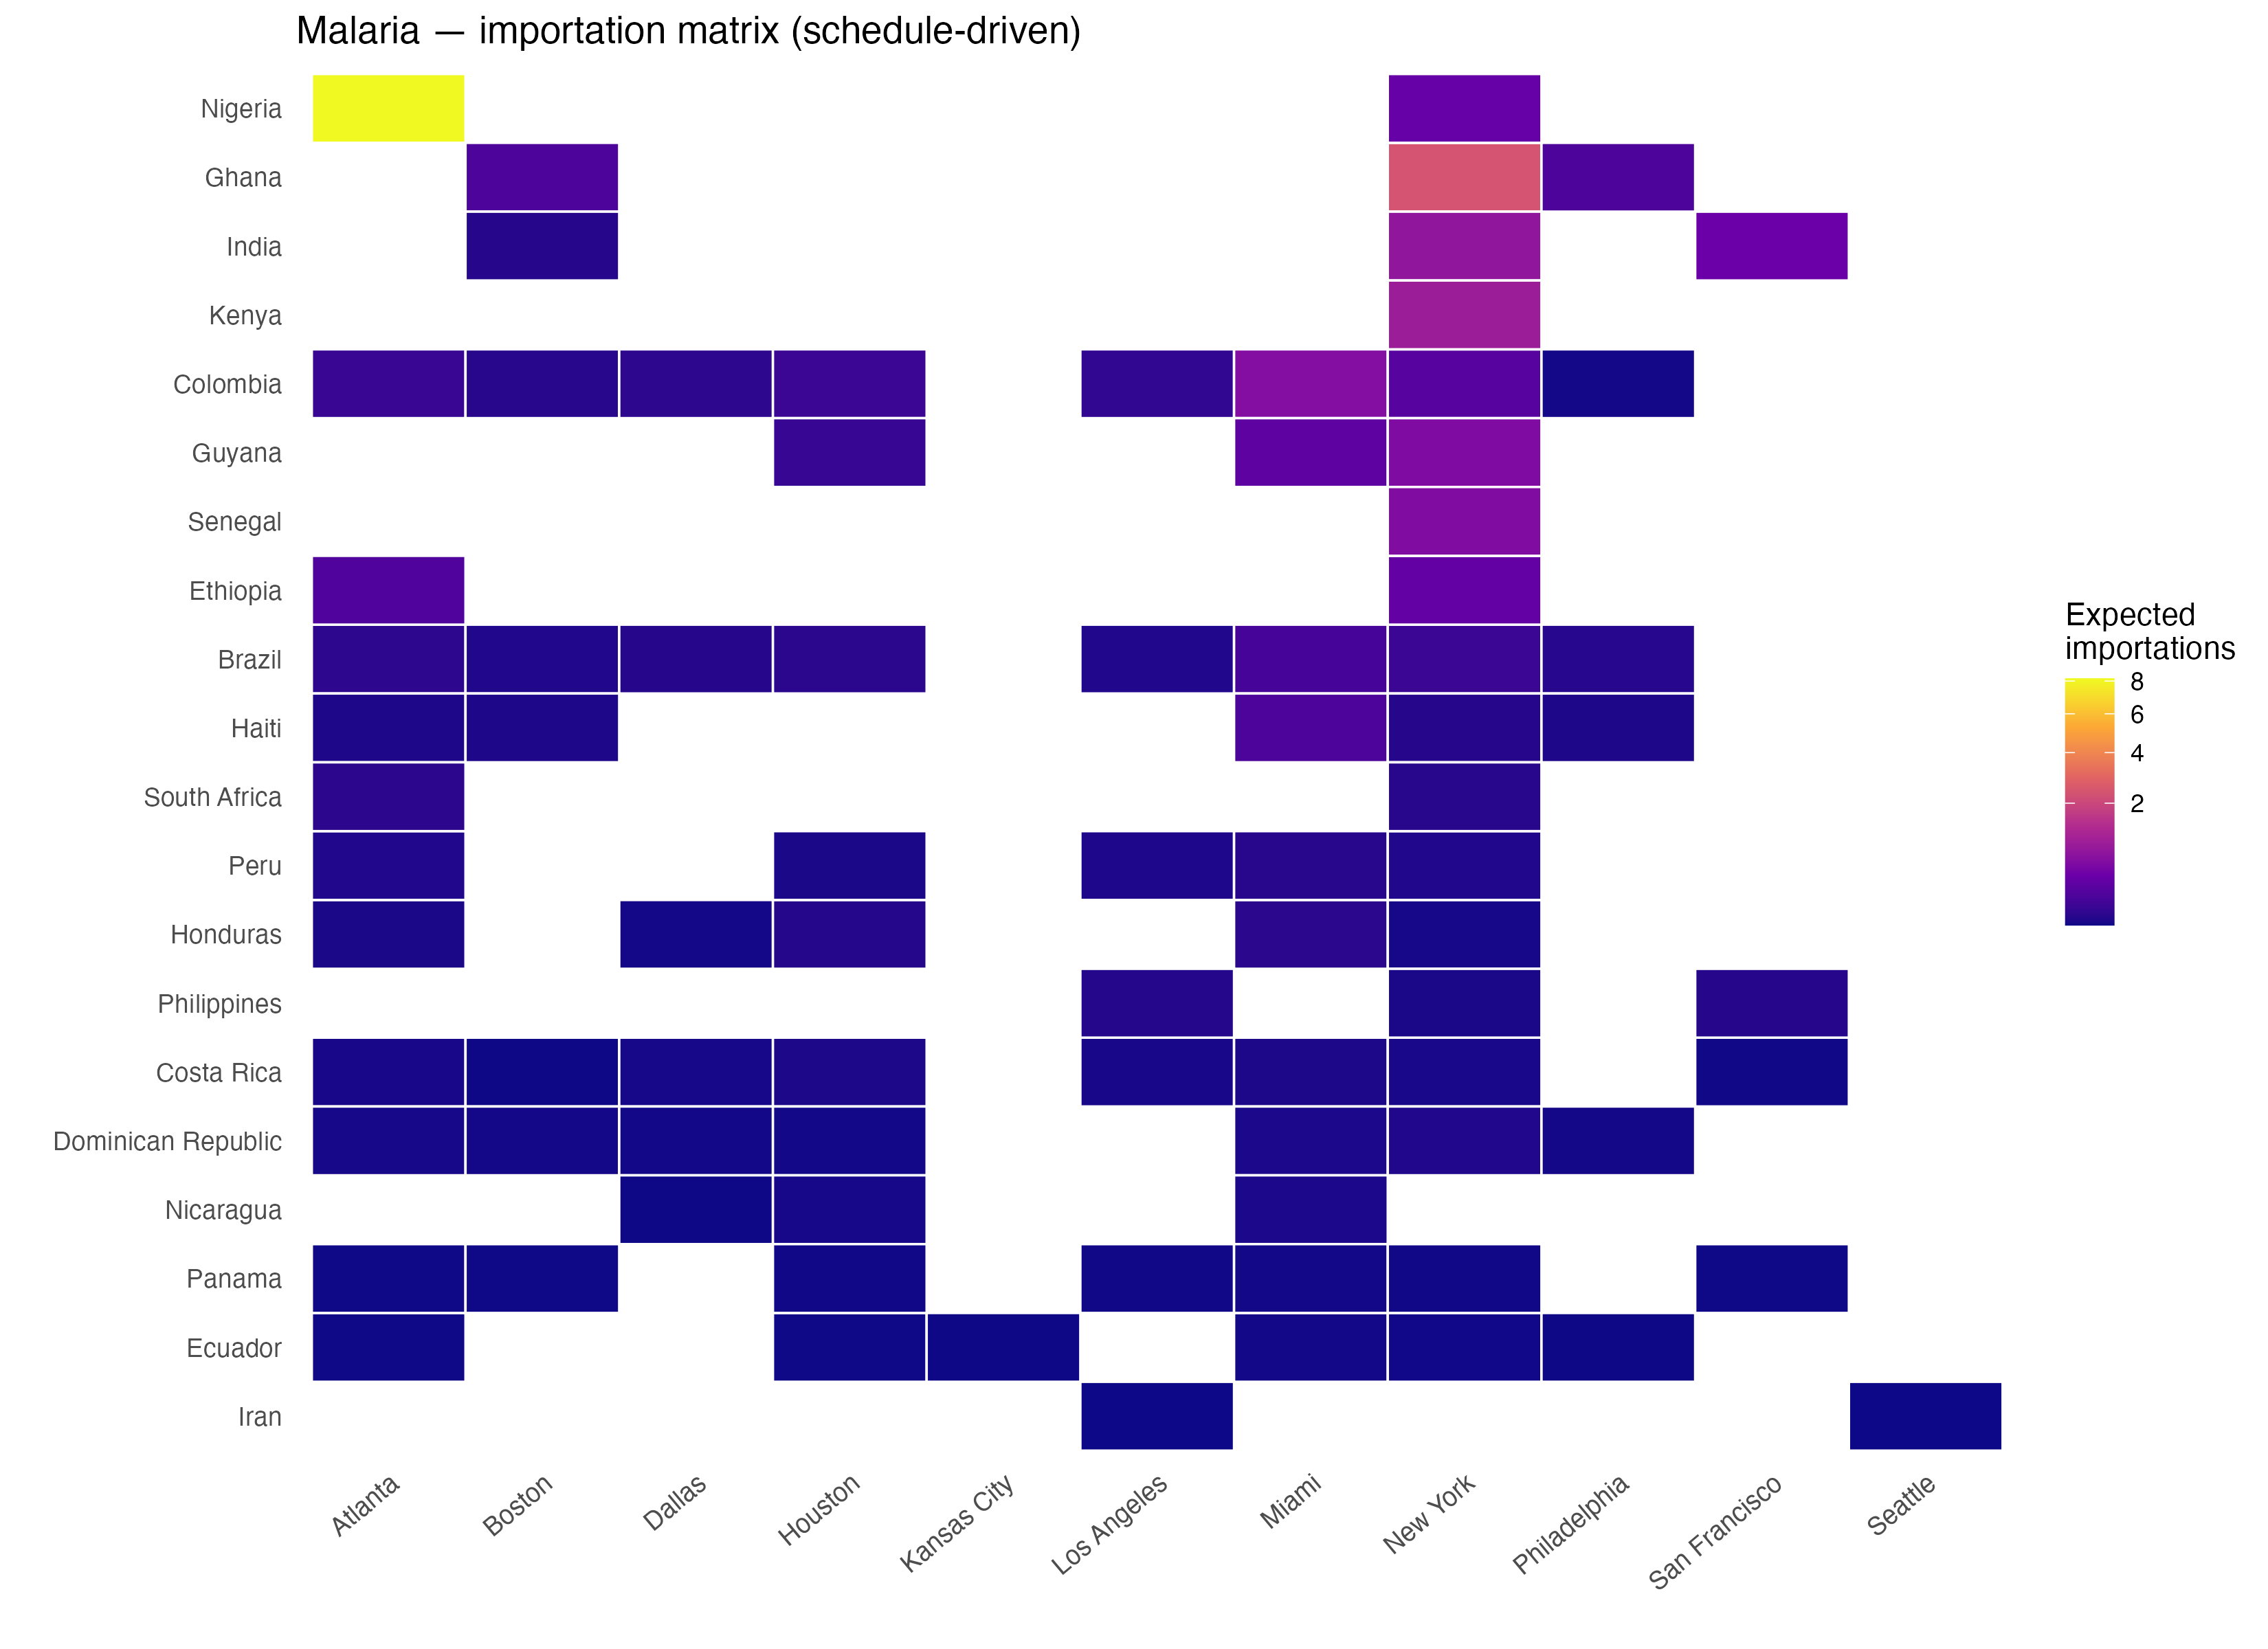
\includegraphics[width=\textwidth]{../Figures/heatmap_malaria.png}
  \caption{Malaria importation matrix. Same structure as
    Figure~\ref{fig:heatmap_dengue}. Risk is concentrated in West
    and Central African source countries.}
  \label{fig:heatmap_malaria}
\end{figure}

\begin{figure}[h!]
  \centering
  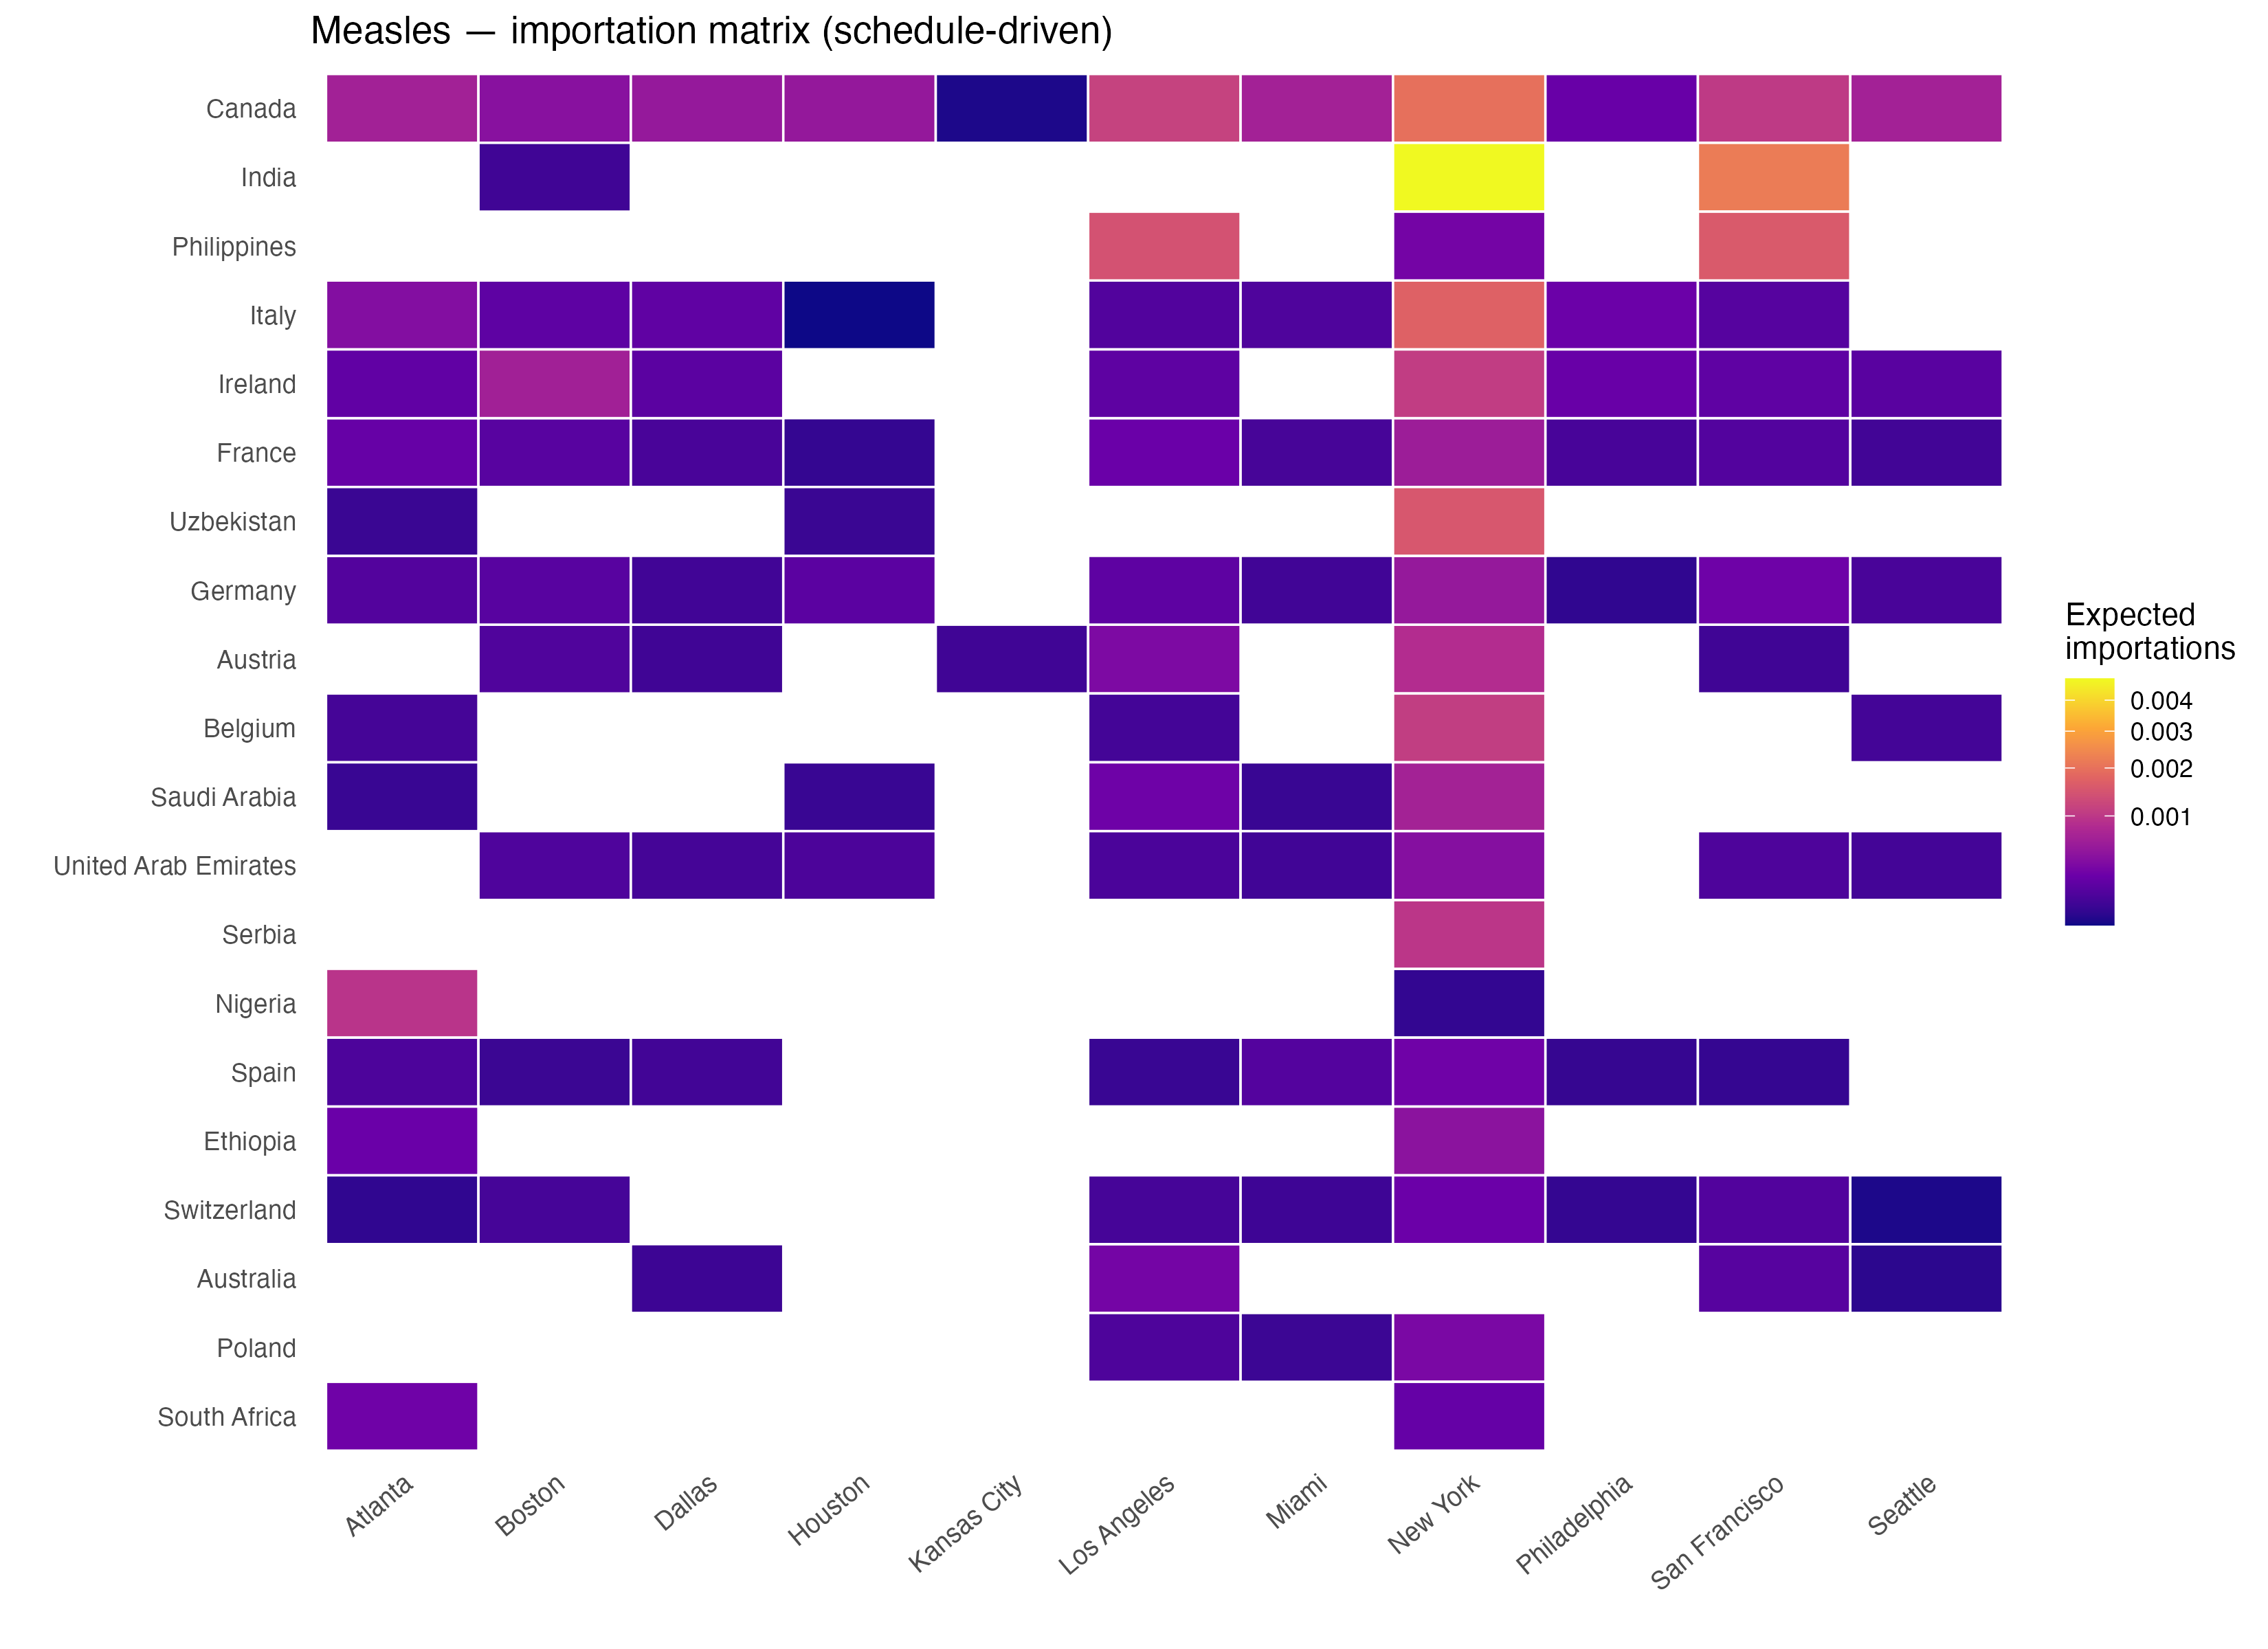
\includegraphics[width=\textwidth]{../Figures/heatmap_measles.png}
  \caption{Measles importation matrix. Low absolute intensities
    across all cells reflect the low travel-while-infectious
    probability ($p = 0.05$).}
  \label{fig:heatmap_measles}
\end{figure}

\begin{figure}[h!]
  \centering
  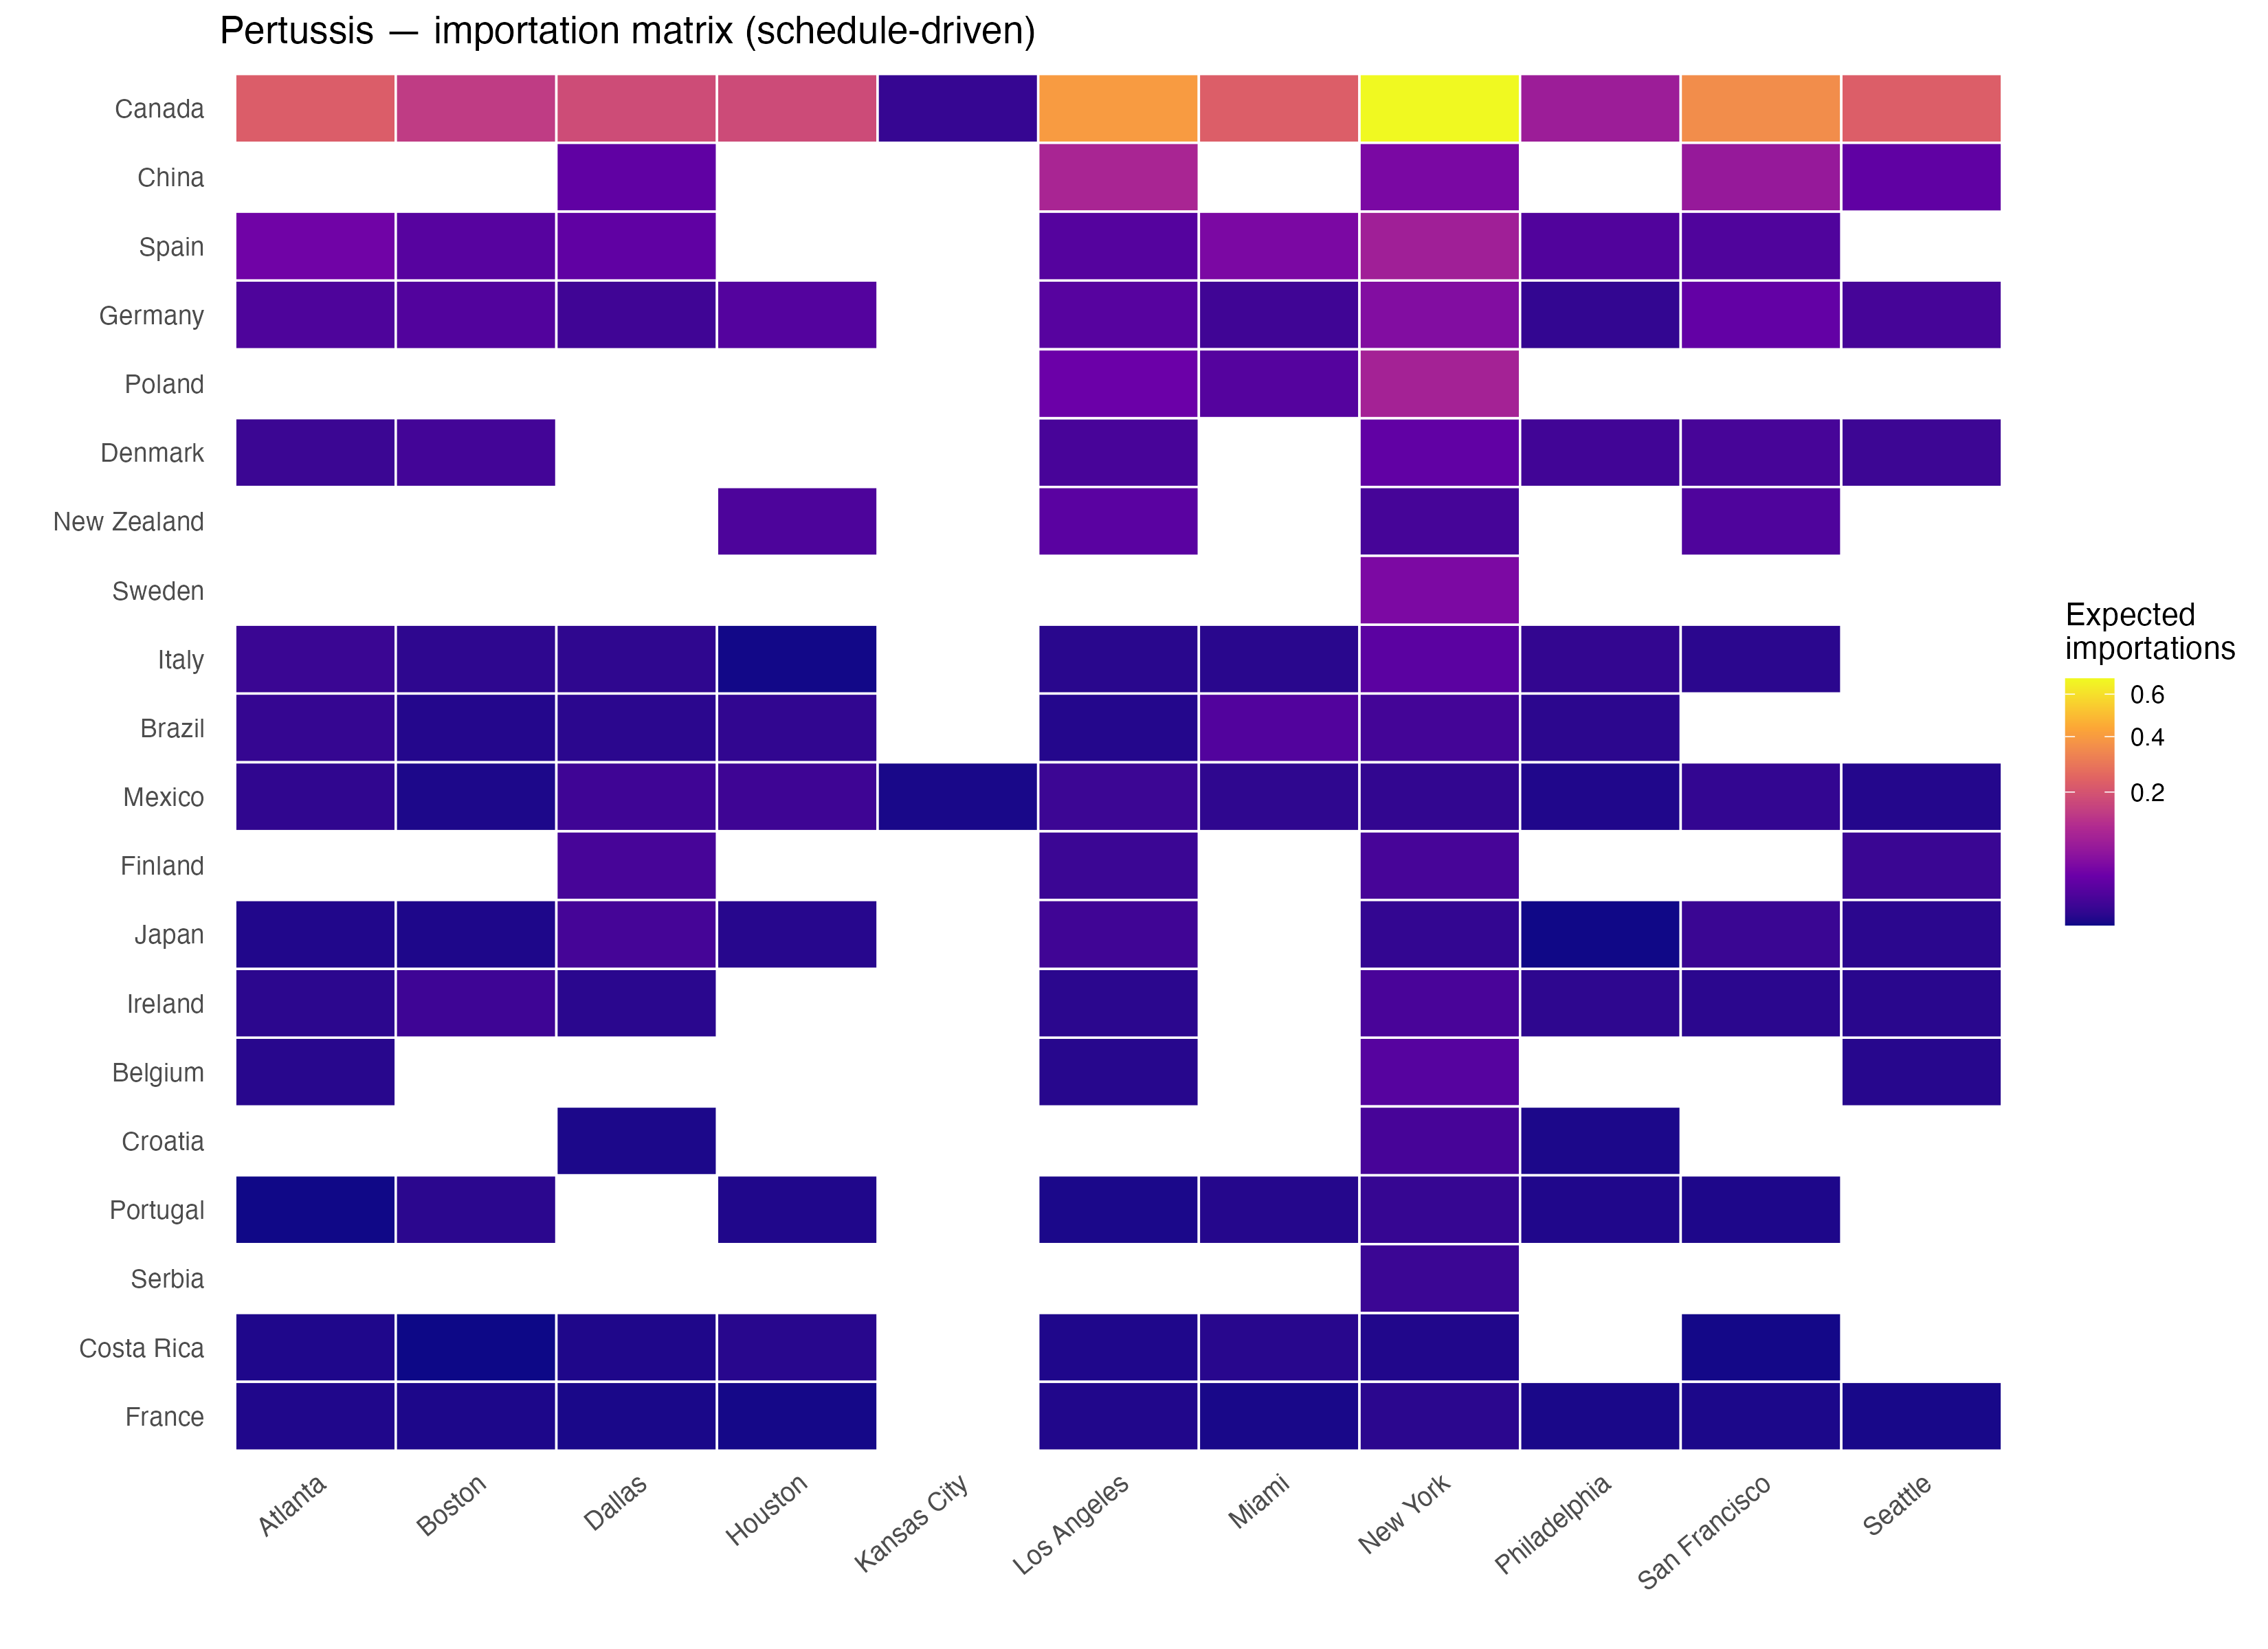
\includegraphics[width=\textwidth]{../Figures/heatmap_pertussis.png}
  \caption{Pertussis importation matrix. The broad geographic spread
    reflects pertussis's global endemicity and high
    travel-while-infectious probability ($p = 0.70$).}
  \label{fig:heatmap_pertussis}
\end{figure}

\begin{figure}[h!]
  \centering
  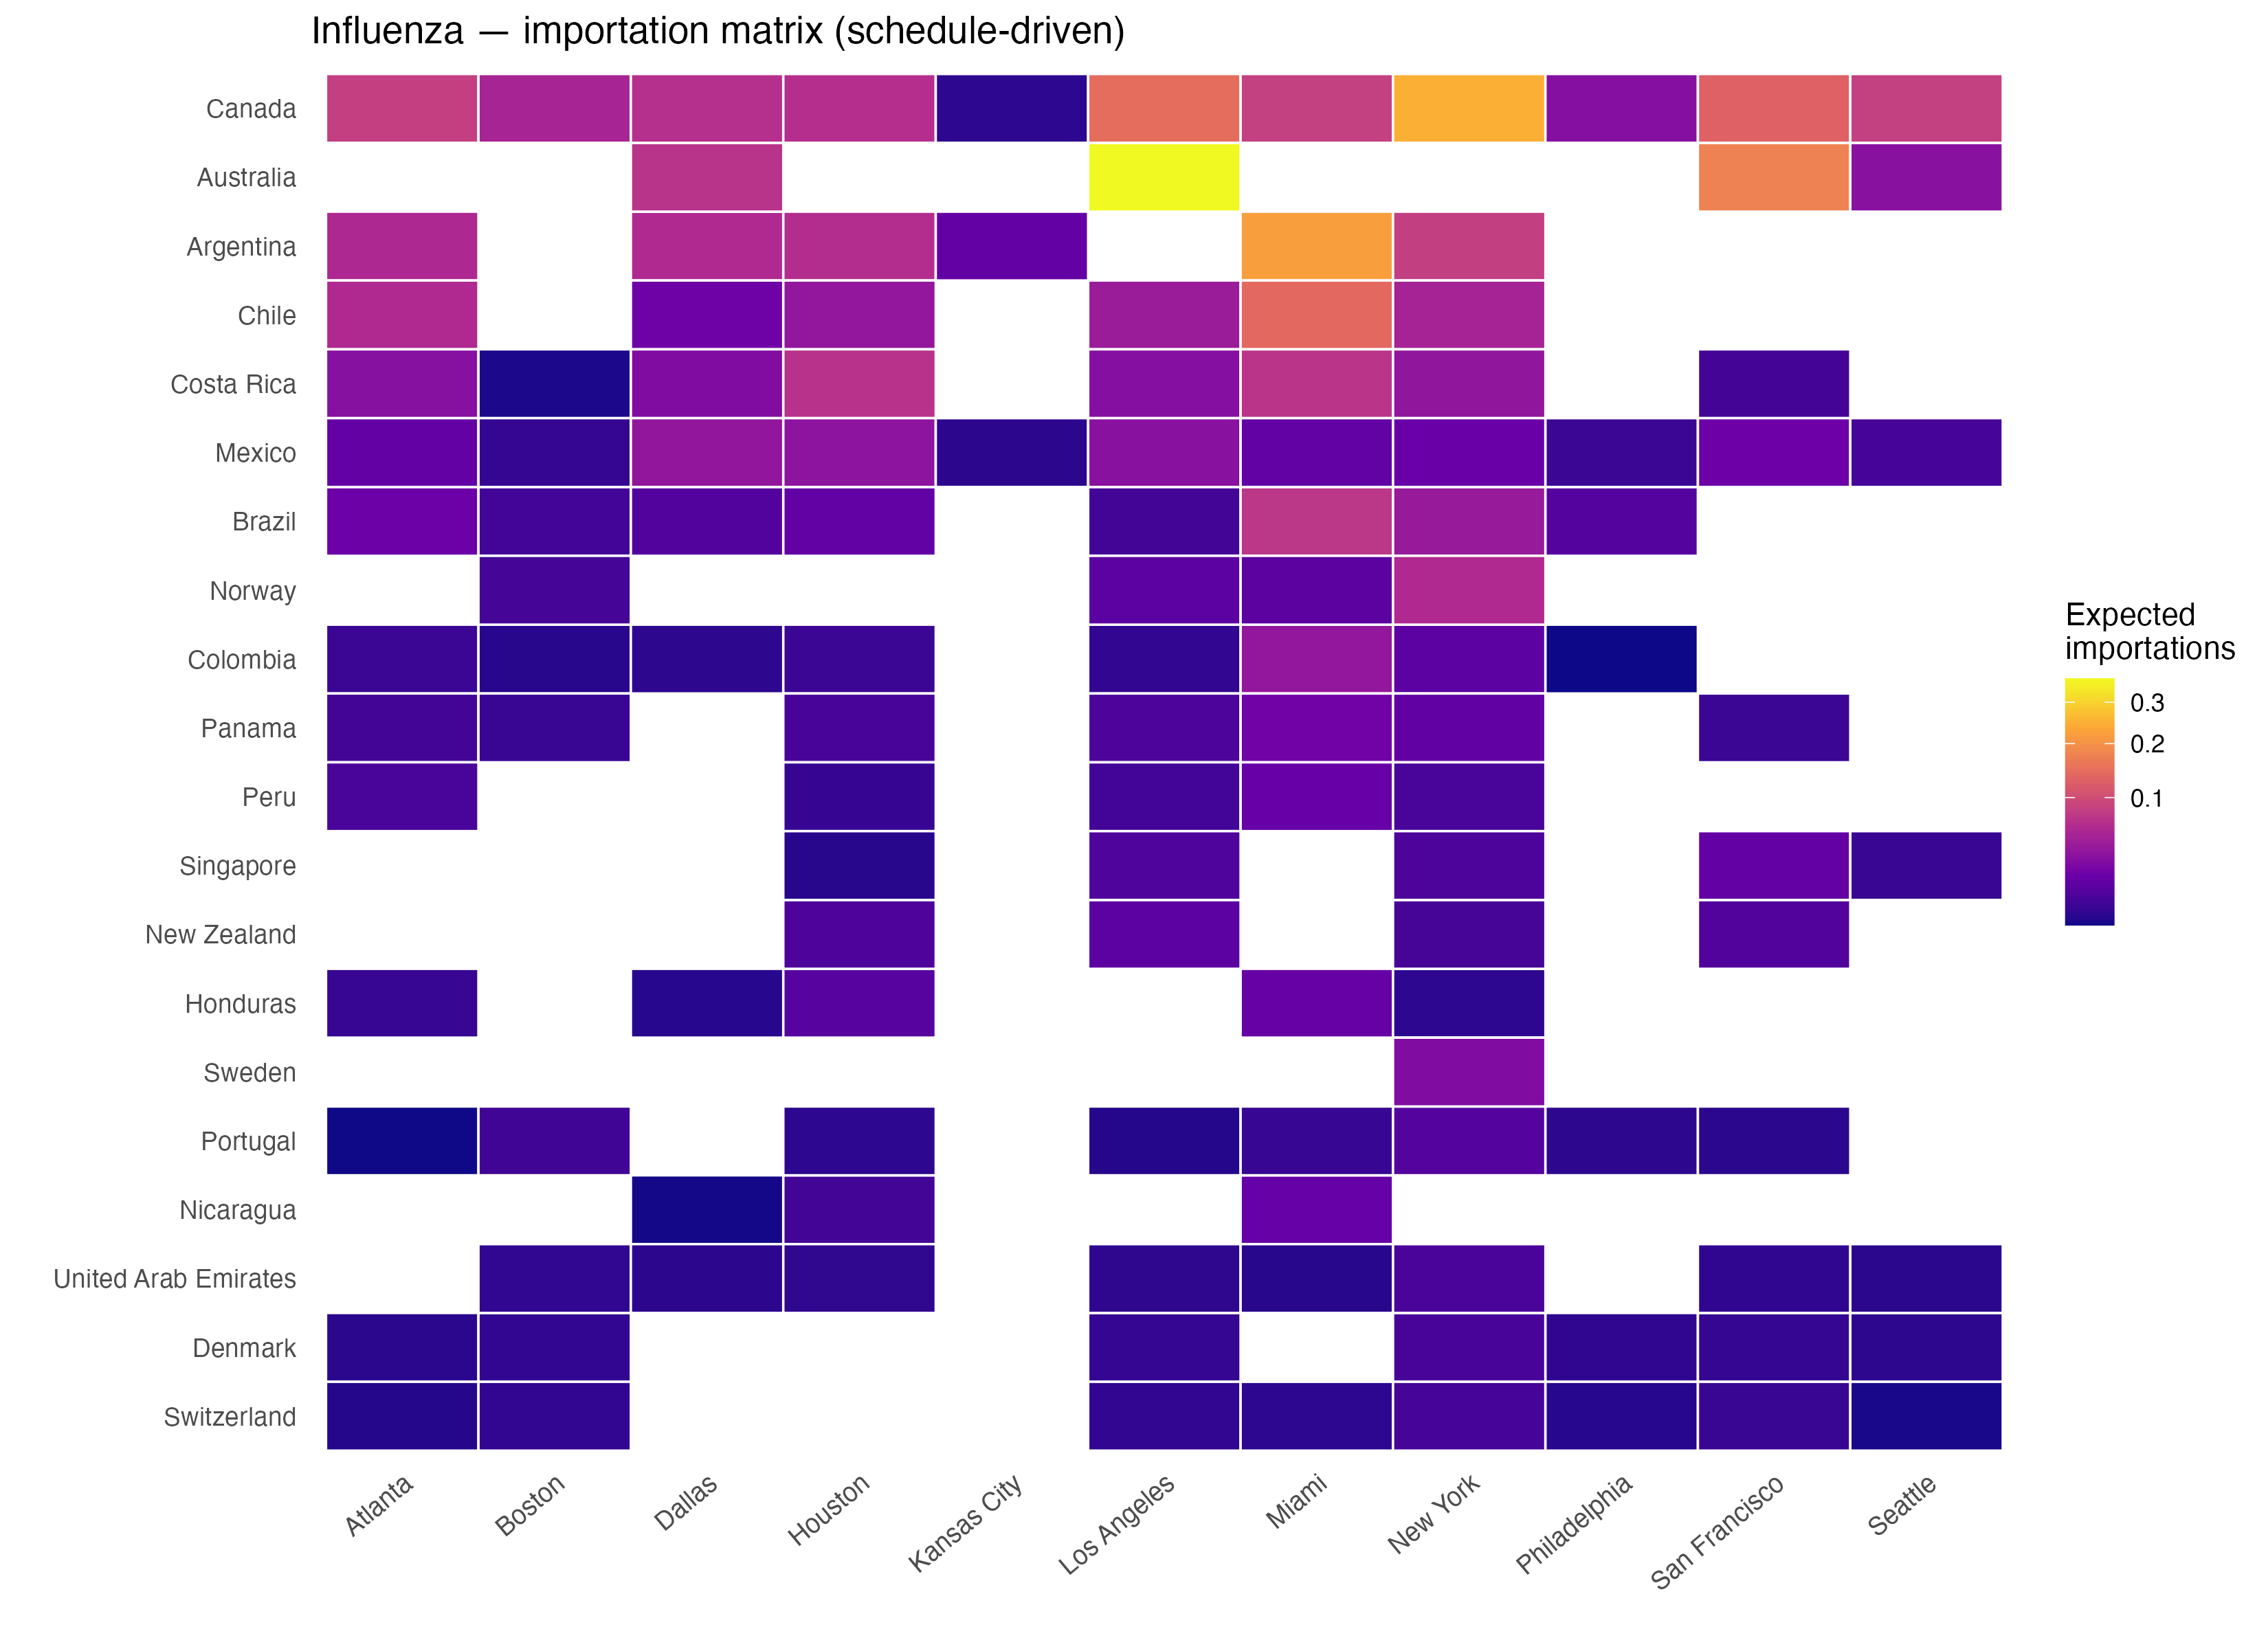
\includegraphics[width=\textwidth]{../Figures/heatmap_influenza.png}
  \caption{Influenza importation matrix: expected importations
    $\lambda_{c,v}$ by source country (rows, ordered by total burden)
    and destination city (columns) under the schedule-driven model.
    Plasma colour scale: bright yellow/orange = high; dark purple/blue = low.
    Risk is highest for Southern Hemisphere nations (Brazil, Argentina,
    Colombia) whose June peak transmission coincides with the tournament
    window. Background travel from high-volume non-qualified nations
    (e.g., Canada, Mexico, United Kingdom) contributes a broad diffuse
    signal across all cities.}
  \label{fig:heatmap_influenza}
\end{figure}

% ============================================================
\section*{Appendix C: Data Limitations and Improvement Opportunities}
% ============================================================

\subsection*{The role of non-public data in improving importation risk estimates}

The framework presented here relies entirely on publicly available
data sources --- a deliberate choice that ensures reproducibility and
allows the model to be updated by any public health team with internet
access. However, several categories of proprietary and restricted-access
data exist that would substantially improve the precision, timeliness,
and scope of the estimates, and their absence represents the primary
structural limitation of the current analysis.

The most valuable single dataset for this purpose would be
\textbf{airline booking and ticketing data}. Companies such as OAG
(Official Aviation Guide), Amadeus Travel Intelligence, and IATA's
PaxIS programme maintain origin-to-destination itinerary-level passenger
records that cover not only the nonstop international segment (as T-100
does) but the full trip, including domestic connecting legs to non-gateway
cities such as Kansas City and Seattle. These records are updated in
near-real time and can be filtered to the specific June--July 2026 travel
window rather than relying on historical routing fractions as a proxy for
future behavior. Similarly, \textbf{FIFA ticket sales records by country
of purchase}, while not publicly released, would replace the entire
WC-fan travel decomposition framework with a direct, event-specific
measure: rather than inferring WC fans from NTTO growth factors,
one could count the actual tickets sold to fans from each country and
allocate them to venue cities by the printed match schedule.

Beyond travel data, the precision of disease burden estimates is
constrained by the reliance on \textbf{WHO surveillance data}, which is
subject to reporting lags, inconsistent national case definitions, and
known under-ascertainment. National or regional health ministry
\textbf{line-list or case-count data} shared through WHO regional offices,
the Pan American Health Organization (PAHO), or the European Centre for
Disease Prevention and Control (ECDC) often contain more current and
complete figures than what appears in the publicly indexed datasets used
here --- particularly for dengue, where the 2025 season is not yet fully
incorporated. For measles and pertussis, \textbf{age-stratified incidence
and national vaccination coverage data} at the subnational level (available
from national immunization programmes but not systematically published)
would substantially improve the per-traveler infection probability
$I_{c,d}$ by accounting for the fact that international travelers skew
toward working-age adults, who may have markedly different immunity and
infection rates than the general population.

Finally, the current model estimates importation risk but stops short
of estimating local transmission risk after importation. Extending the
framework in that direction would require \textbf{local
\textit{Aedes aegypti} vector surveillance data} from state and
county health departments (partially available through CDC ArboNET but
not consistently in machine-readable form), \textbf{hospital and
public health capacity data} by city and county (available through
the American Hospital Association survey but behind a licensing
agreement), and \textbf{aggregated mobility data} from mobile device
providers (Meta, Google) to calibrate the spatial spread of fans
within and between cities. None of these datasets are currently
accessible through open public APIs at the geographic resolution
needed for this analysis. Establishing data-sharing agreements with
the relevant agencies and commercial providers before the tournament
begins --- ideally through the CDC's International Importation
Response Branch or the Council of State and Territorial Epidemiologists
(CSTE) --- would allow these estimates to be refined and operationalized
in real time during June--July 2026.

% ============================================================
\newpage
\section*{Appendix D: Qualified Nations — 2026 FIFA World Cup}
% ============================================================

\begin{longtable}{llc}
\toprule
\textbf{Country} & \textbf{Confederation} & \textbf{Host nation} \\
\midrule
\endfirsthead
\toprule
\textbf{Country} & \textbf{Confederation} & \textbf{Host nation} \\
\midrule
\endhead
\midrule
\multicolumn{3}{r}{\textit{Continued on next page}} \\
\endfoot
\bottomrule
\endlastfoot
% --- AFC (9) ---
Japan          & AFC & No \\
Iran           & AFC & No \\
South Korea    & AFC & No \\
Australia      & AFC & No \\
Qatar          & AFC & No \\
Saudi Arabia   & AFC & No \\
Uzbekistan     & AFC & No \\
Jordan         & AFC & No \\
Iraq           & AFC & No \\
% --- CAF (10) ---
Morocco        & CAF & No \\
Tunisia        & CAF & No \\
Egypt          & CAF & No \\
Algeria        & CAF & No \\
Ghana          & CAF & No \\
Cape Verde     & CAF & No \\
Senegal        & CAF & No \\
South Africa   & CAF & No \\
Ivory Coast    & CAF & No \\
DR Congo       & CAF & No \\
% --- CONCACAF (6) ---
Canada         & CONCACAF & Yes \\
Mexico         & CONCACAF & Yes \\
United States  & CONCACAF & Yes \\
Panama         & CONCACAF & No \\
Cura\c{c}ao   & CONCACAF & No \\
Haiti          & CONCACAF & No \\
% --- CONMEBOL (6) ---
Argentina      & CONMEBOL & No \\
Brazil         & CONMEBOL & No \\
Ecuador        & CONMEBOL & No \\
Paraguay       & CONMEBOL & No \\
Uruguay        & CONMEBOL & No \\
Colombia       & CONMEBOL & No \\
% --- UEFA (16) ---
England        & UEFA & No \\
France         & UEFA & No \\
Croatia        & UEFA & No \\
Portugal       & UEFA & No \\
Norway         & UEFA & No \\
Germany        & UEFA & No \\
Netherlands    & UEFA & No \\
Switzerland    & UEFA & No \\
Scotland       & UEFA & No \\
Spain          & UEFA & No \\
Austria        & UEFA & No \\
Belgium        & UEFA & No \\
Bosnia and Herzegovina & UEFA & No \\
Sweden         & UEFA & No \\
Turkey         & UEFA & No \\
Czech Republic & UEFA & No \\
% --- OFC (1) ---
New Zealand    & OFC & No \\
\end{longtable}

\noindent\small
\textit{Note}: Confederation abbreviations --- AFC: Asian Football
Confederation; CAF: Confederation of African Football; CONCACAF:
Confederation of North, Central America and Caribbean Association
Football; CONMEBOL: South American Football Confederation; UEFA:
Union of European Football Associations; OFC: Oceania Football
Confederation. Source: \url{https://en.wikipedia.org/wiki/2026_FIFA_World_Cup_qualification}
(accessed April 2026).

\end{document}
